Selections are applied to selects events compatible with containing a $bb\tau_{had}\tau_{had}$ final state. This selection forms the signal region containing the set of events that are used for the fit of the MVA discriminant distributions as described in Section~\ref{sec:fit}. 

All events passing the trigger selection must then meet the following requirements (using the object definitions described in Section~\ref{sec:reco}):

\begin{itemize}
\item At least two jets;
\item Exactly two $\tau$-leptons passing the `loose' identification criteria;
\item No electrons or muons in the event;
\item Exactly two $b$-tagged jets (using DL1r 77\% working point);
\item Opposite-sign charge between the two $\tau$-leptons;
\item The invariant mass of the di-$\tau$ system (calculated using the Missing Mass Calculator (MMC) \cite{Elagin:2010aw}),
  $\mMMC_{\tau\tau}$, must be > 60 $\GeV$;
\item At least one \bjet with \pT > \SI{45}{\GeV}. %\todo{Chris: maybe we
  % shoulddrop this selection?}
\item The subleading \tauhad candidate is required to have $\pT > \SI{25}{\GeV}$
  (this is due to a $\SI{23}{\GeV}$ requirement in the HIGG4D3 derivation skim)
\end{itemize}

For STT events one of the two $\tau_{had}$ has to be matched to the object that fired the trigger, for DTT events both $\tau_{had}$ have to be matched to the objects that fired the trigger.

The \pt thresholds applied on the jets and the $\tau$-leptons depend on the trigger applied. The summary of the \pT thresholds applied is as follows:
\begin{itemize}
\item STT events: \tauhadvis are required to pass a trigger-dependent
  \pT threshold as described in
  \cref{sec:hadhad_trigger_selection}. Only if the event was not
  selected by the STT relevant for the particular run (even if the
  event was selected by a di-\tauhad trigger), it is checked whether
  the event passes the DTT selection (i.e.\ STT events are prioritized
  over DTT events).

\item DTT events in 2015-2016: The leading jet is required to have \pT >
  \SI{80}{\GeV} due to the additional jet requirement (J25) at L1 in 2016. This
  ensures that the L1 trigger is close to its efficiency plateau, minimizing the
  impact of a mismatch in trigger efficiency in data / MC.

\item DTT events in 2017-2018: Are categorised into two categories depending on
  the triggers to be checked: %\todo{Chris: need to check treatment of non-L1Topo trigger at the beginning of 2017}
  \begin{itemize}
  \item If leading and subleading jet $\pT > \SI{45}{\GeV}$: Event is considered a
    4J12 event. This cut ensures that the additional jet requirement at L1 (J12)
    is fulfilled.
  \item Else if leading jet $\pT > \SI{80}{\GeV}$ and $\dRtautau \leq 2.5$:
    Event is considered a L1Topo event. The jet \pT and \dRtautau cut ensure
    that the additional J25 and \dRtautau requirement at L1 are fulfilled.
  \end{itemize}
\end{itemize}

Figure~\ref{fig:HadHadPreselectionPtDistributions} shows data/prediction comparison for \tauhad \pt and $\eta$ and $b$-jets \pt pre-fit after applying the $bb\tau_{had}\tau_{had}$ event selection (these distributions are not blinded as the definition of the signal region selection is very loose as to define a pre-selection region and MVAs are then used in this region to separate background and signal). The background estimation and the systematic uncertainties included in these plots are discussed in Section~\ref{sec:bkg} and Section~\ref{sec:systs} respectively. Figures~\ref{fig:HadHadPreselectionPtDistributions2015}-~\ref{fig:HadHadPreselectionPtDistributions2018} show the same distributions split by data-taking period.

Additional plots split by trigger and also in validation regions are given in Appendix~\ref{subsec:appendix_bkg_validation_hadhad}.

%\begin{figure}
%\centering
%\subfloat[]
%   {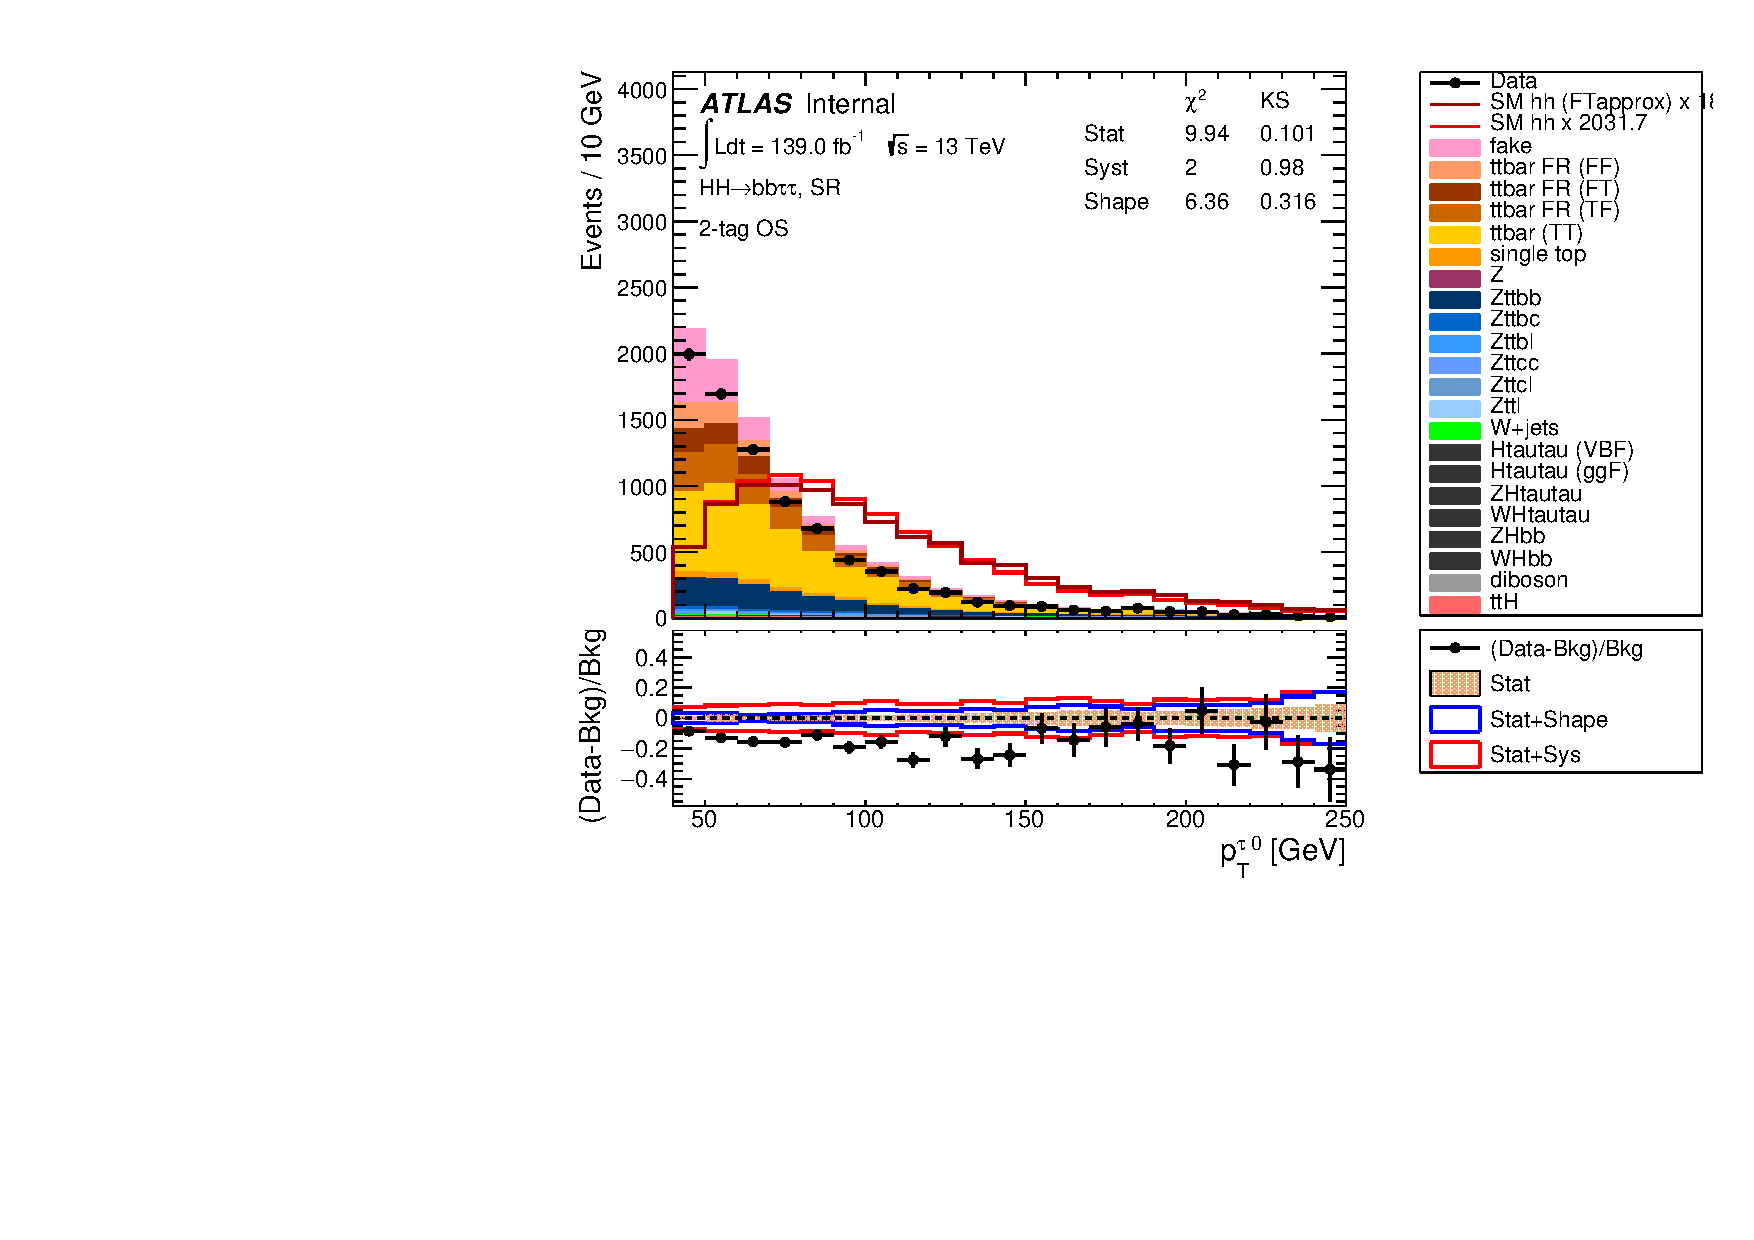
\includegraphics[width=.45\textwidth]{figures/selection/HadHad_HH/C_2tag2pjet_0ptv_LL_OS_Tau0Pt.pdf}}\quad
%\subfloat[]
%   {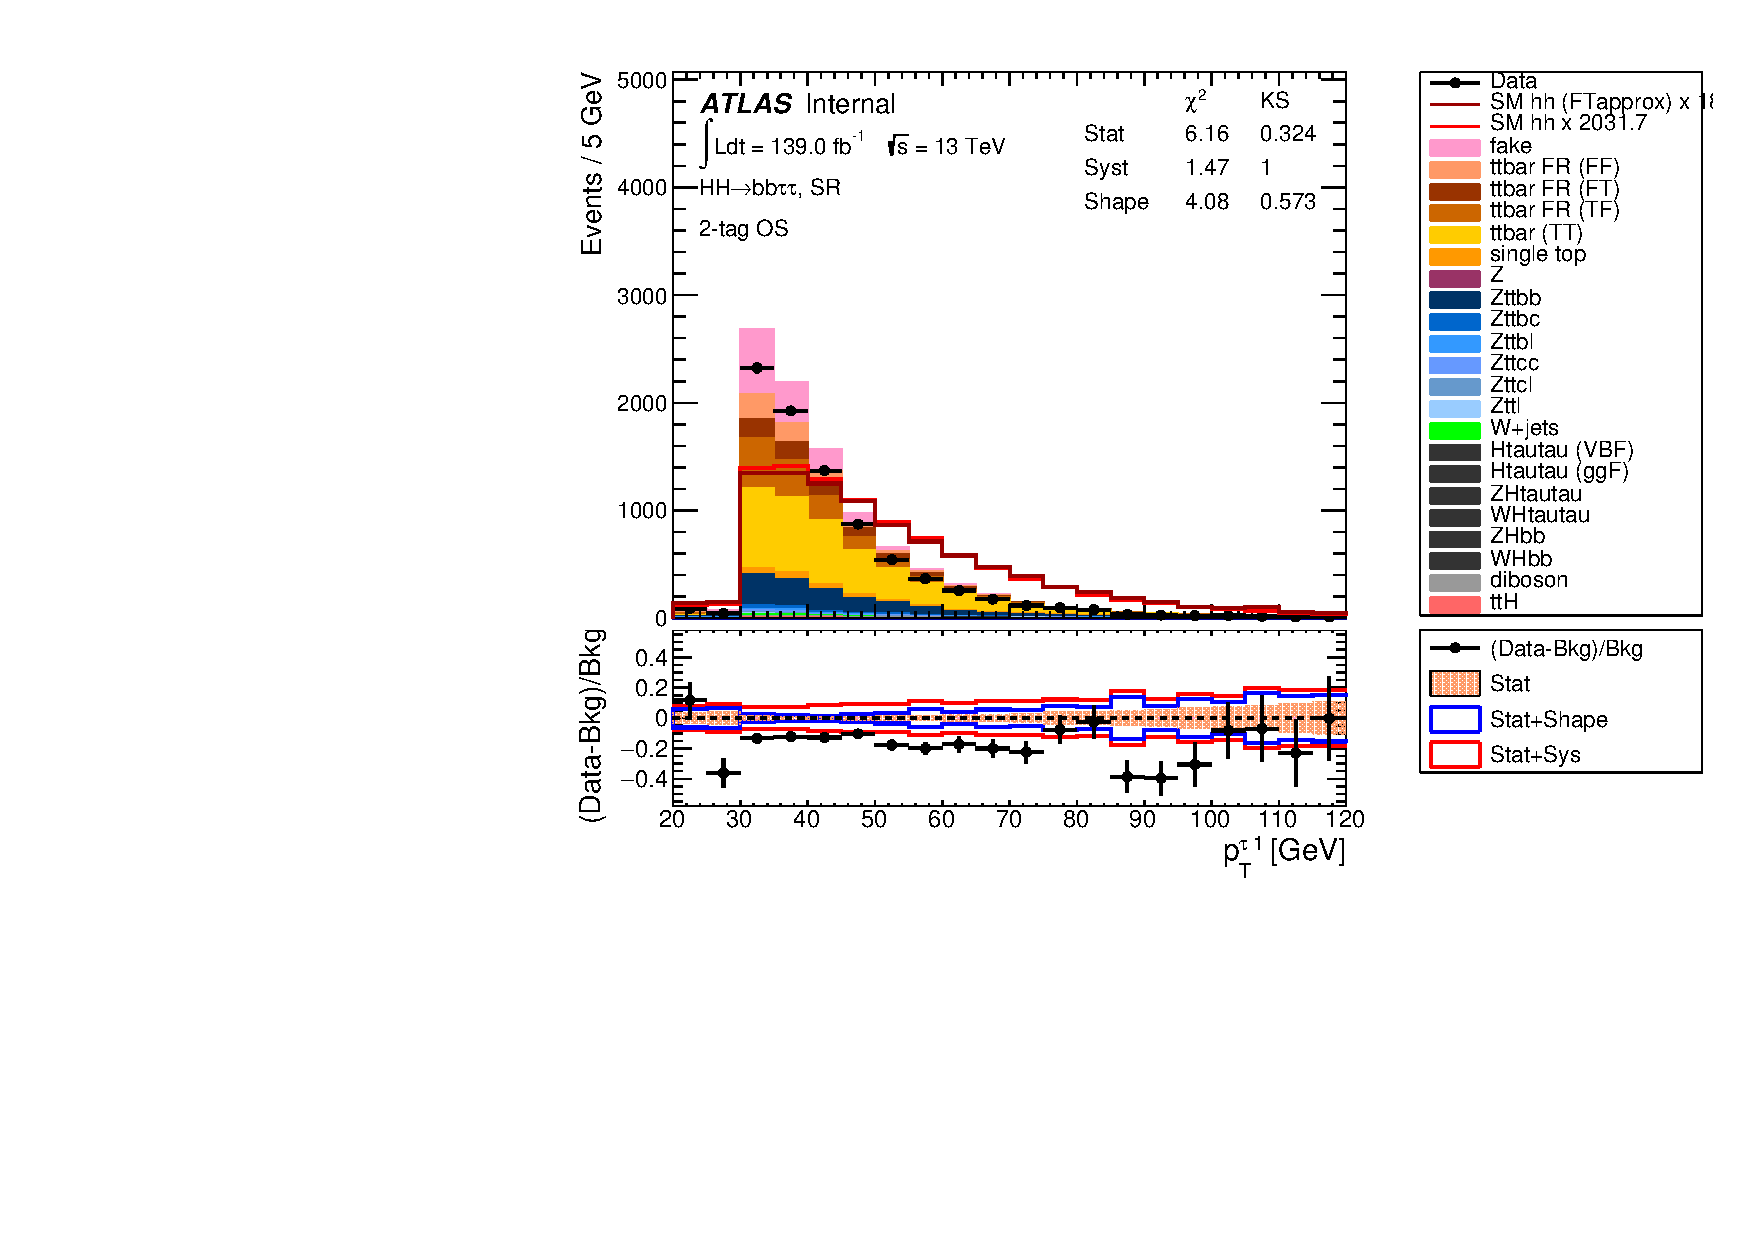
\includegraphics[width=.45\textwidth]{figures/selection/HadHad_HH/C_2tag2pjet_0ptv_LL_OS_Tau1Pt.pdf}} \quad
%\subfloat[]
%   {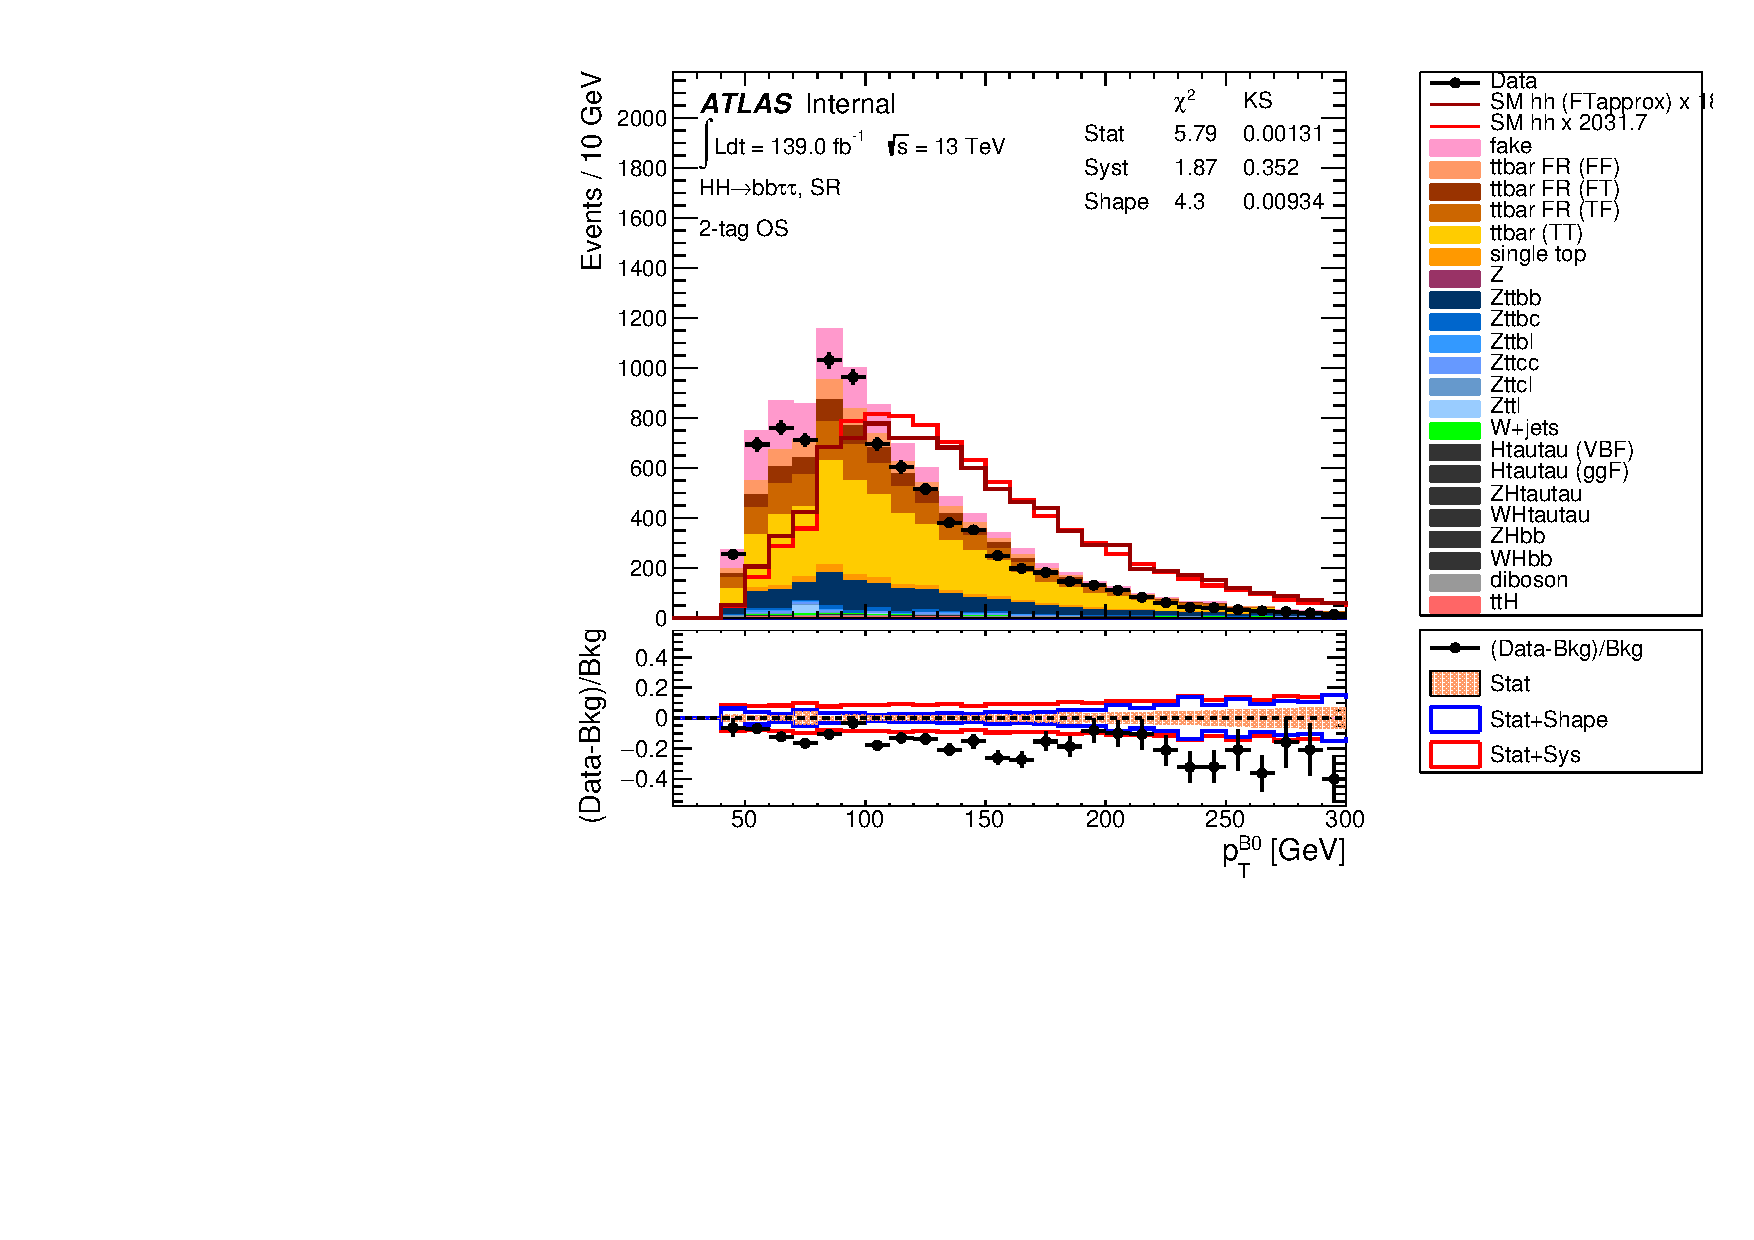
\includegraphics[width=.45\textwidth]{figures/selection/HadHad_HH/C_2tag2pjet_0ptv_LL_OS_pTB0.pdf}}\quad
%\subfloat[]
%   {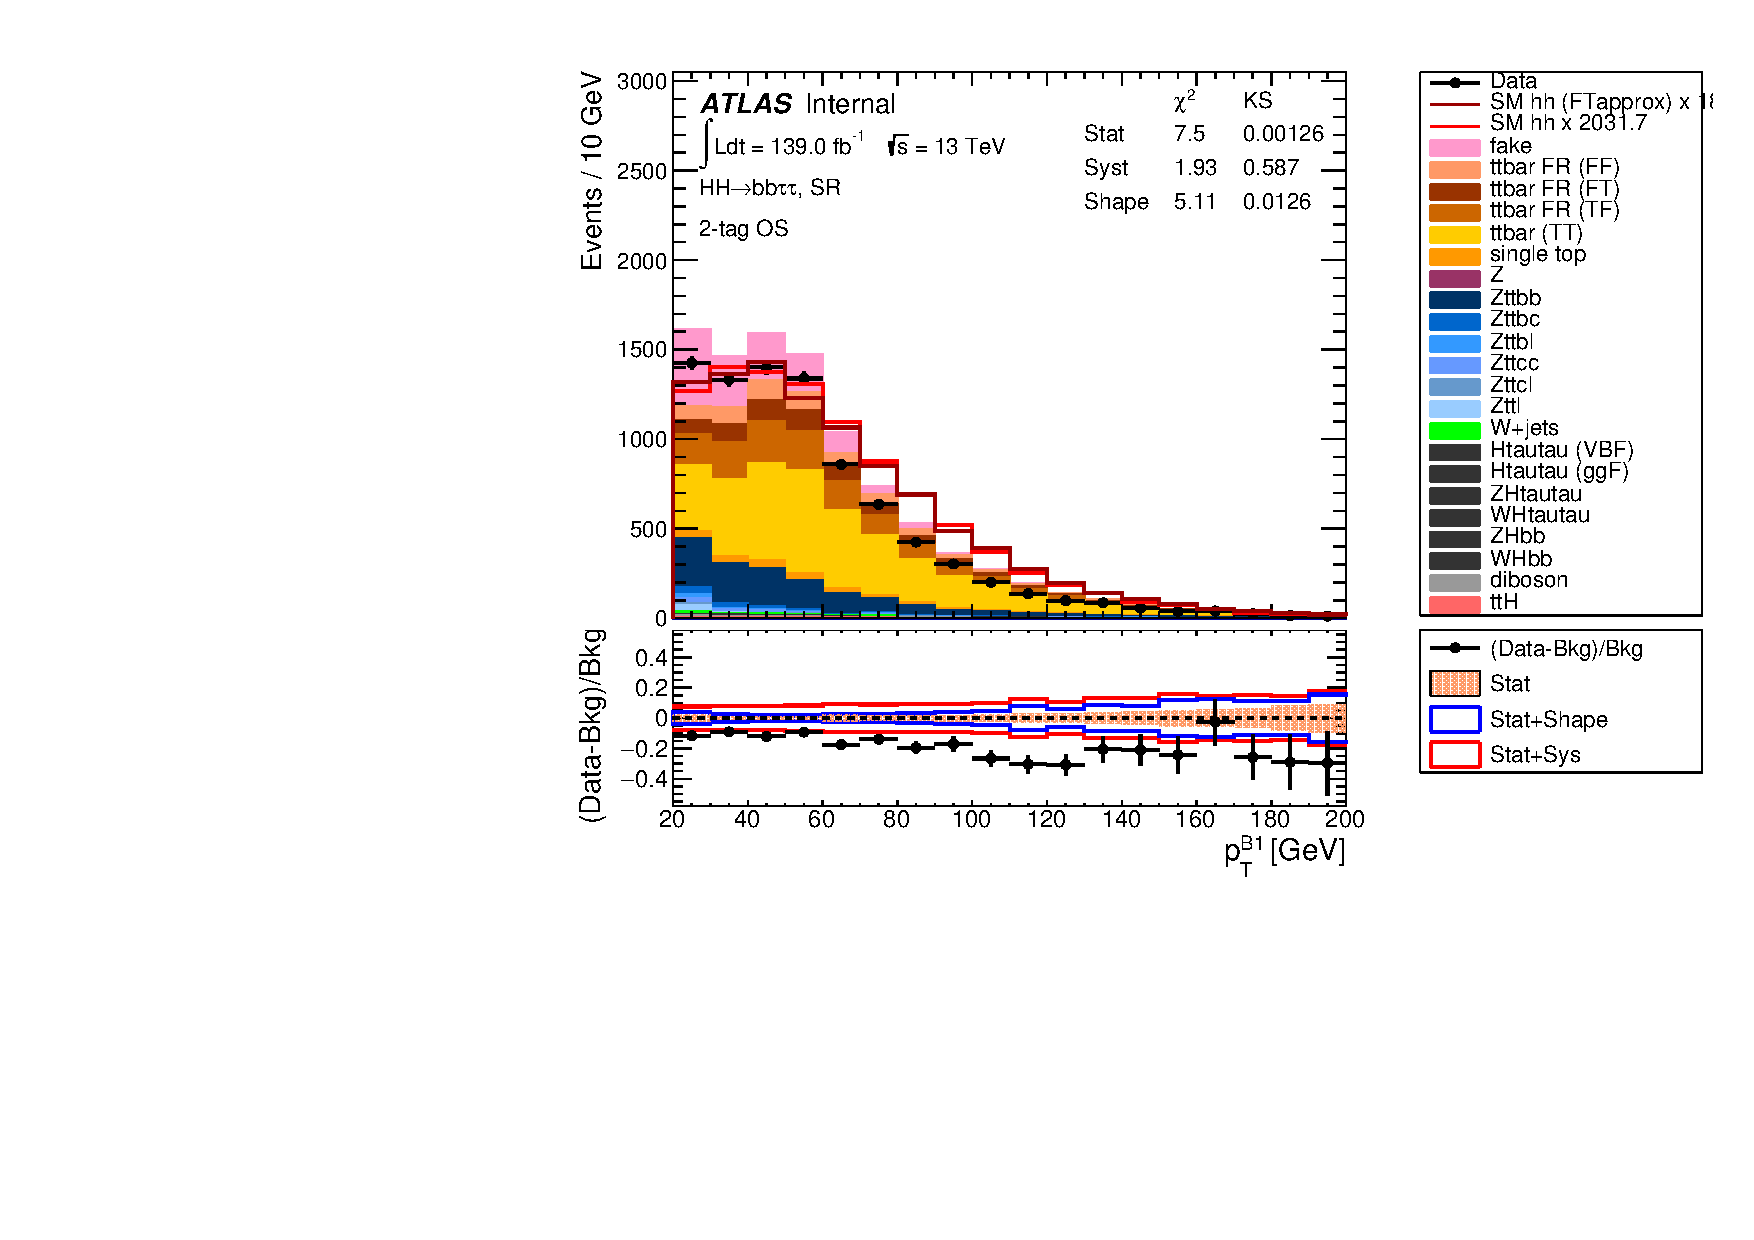
\includegraphics[width=.45\textwidth]{figures/selection/HadHad_HH/C_2tag2pjet_0ptv_LL_OS_pTB1.pdf}} \quad
%\caption{Leading and sub-leading $\tau_{had}$ and $b$-jet pre-fit \pt
%  distributions in the di-Higgs $bb\tau_{had}\tau_{had}$ signal region. The yields for Zttbb, Zttbc and Zttcc are scaled by 1.3. The uncertainty band includes CP uncertainties and $t\bar{t}$ and fake-$\tau_{had}$ backgrounds modelling uncertainties. (Inputs from 2020\_10\_16) (\textcolor{red}{To do: replace with plots from WSMaker including all uncertainties})}
%\label{fig:HadHadPreselectionPtDistributions}
%\end{figure}

\begin{figure}
\centering
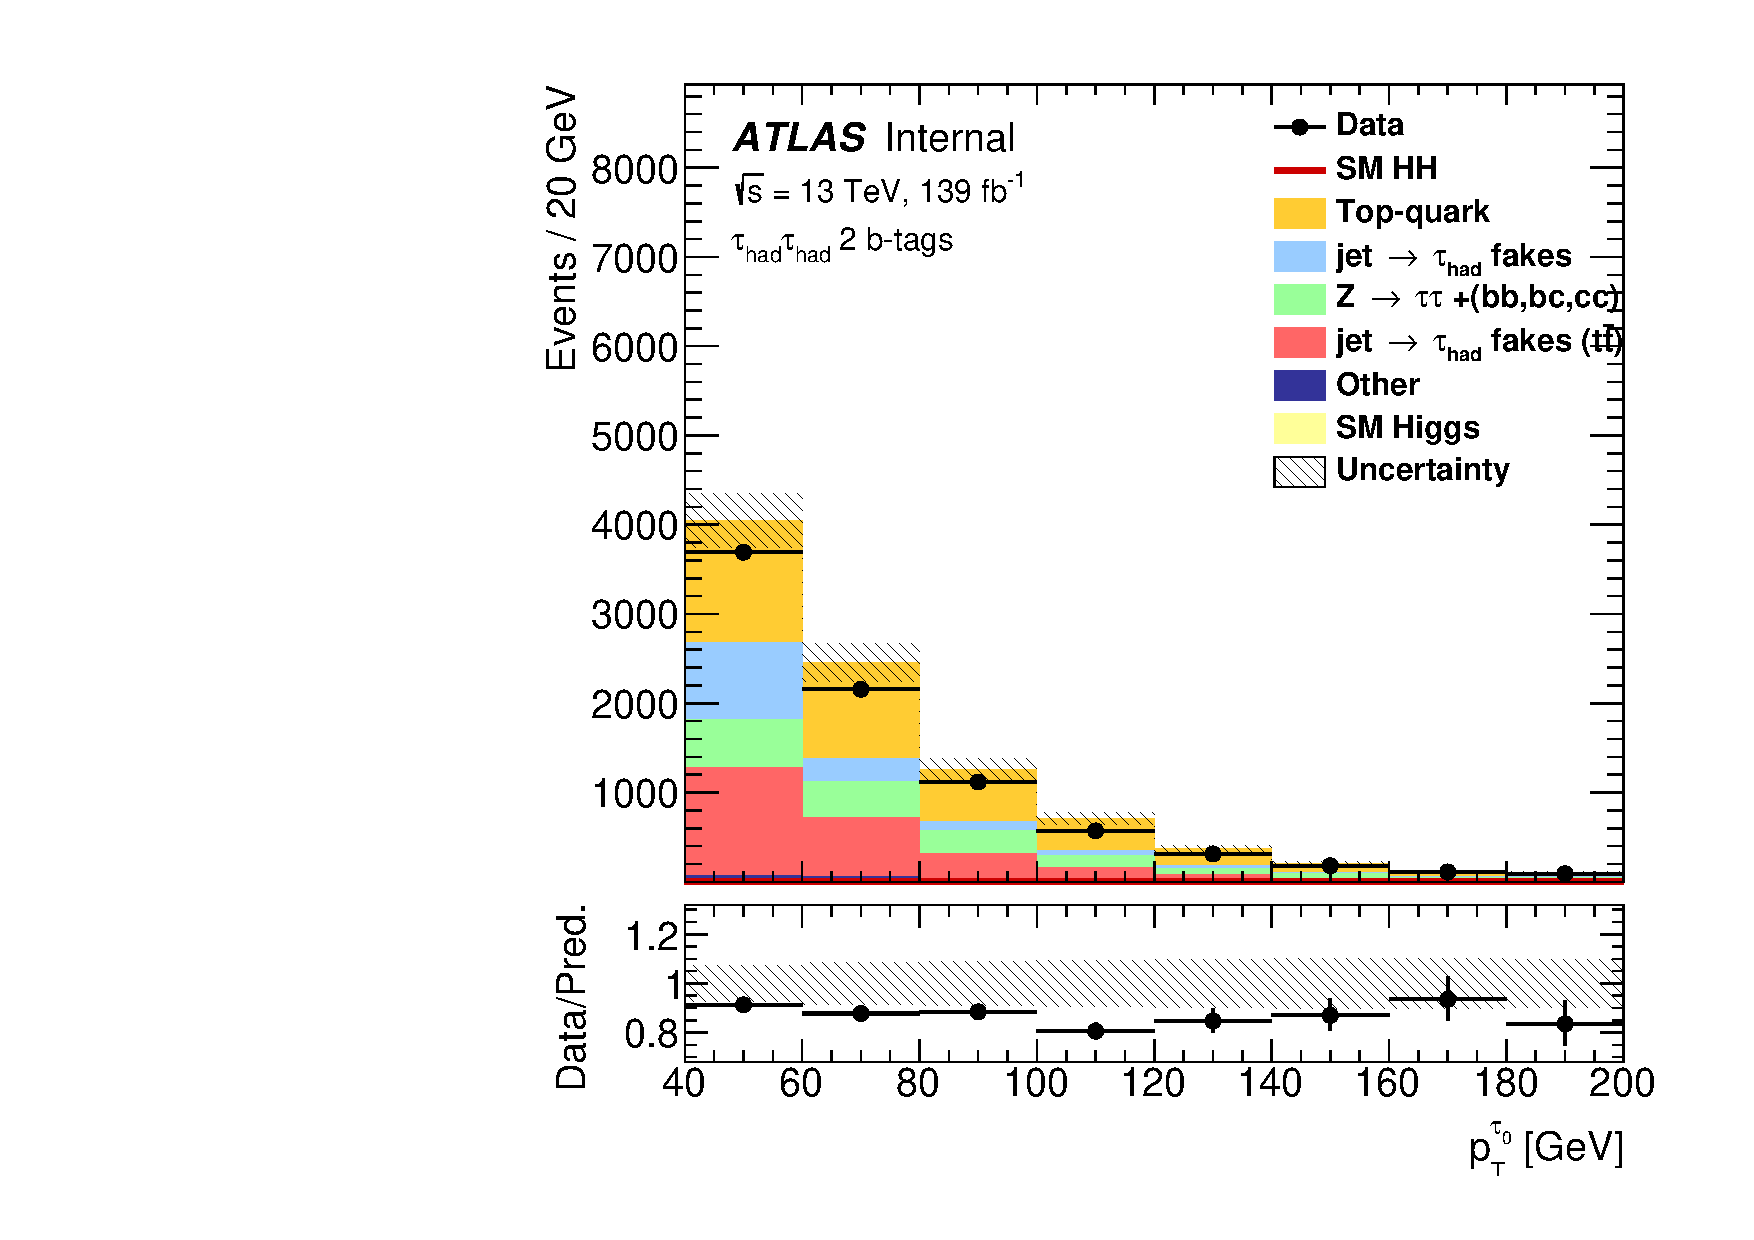
\includegraphics[width=.45\textwidth]{figures/selection/HadHad_HH/Region_BMin0_incJet1_distTau0Pt_J2_Y2015_DLLOS_T2_SpcTauHH_L0_Prefit.pdf}
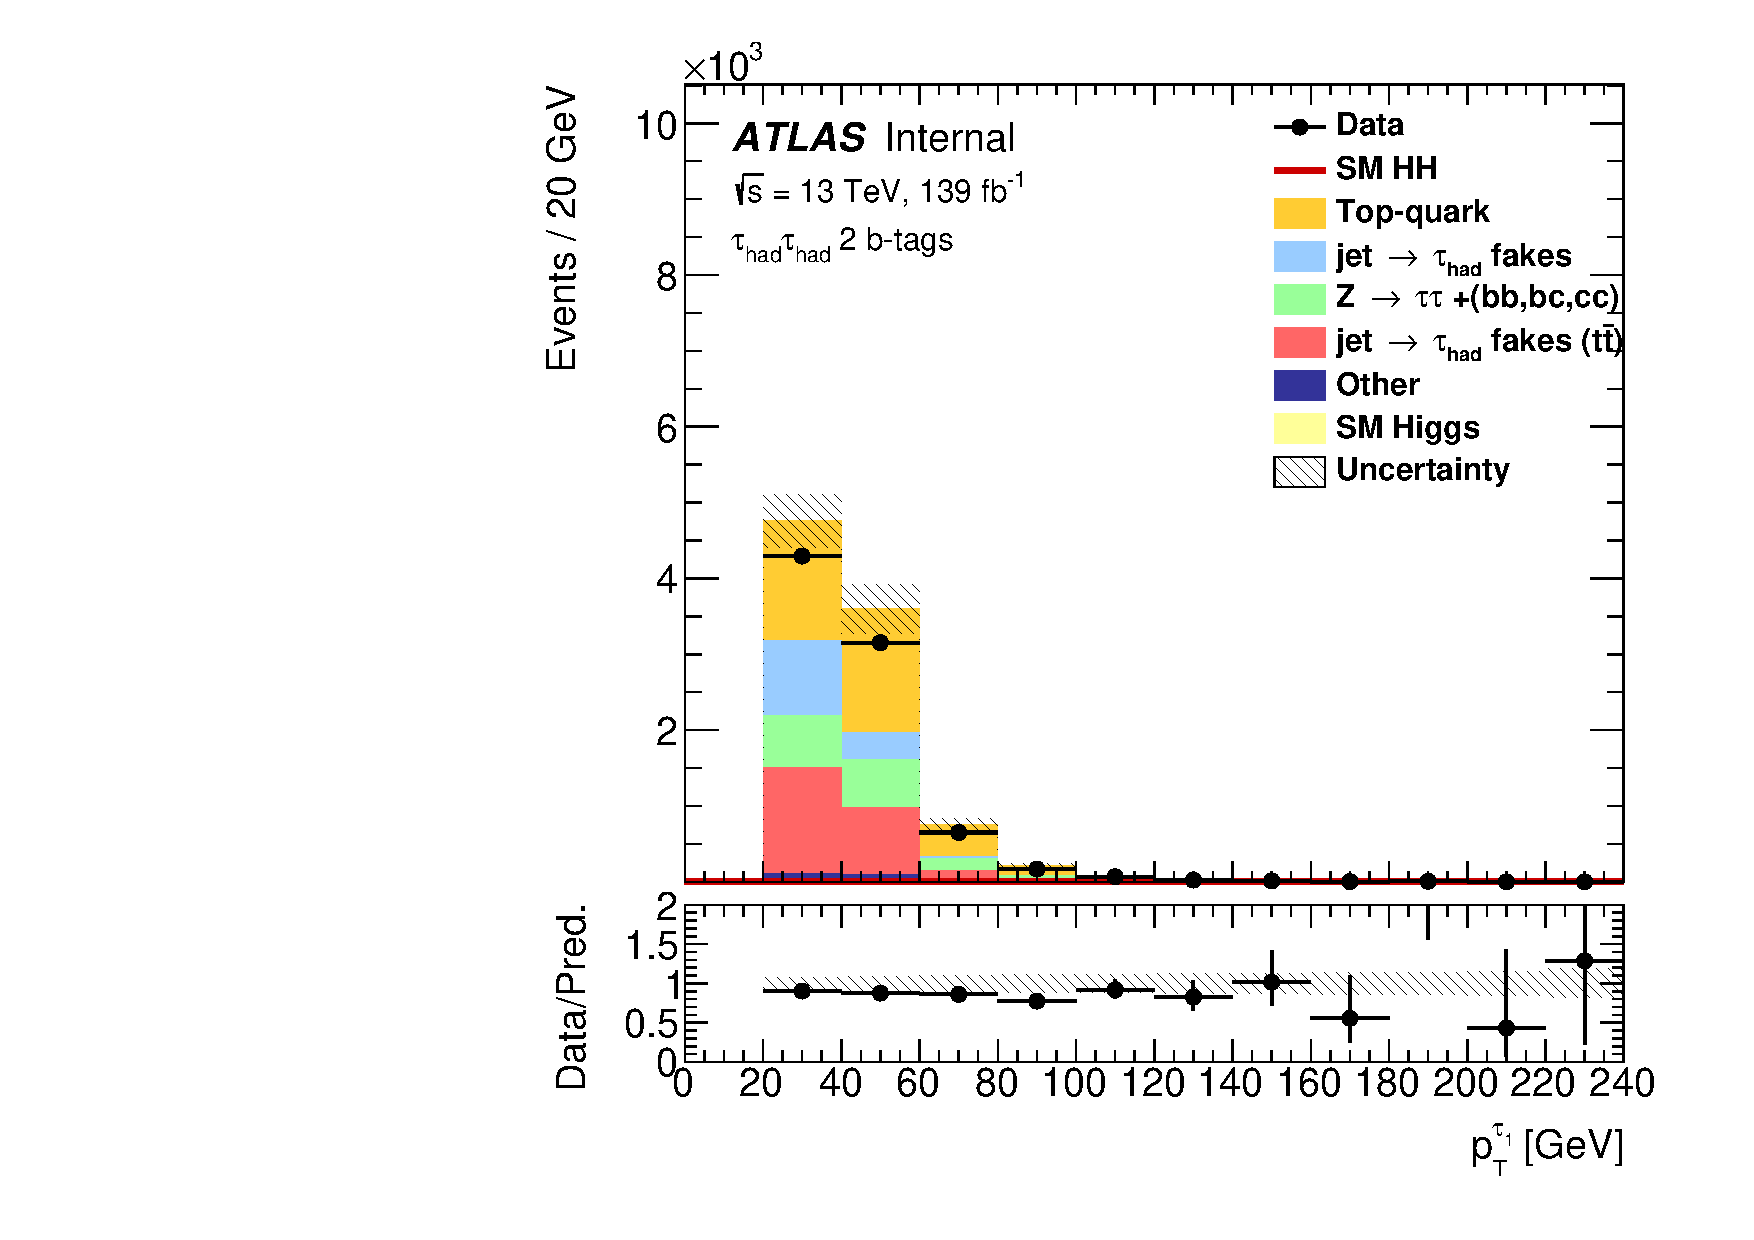
\includegraphics[width=.45\textwidth]{figures/selection/HadHad_HH/Region_BMin0_incJet1_distTau1Pt_J2_Y2015_DLLOS_T2_SpcTauHH_L0_Prefit.pdf}\\
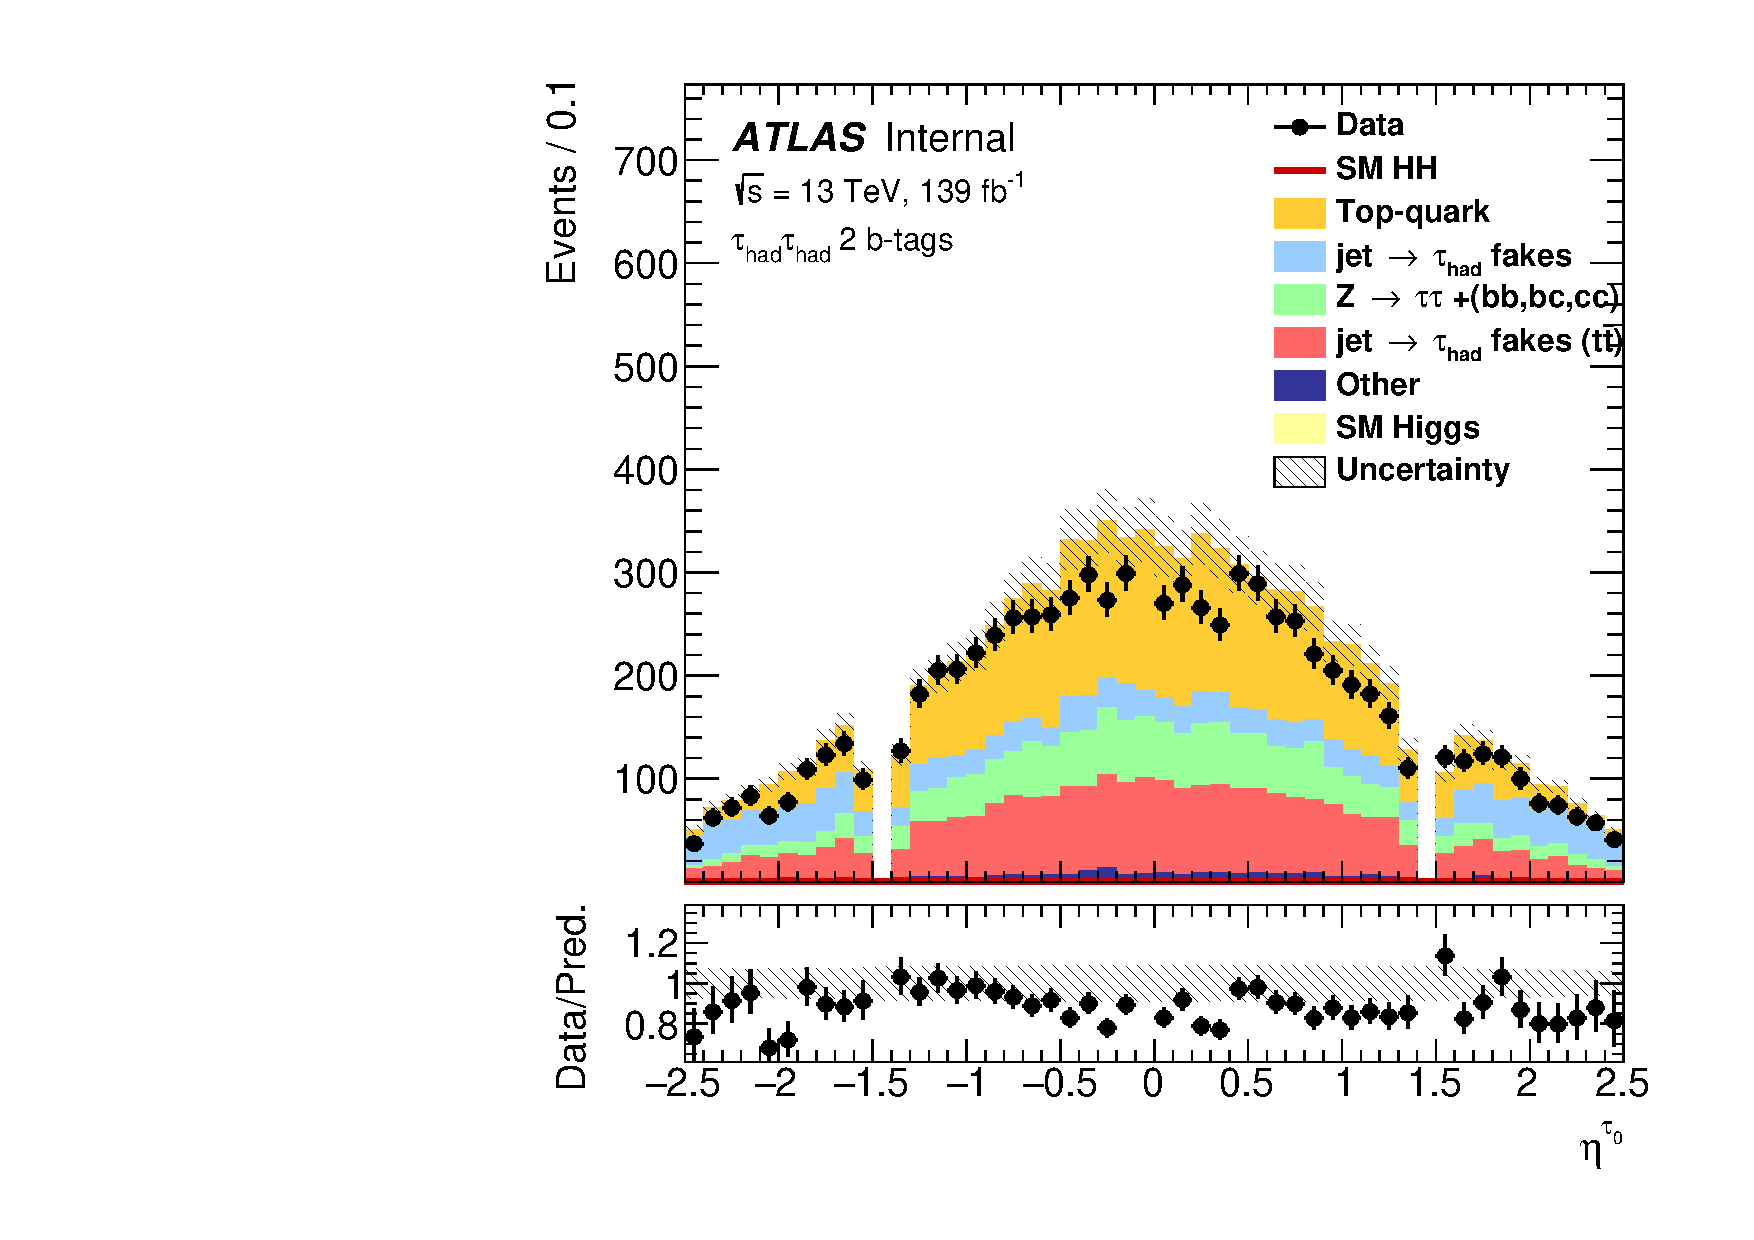
\includegraphics[width=.45\textwidth]{figures/selection/HadHad_HH/Region_BMin0_incJet1_distTau0Eta_J2_Y2015_DLLOS_T2_SpcTauHH_L0_Prefit.pdf}
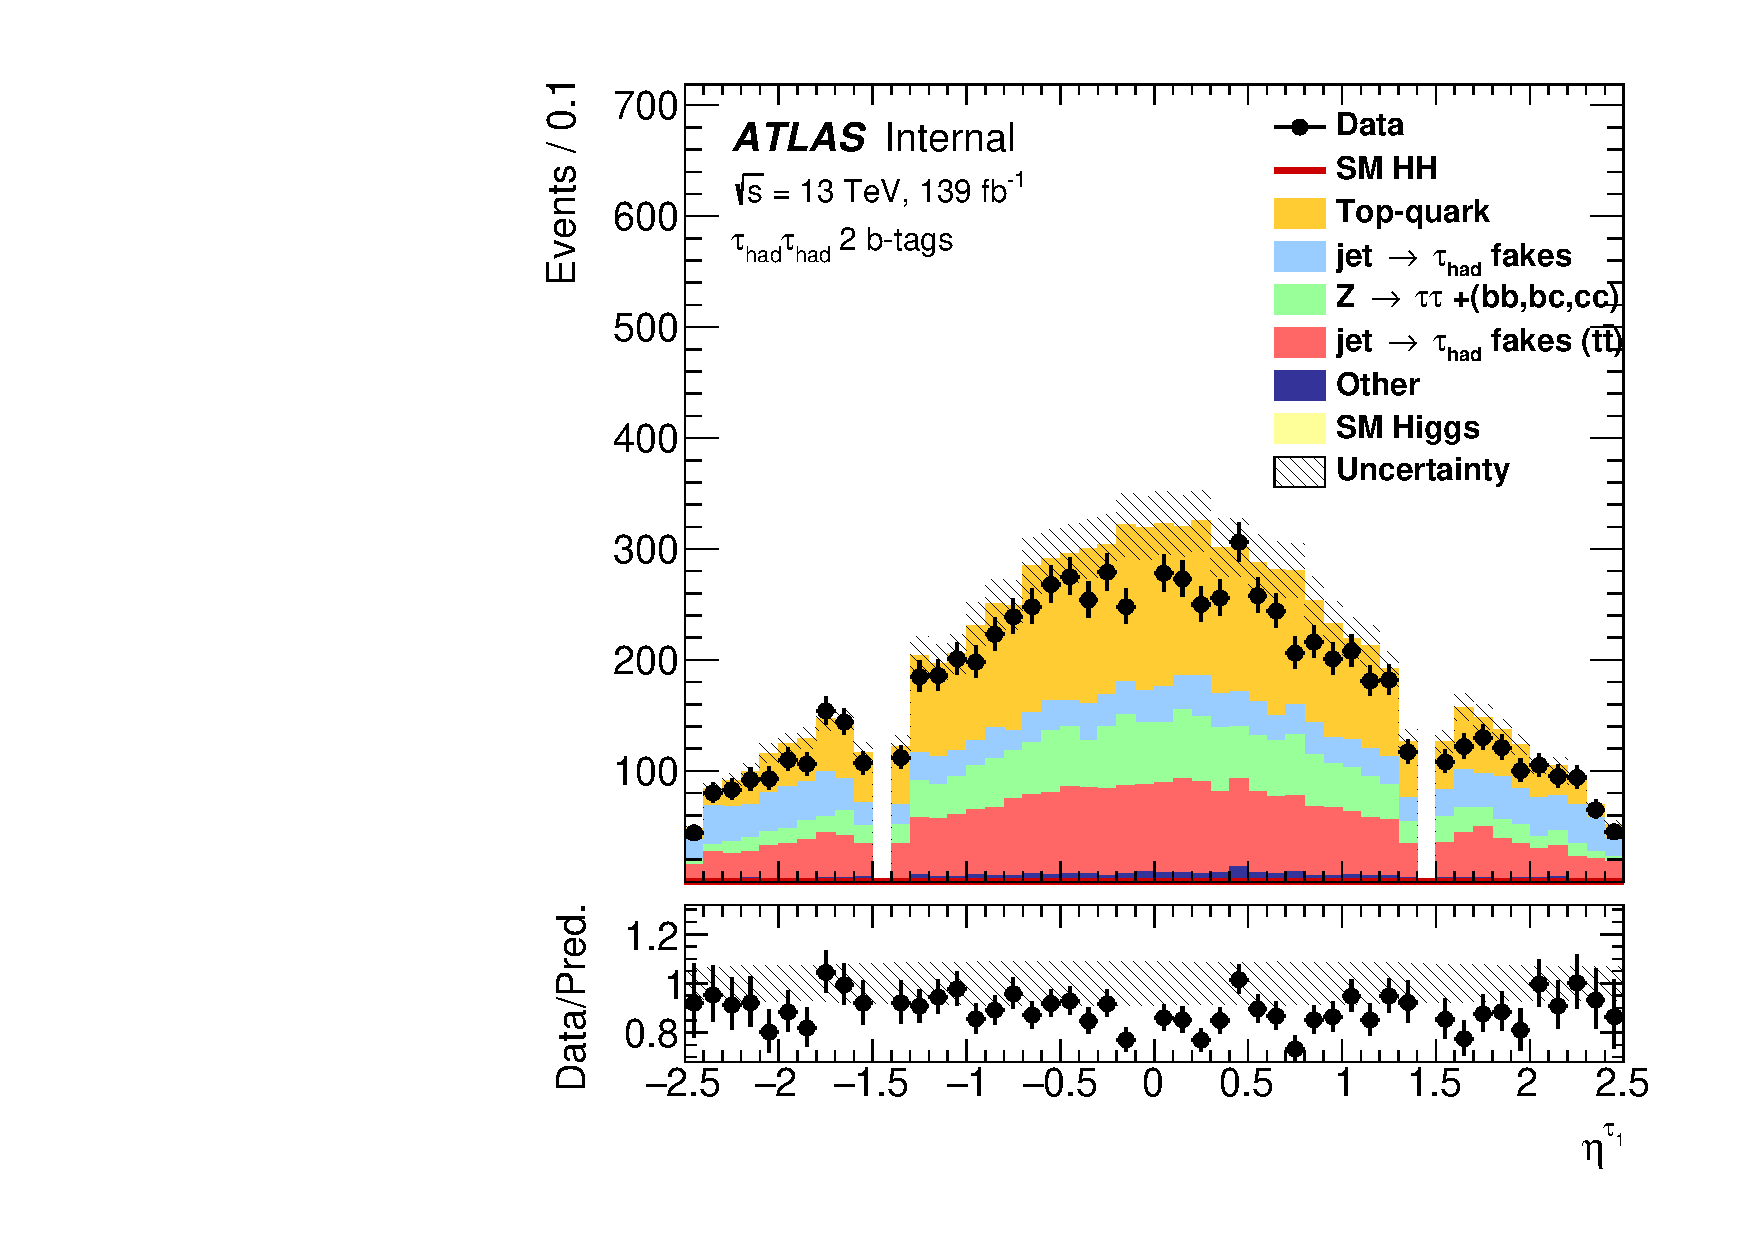
\includegraphics[width=.45\textwidth]{figures/selection/HadHad_HH/Region_BMin0_incJet1_distTau1Eta_J2_Y2015_DLLOS_T2_SpcTauHH_L0_Prefit.pdf}\\
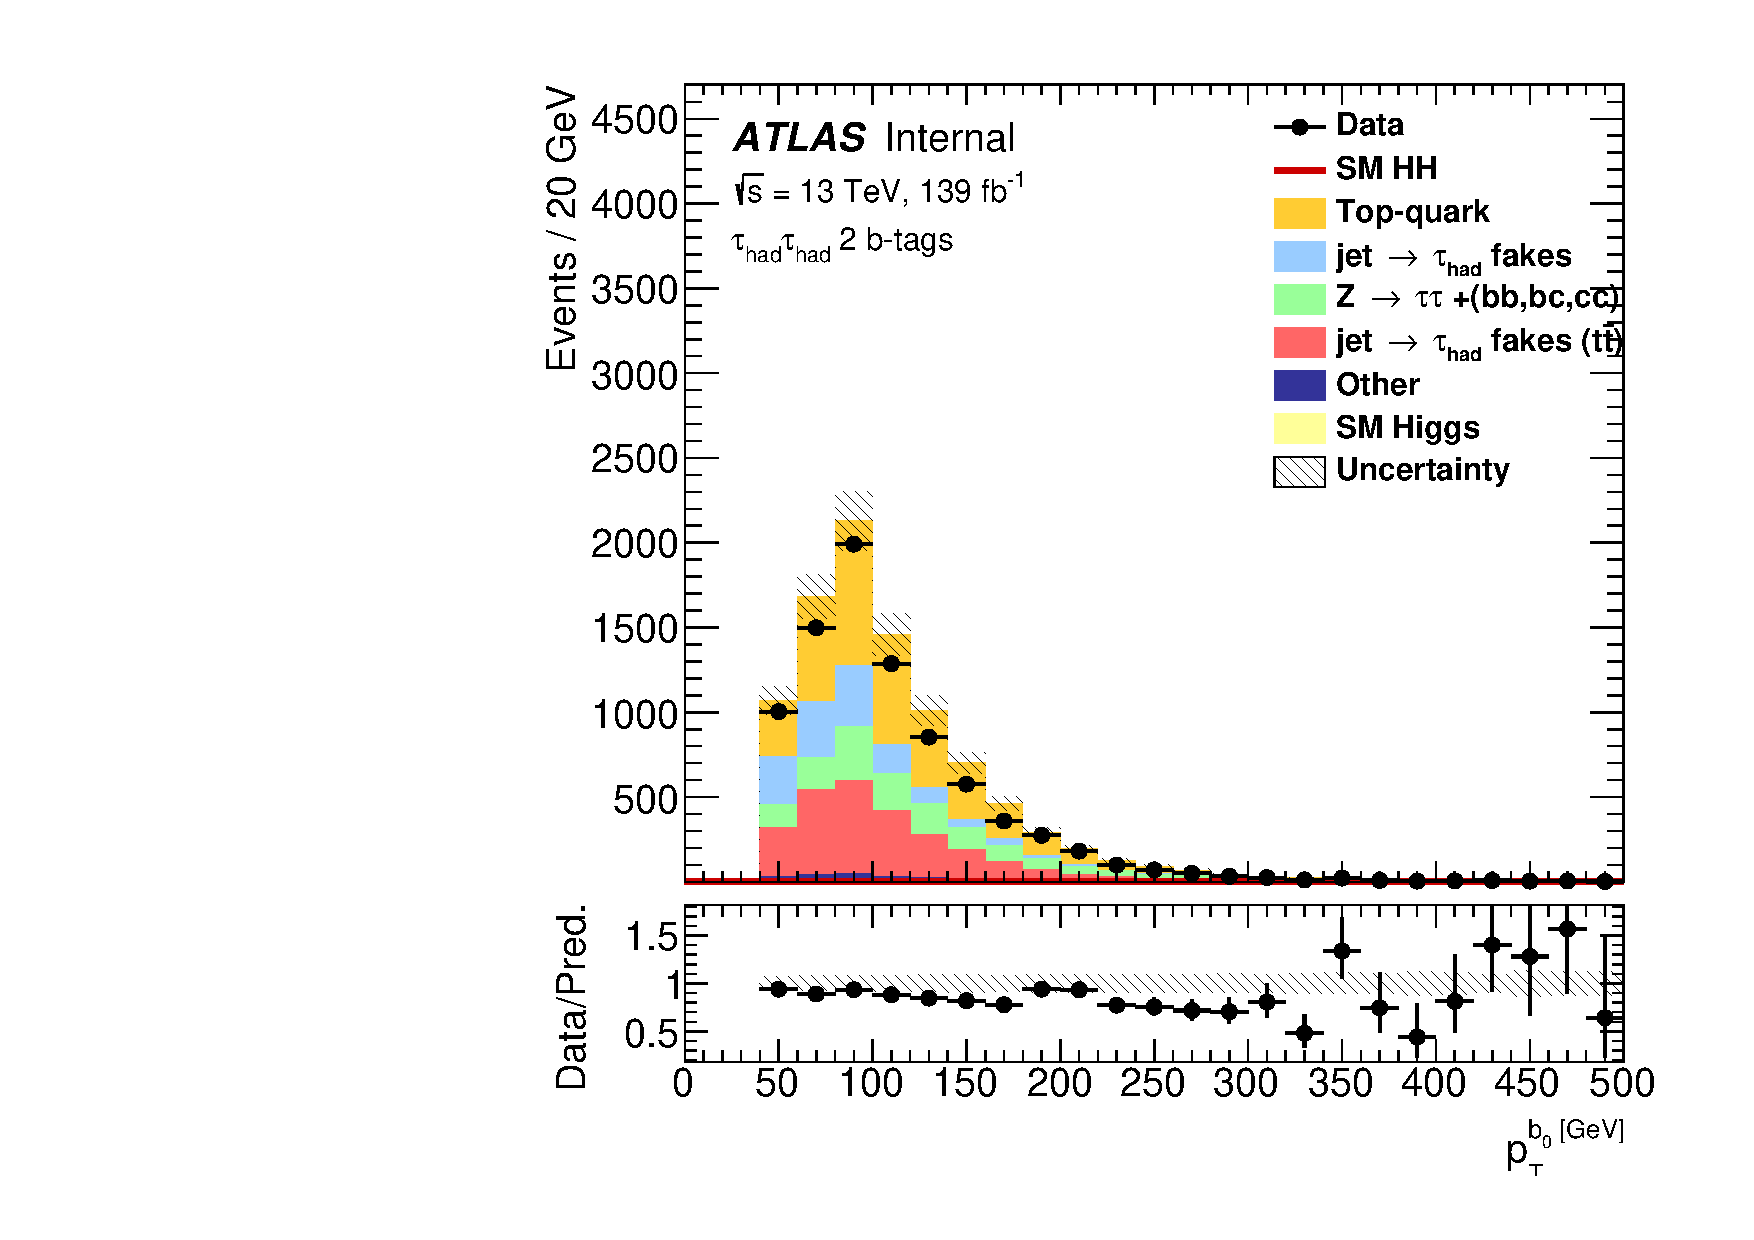
\includegraphics[width=.45\textwidth]{figures/selection/HadHad_HH/Region_BMin0_incJet1_distJet0Pt_J2_Y2015_DLLOS_T2_SpcTauHH_L0_Prefit.pdf}
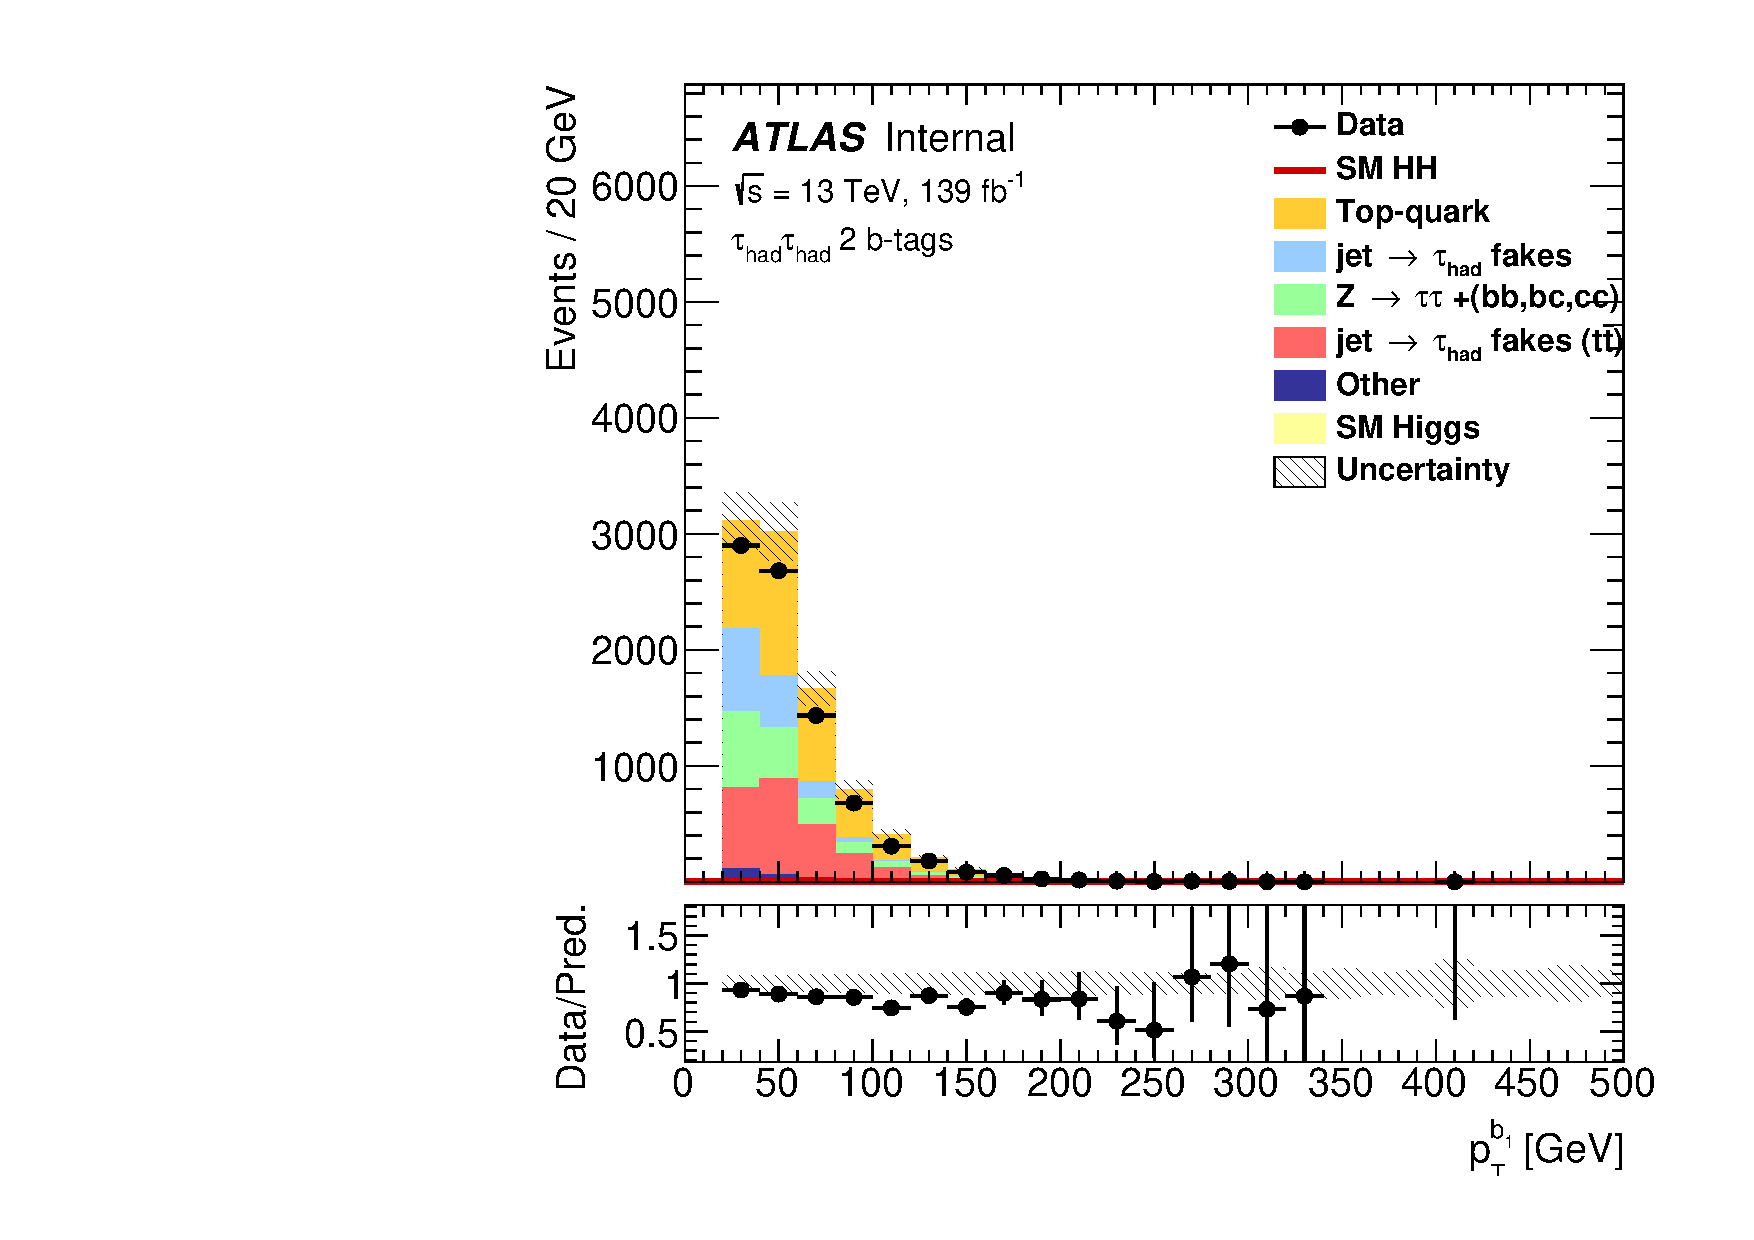
\includegraphics[width=.45\textwidth]{figures/selection/HadHad_HH/Region_BMin0_incJet1_distJet1Pt_J2_Y2015_DLLOS_T2_SpcTauHH_L0_Prefit.pdf}
\caption{Leading and sub-leading $\tau_{had}$ \pt and $\eta$ and $b$-jet \pt pre-fit
  distributions in the di-Higgs \hadhad signal region. (Inputs from 2021\_01\_15)}
\label{fig:HadHadPreselectionPtDistributions}
\end{figure}

\begin{figure}
\centering
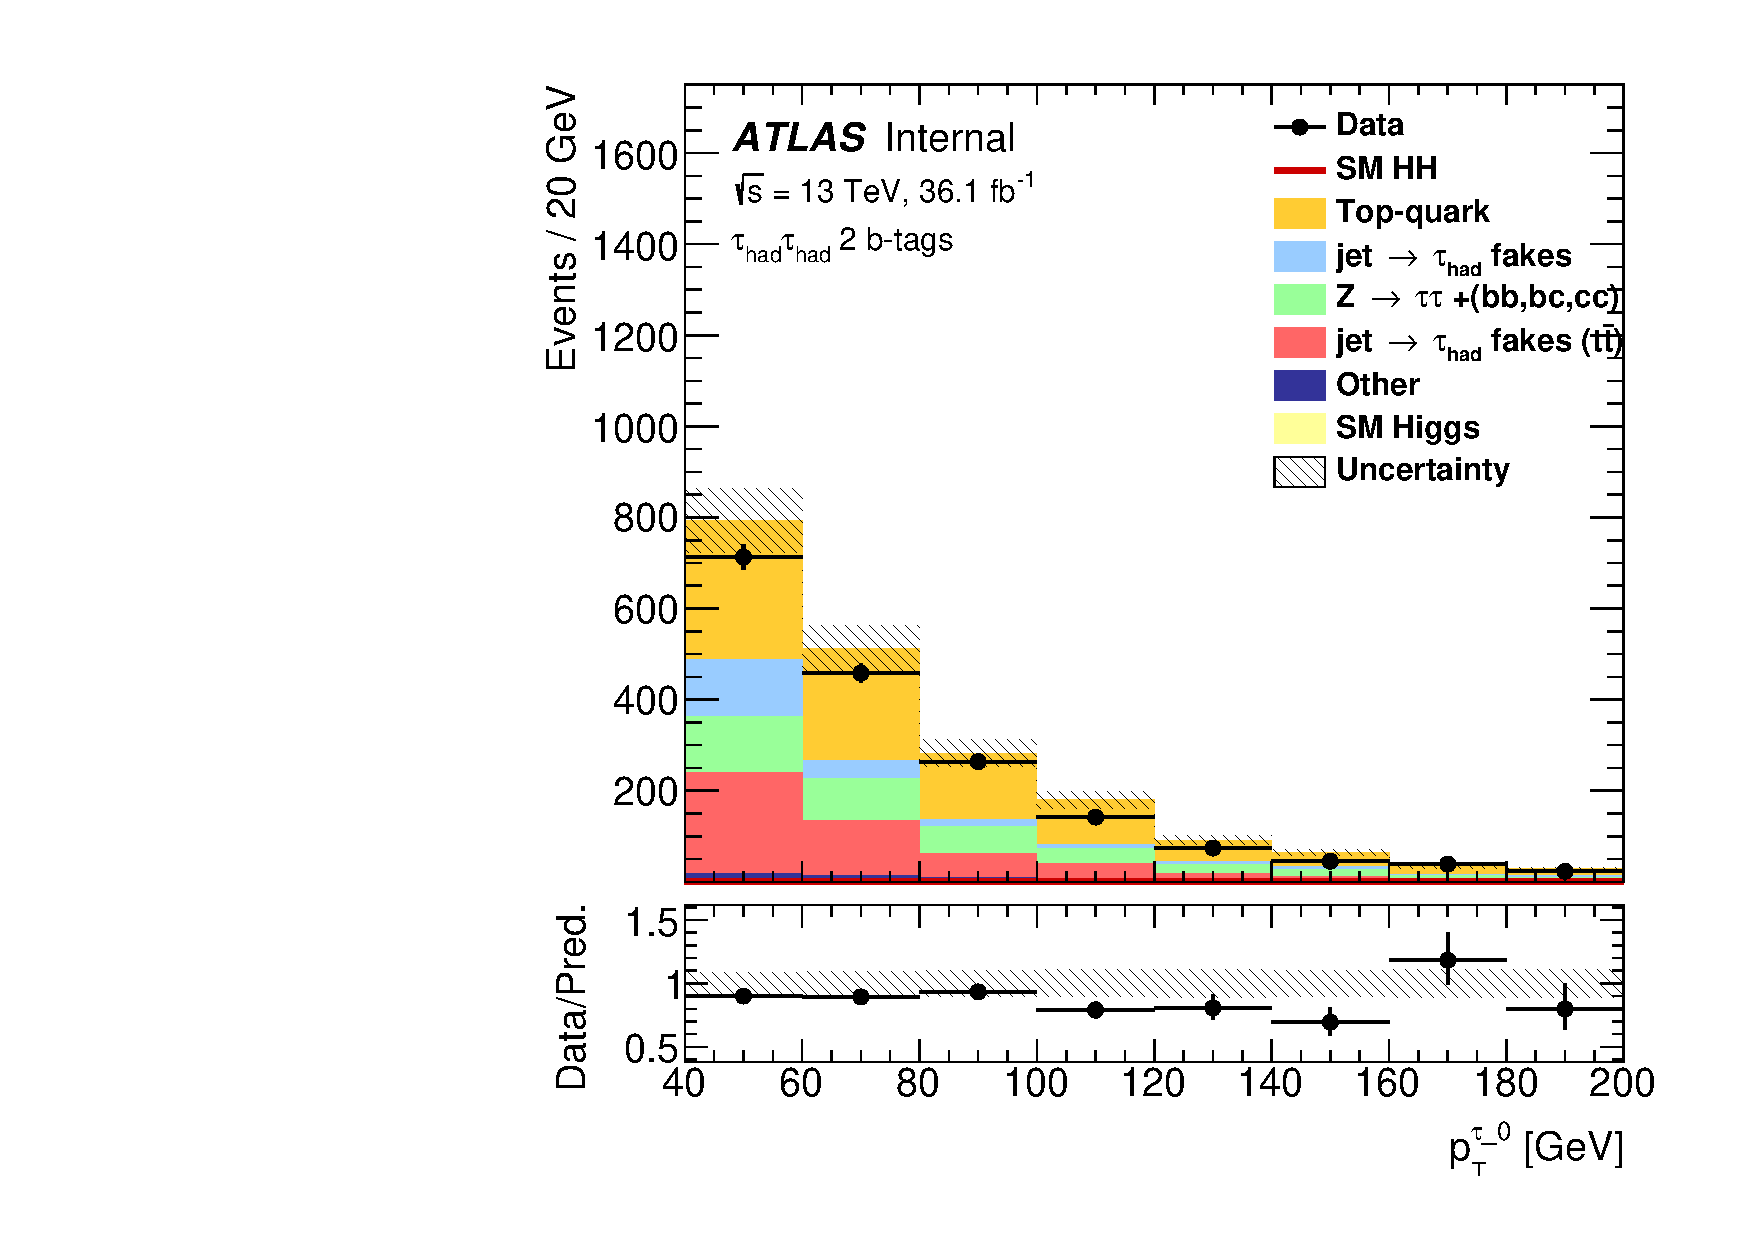
\includegraphics[width=.45\textwidth]{figures/selection/HadHad_HH/Plots2015/Region_BMin0_incJet1_distTau0Pt_J2_Y2015_DLLOS_T2_SpcTauHH_L0_Prefit.pdf}
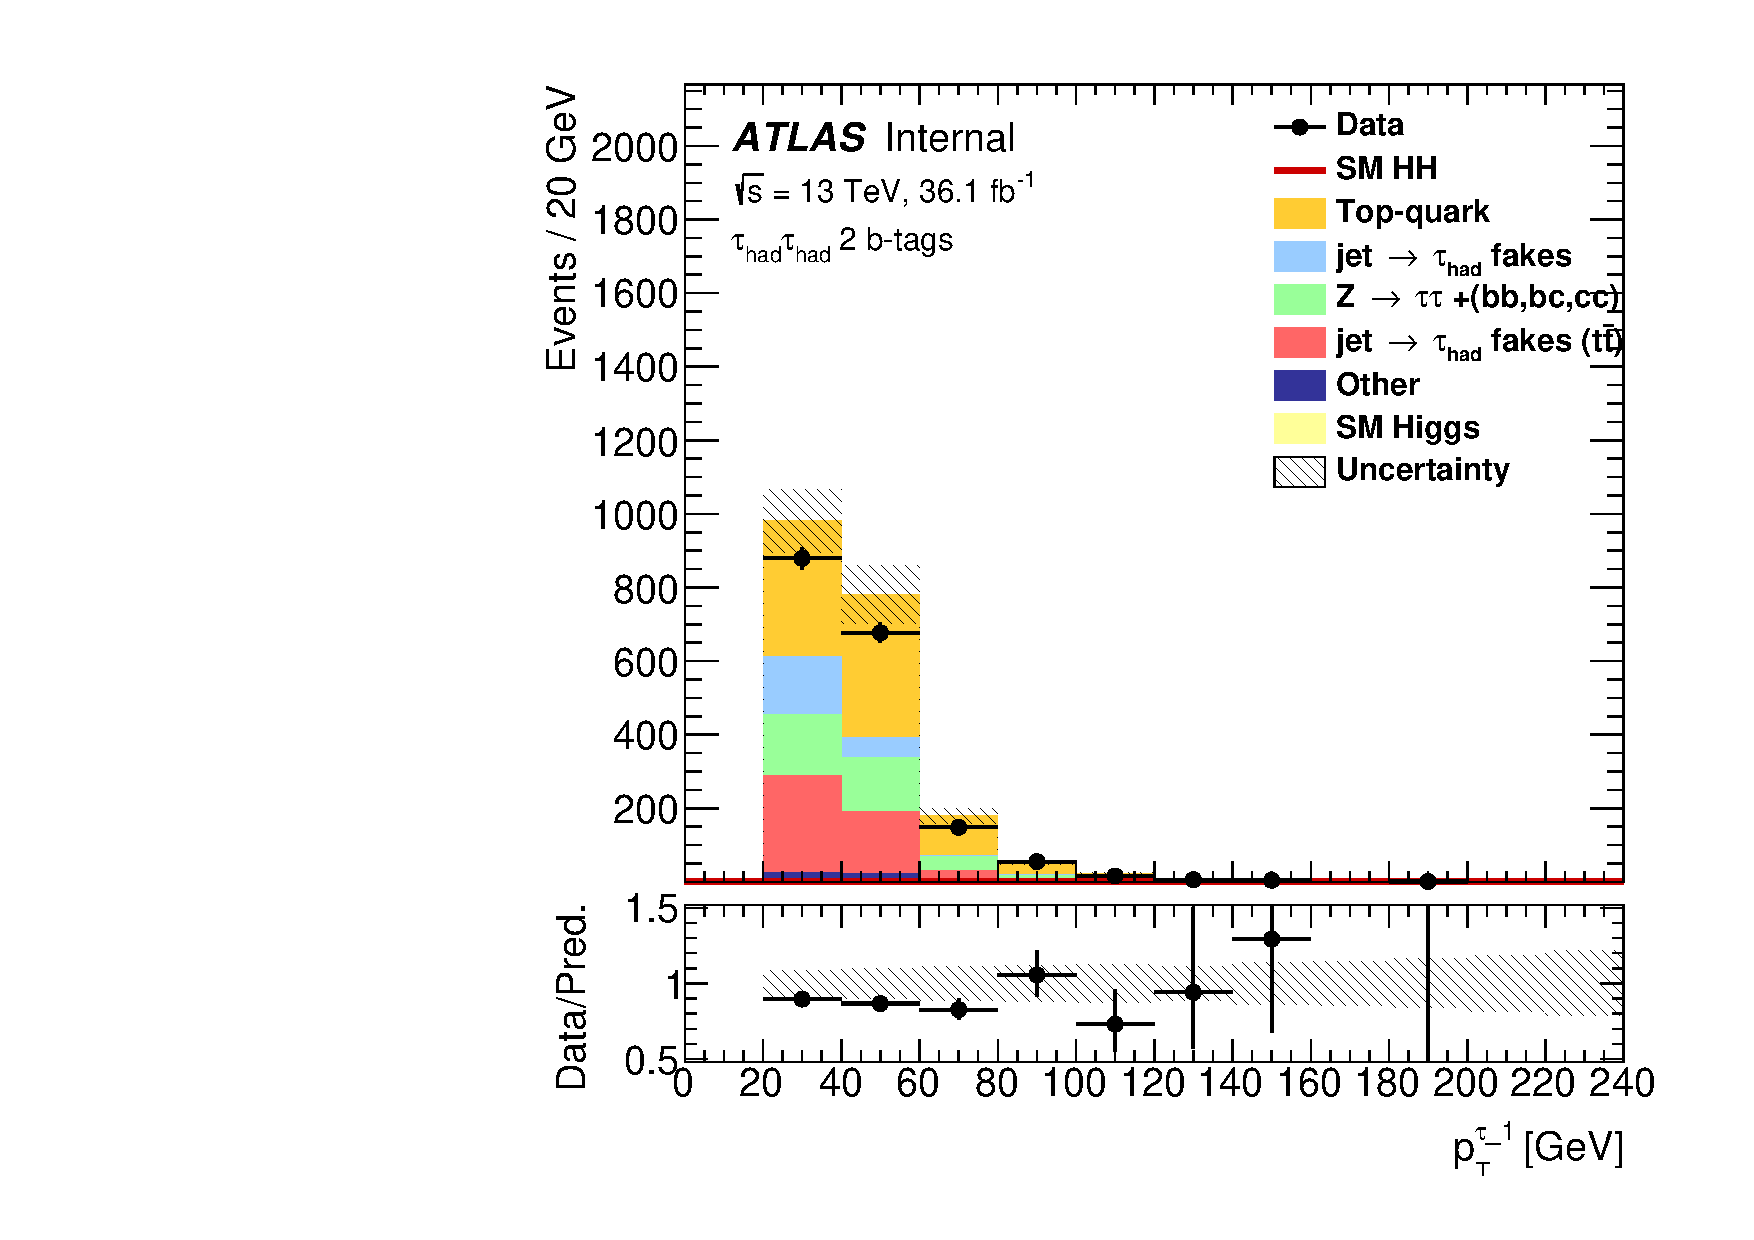
\includegraphics[width=.45\textwidth]{figures/selection/HadHad_HH/Plots2015/Region_BMin0_incJet1_distTau1Pt_J2_Y2015_DLLOS_T2_SpcTauHH_L0_Prefit.pdf}\\
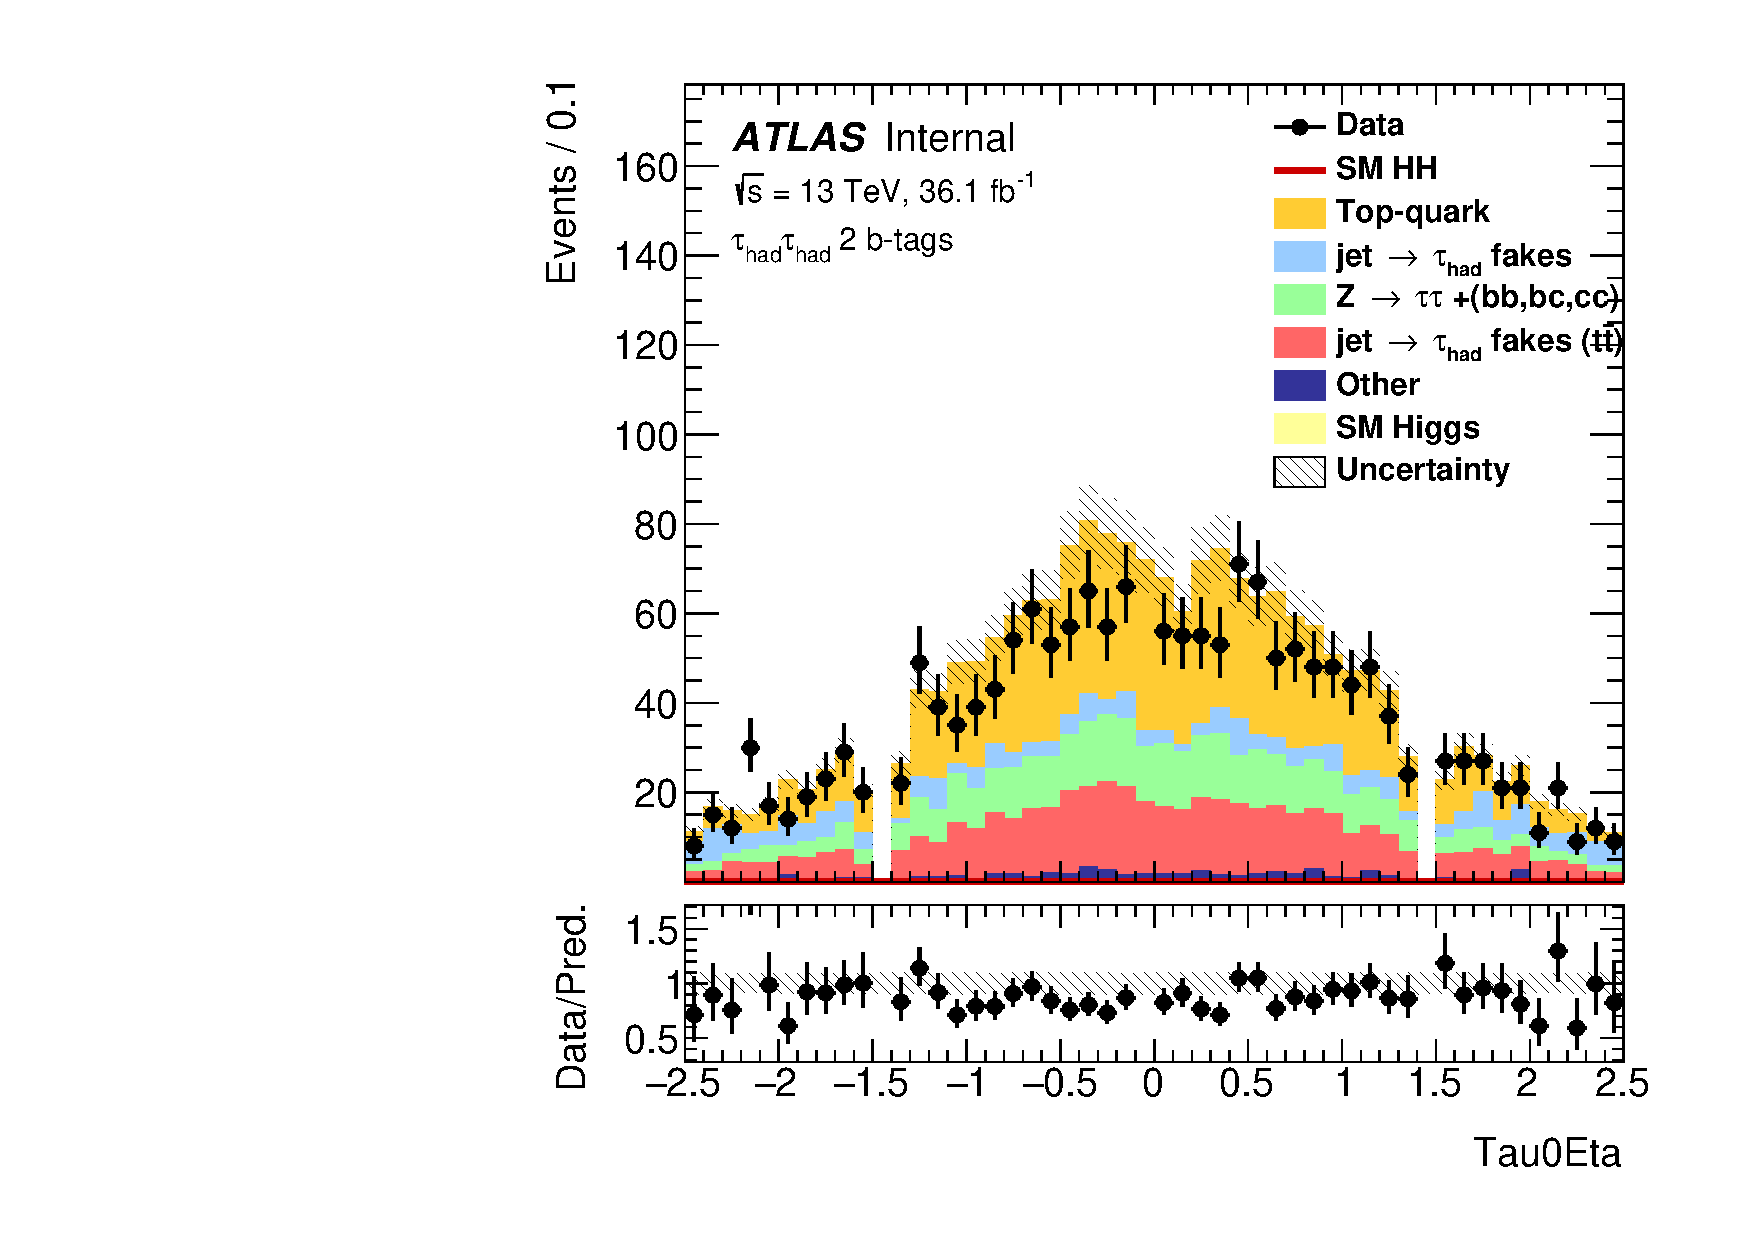
\includegraphics[width=.45\textwidth]{figures/selection/HadHad_HH/Plots2015/Region_BMin0_incJet1_distTau0Eta_J2_Y2015_DLLOS_T2_SpcTauHH_L0_Prefit.pdf}
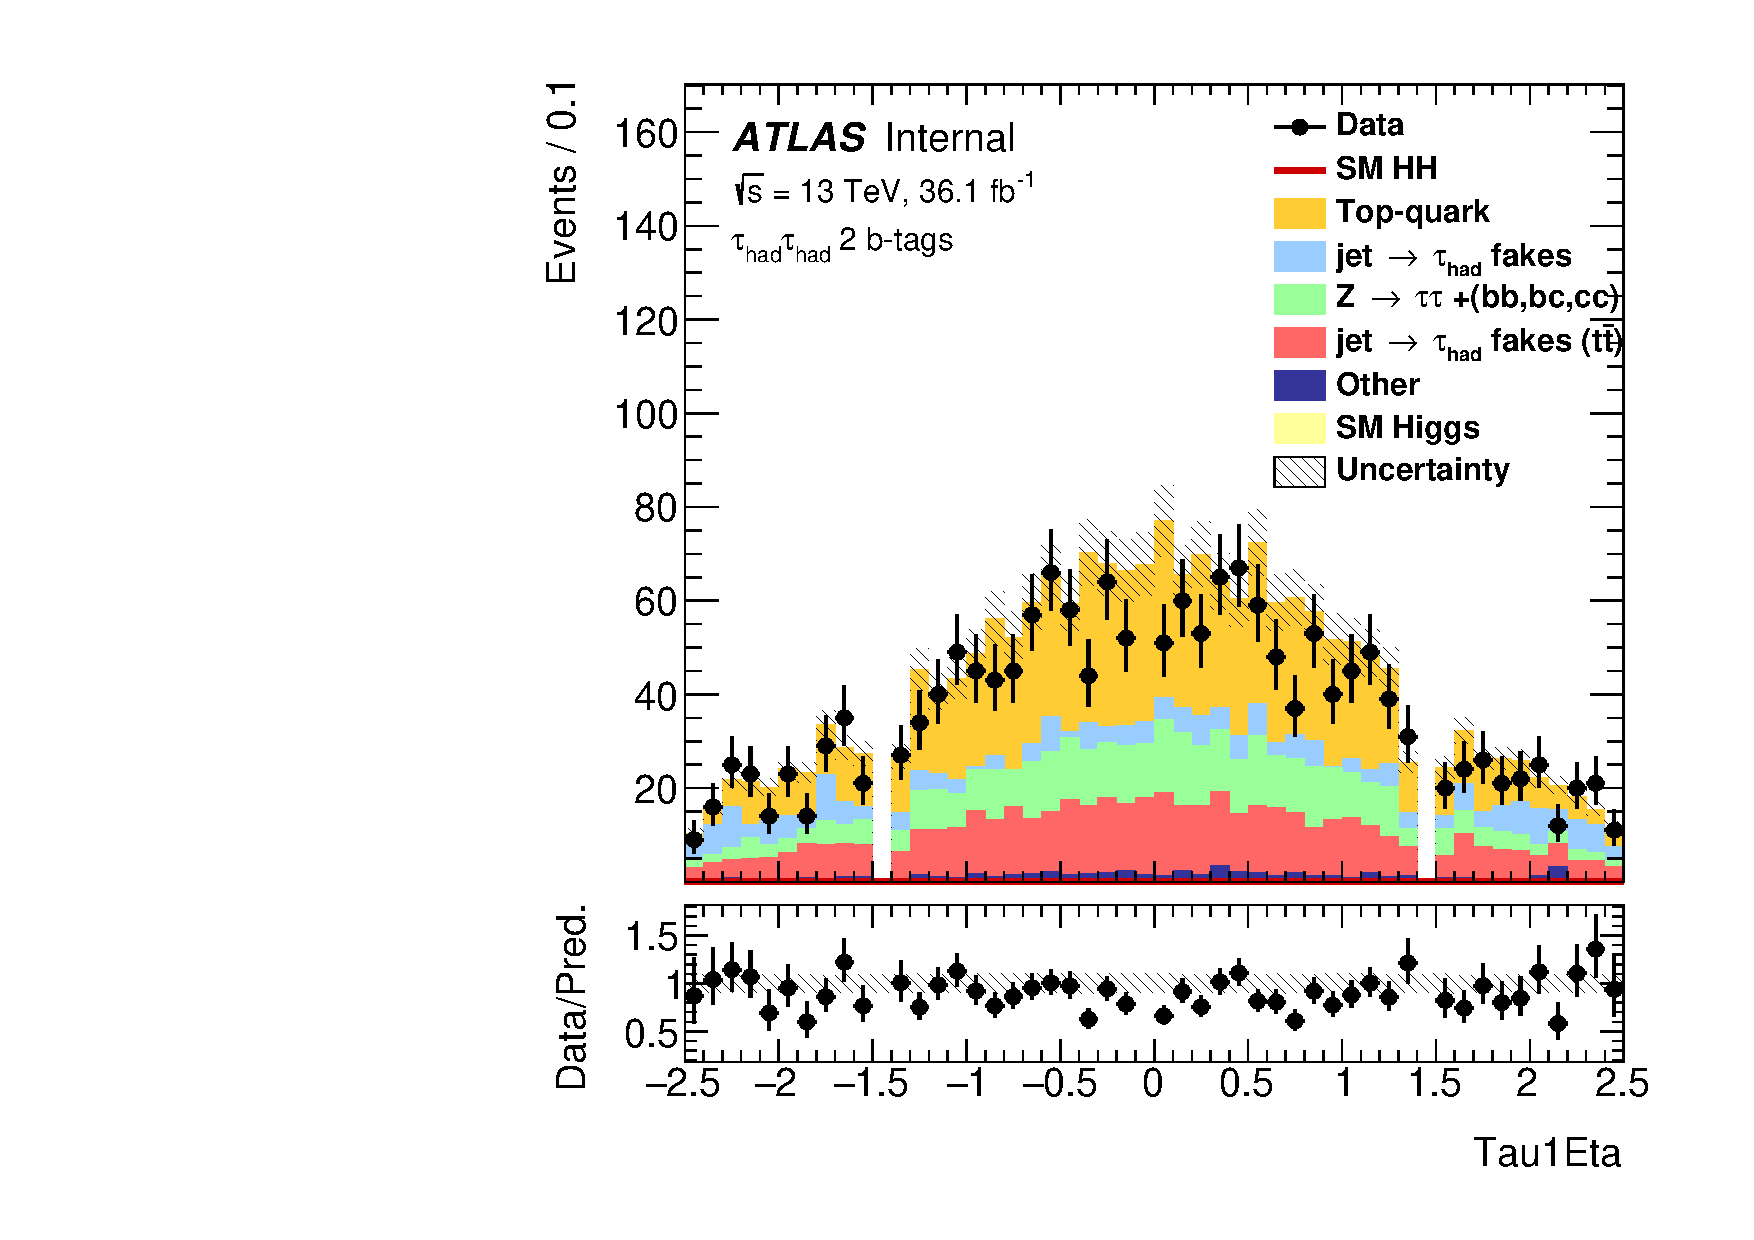
\includegraphics[width=.45\textwidth]{figures/selection/HadHad_HH/Plots2015/Region_BMin0_incJet1_distTau1Eta_J2_Y2015_DLLOS_T2_SpcTauHH_L0_Prefit.pdf}\\
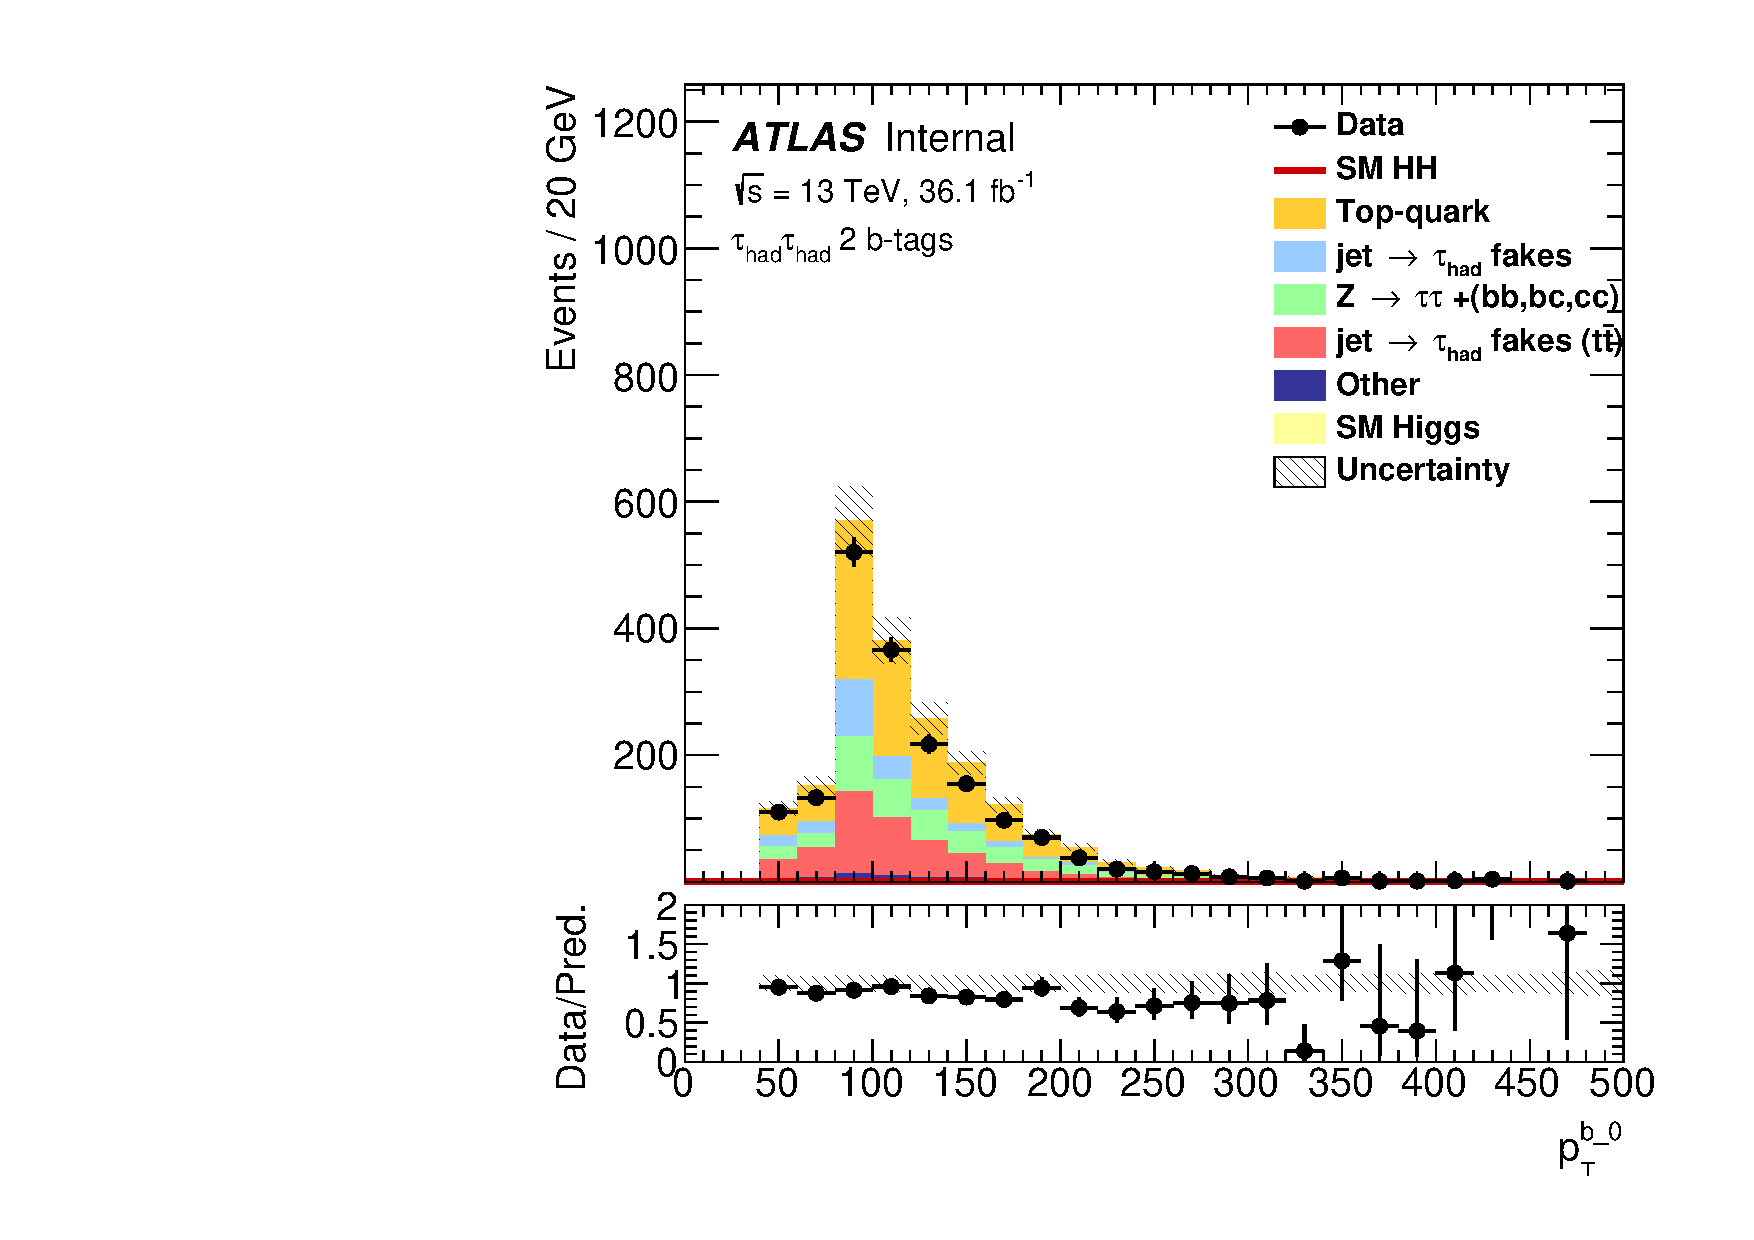
\includegraphics[width=.45\textwidth]{figures/selection/HadHad_HH/Plots2015/Region_BMin0_incJet1_distJet0Pt_J2_Y2015_DLLOS_T2_SpcTauHH_L0_Prefit.pdf}
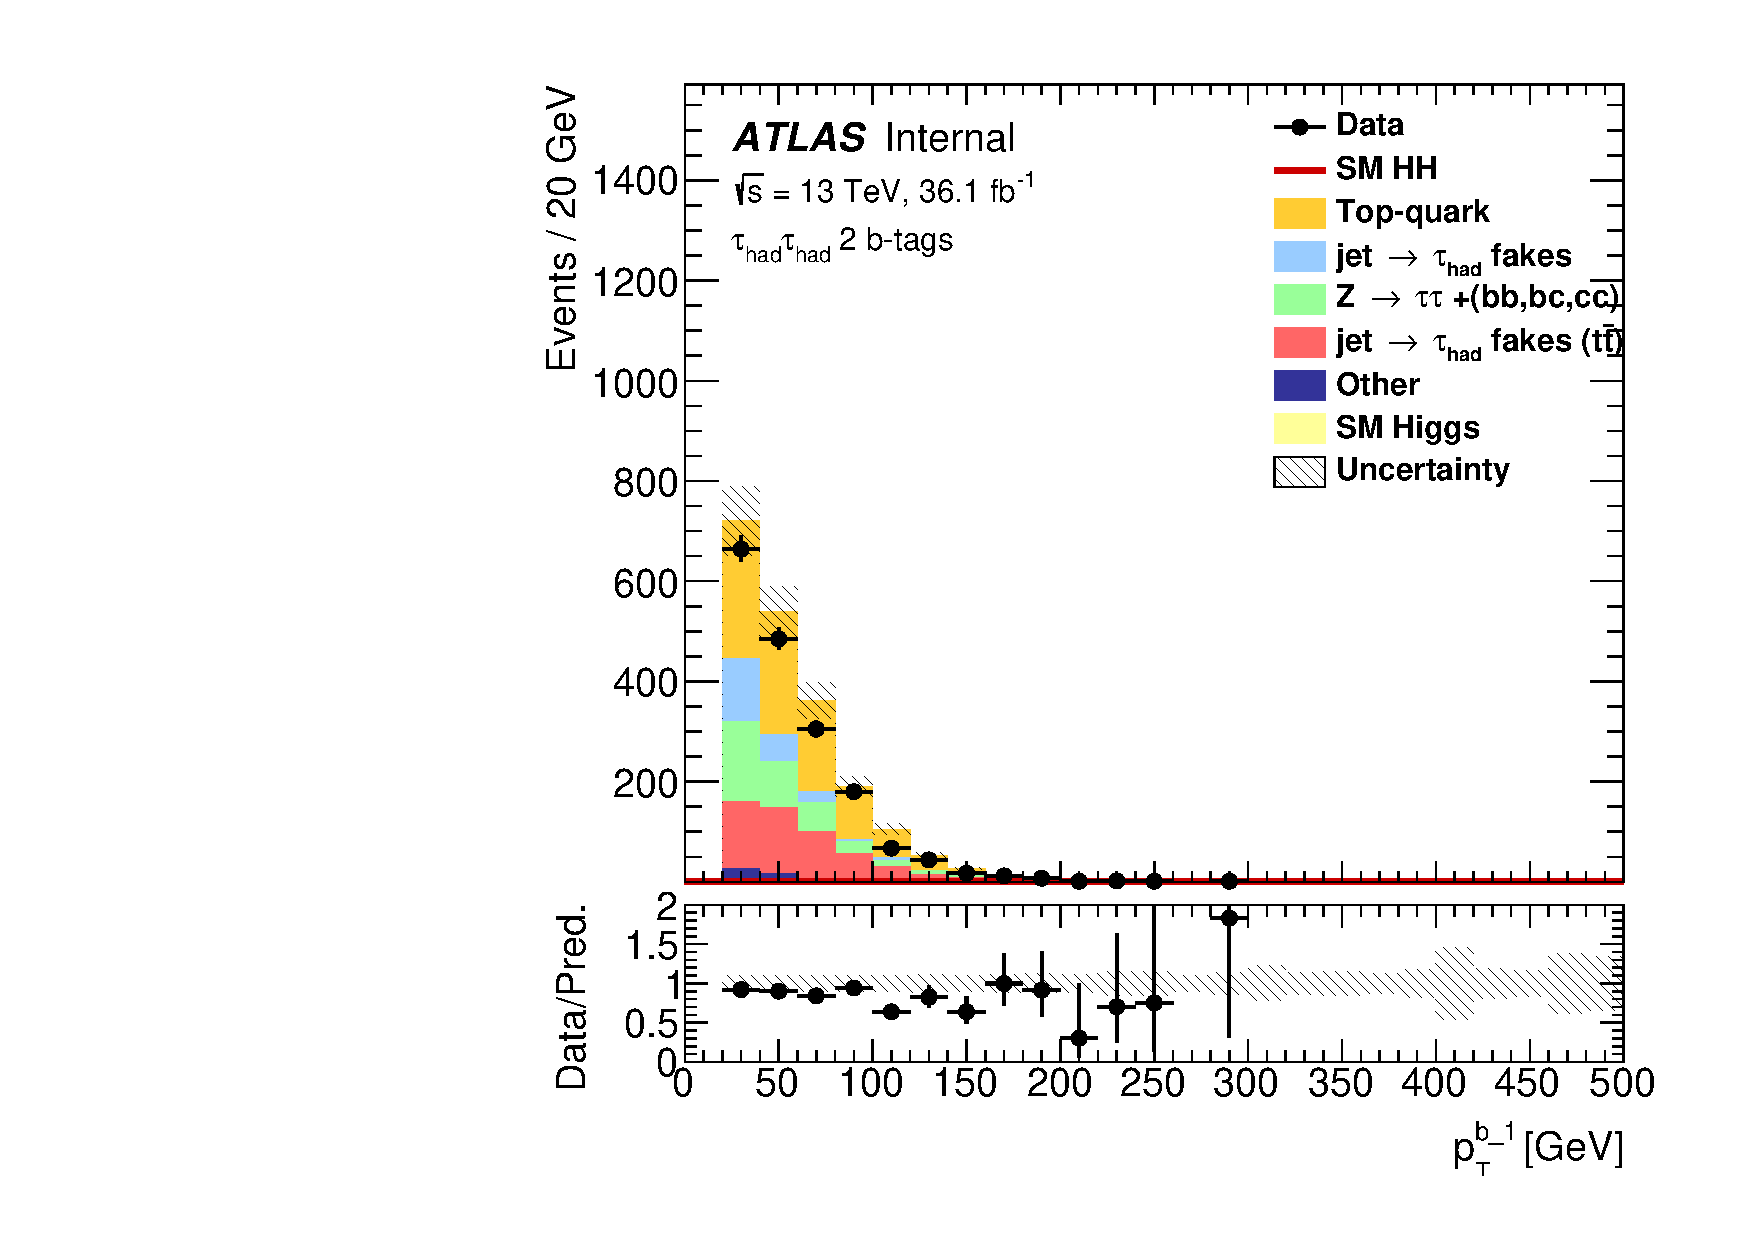
\includegraphics[width=.45\textwidth]{figures/selection/HadHad_HH/Plots2015/Region_BMin0_incJet1_distJet1Pt_J2_Y2015_DLLOS_T2_SpcTauHH_L0_Prefit.pdf}
\caption{Leading and sub-leading $\tau_{had}$ \pt and $\eta$ and $b$-jet \pt pre-fit
  distributions in the di-Higgs \hadhad signal region for the 2015-2016 data-taking period. (Inputs from 2021\_01\_15)}
\label{fig:HadHadPreselectionPtDistributions2015}
\end{figure}

\begin{figure}
\centering
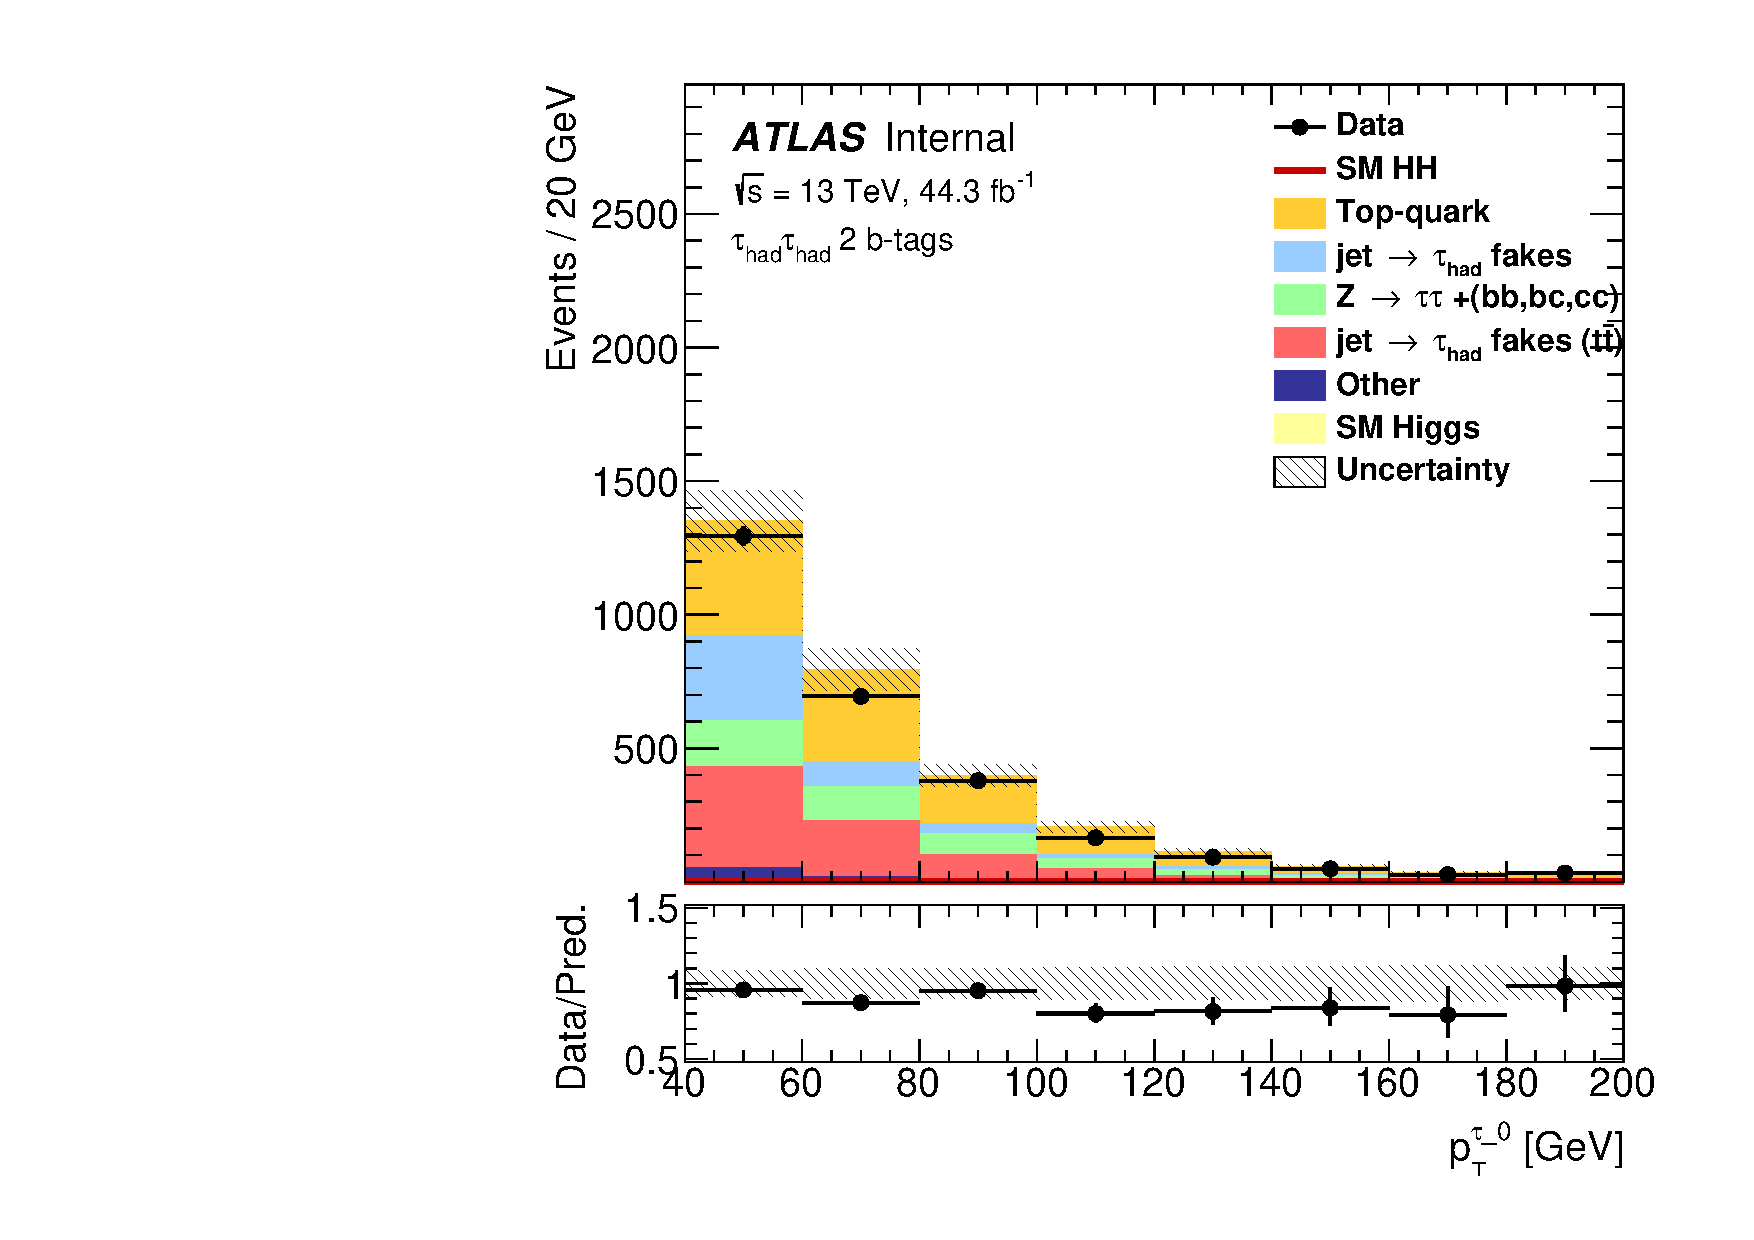
\includegraphics[width=.45\textwidth]{figures/selection/HadHad_HH/Plots2017/Region_BMin0_incJet1_distTau0Pt_J2_Y2015_DLLOS_T2_SpcTauHH_L0_Prefit.pdf}
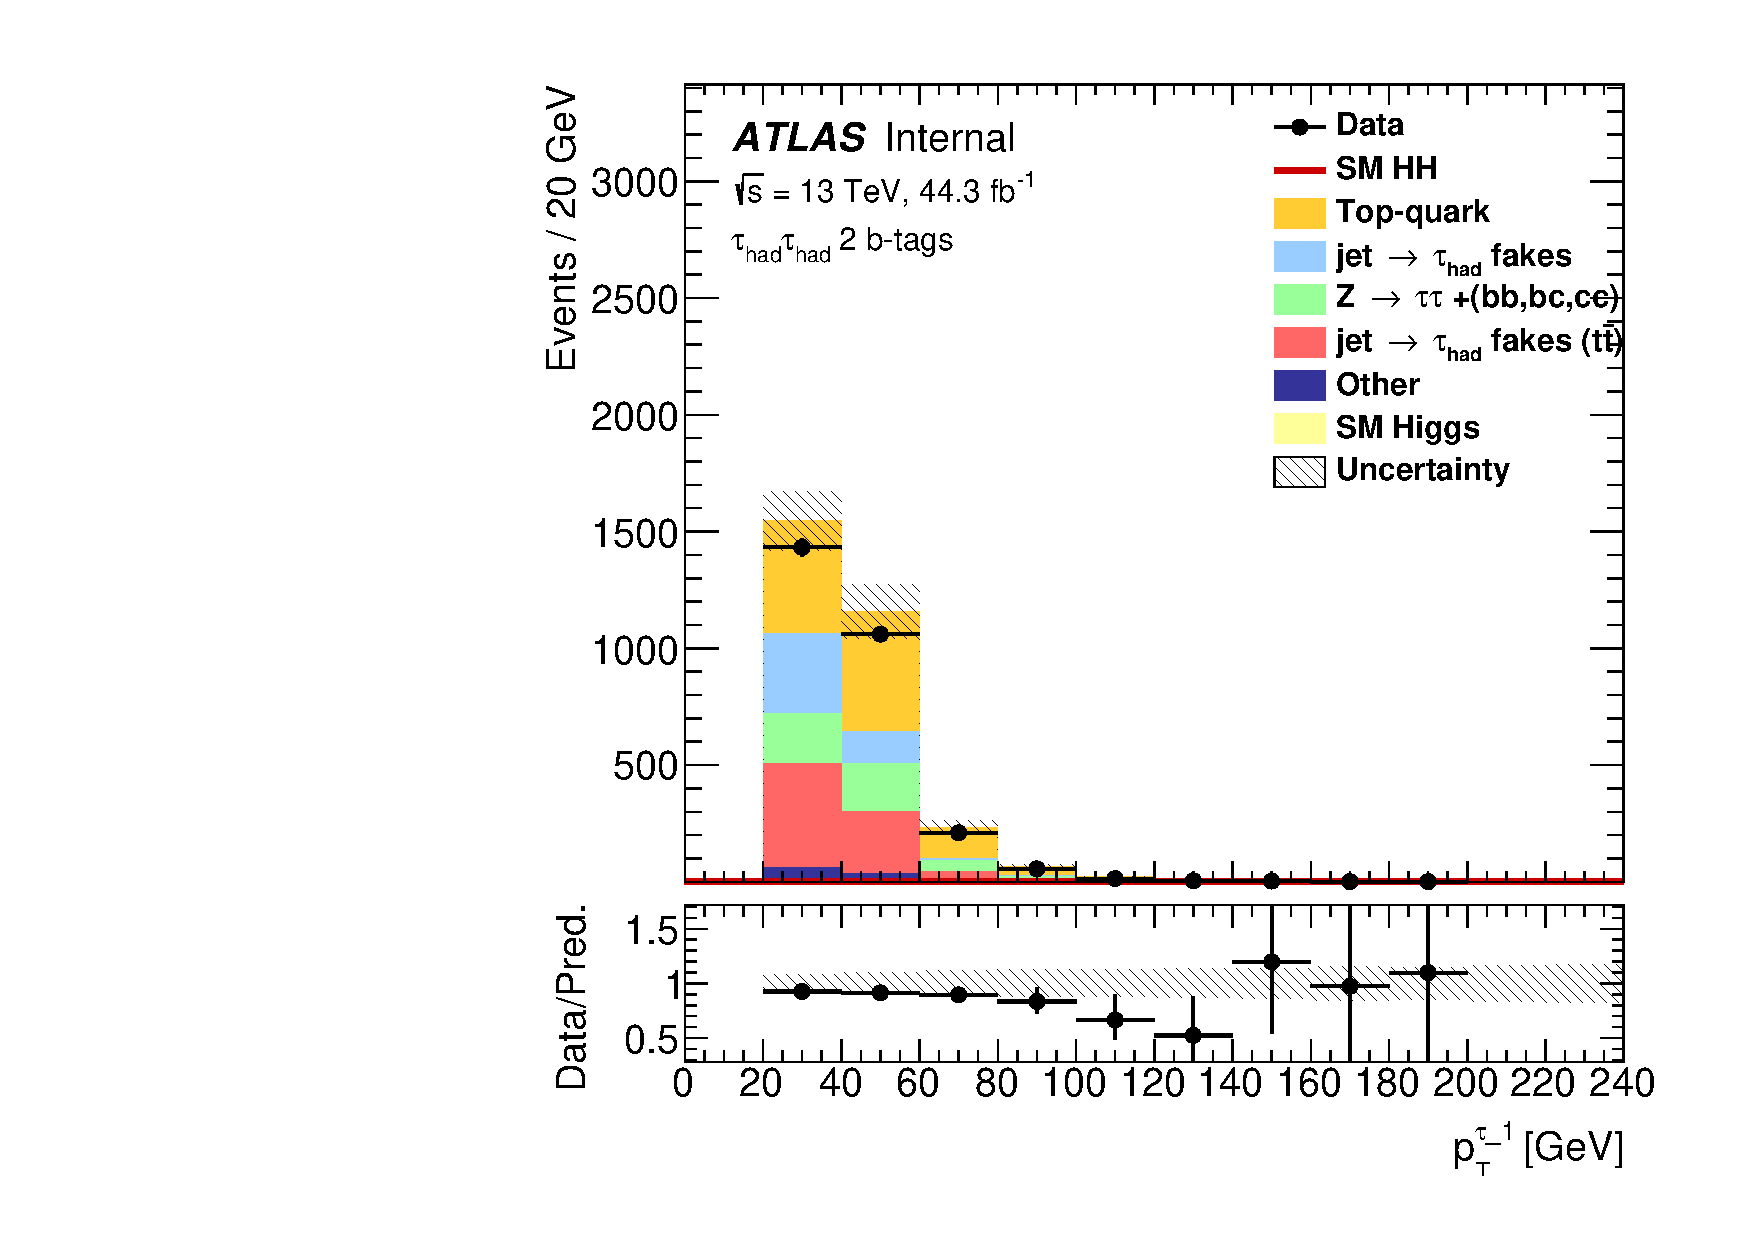
\includegraphics[width=.45\textwidth]{figures/selection/HadHad_HH/Plots2017/Region_BMin0_incJet1_distTau1Pt_J2_Y2015_DLLOS_T2_SpcTauHH_L0_Prefit.pdf}\\
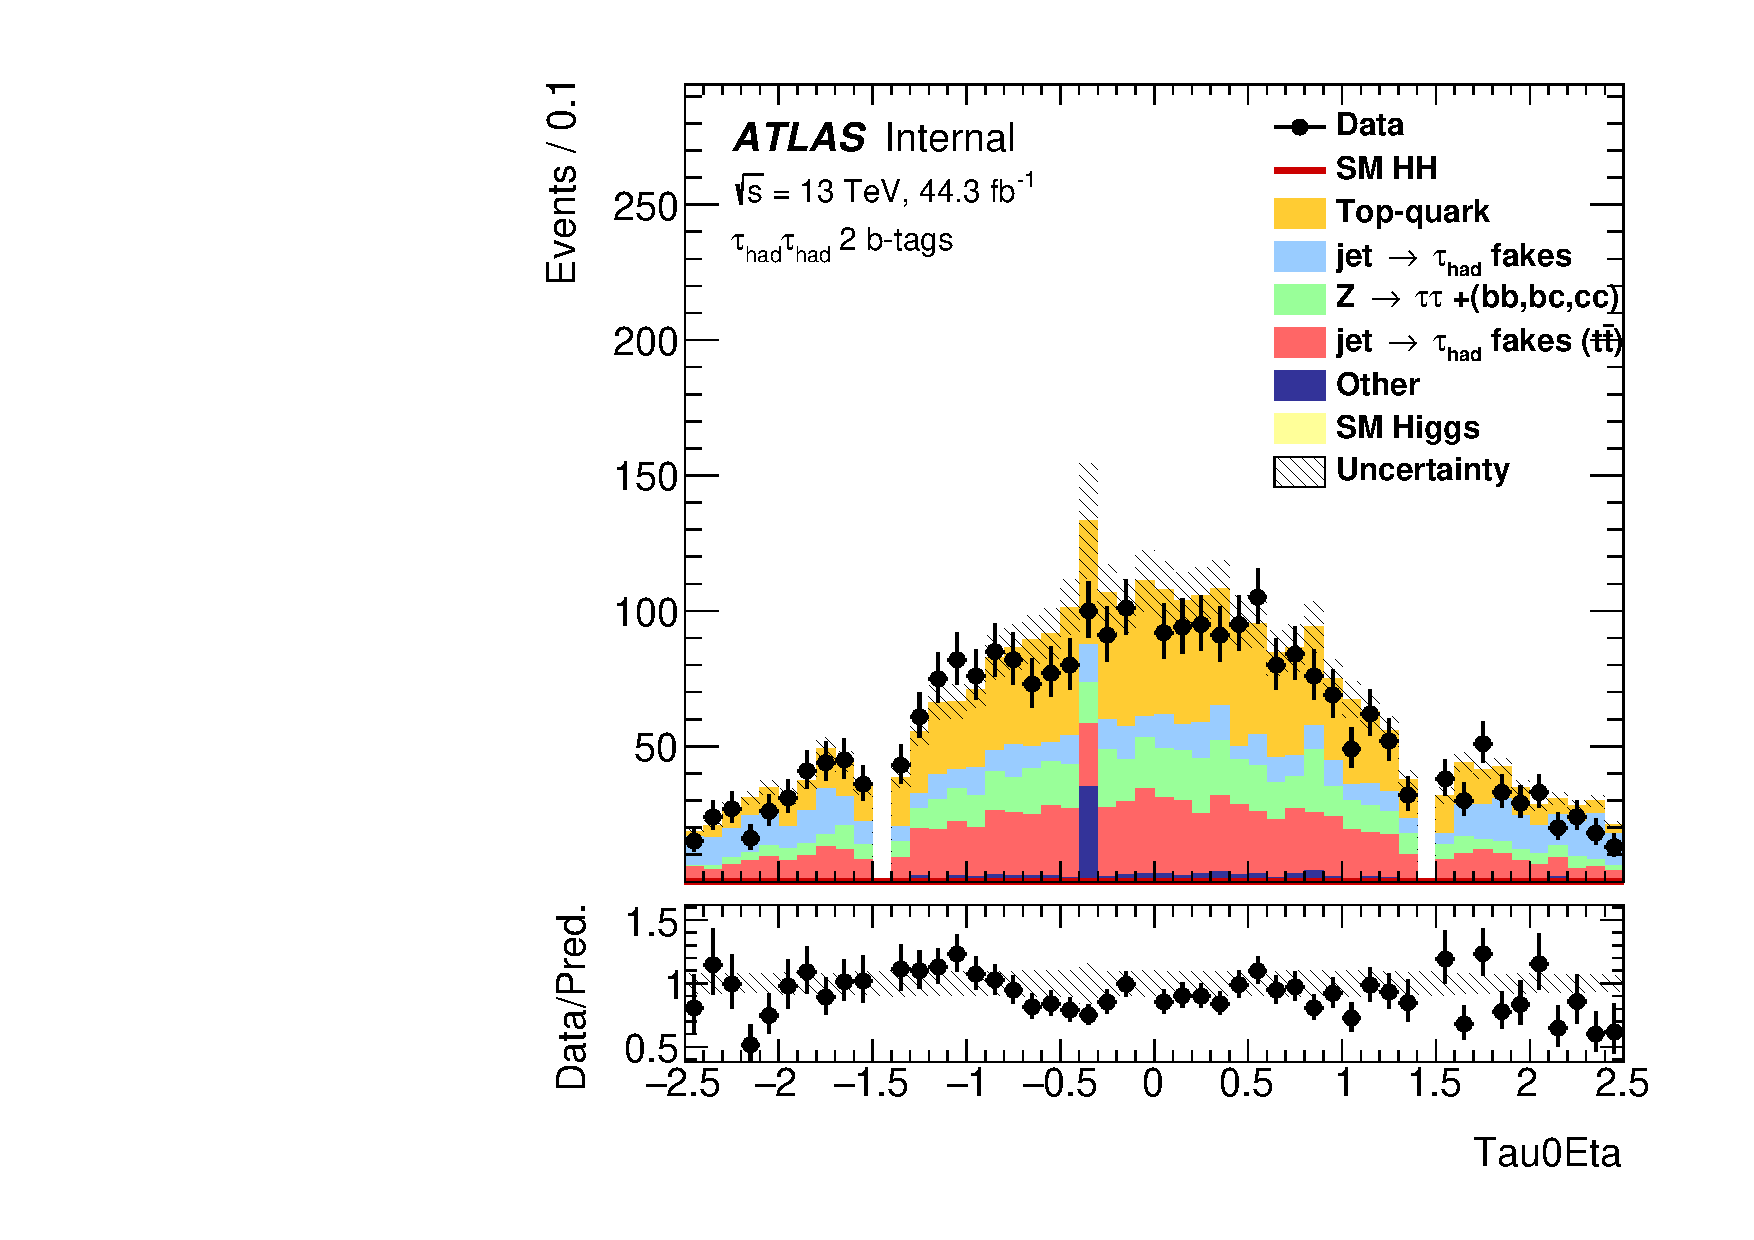
\includegraphics[width=.45\textwidth]{figures/selection/HadHad_HH/Plots2017/Region_BMin0_incJet1_distTau0Eta_J2_Y2015_DLLOS_T2_SpcTauHH_L0_Prefit.pdf}
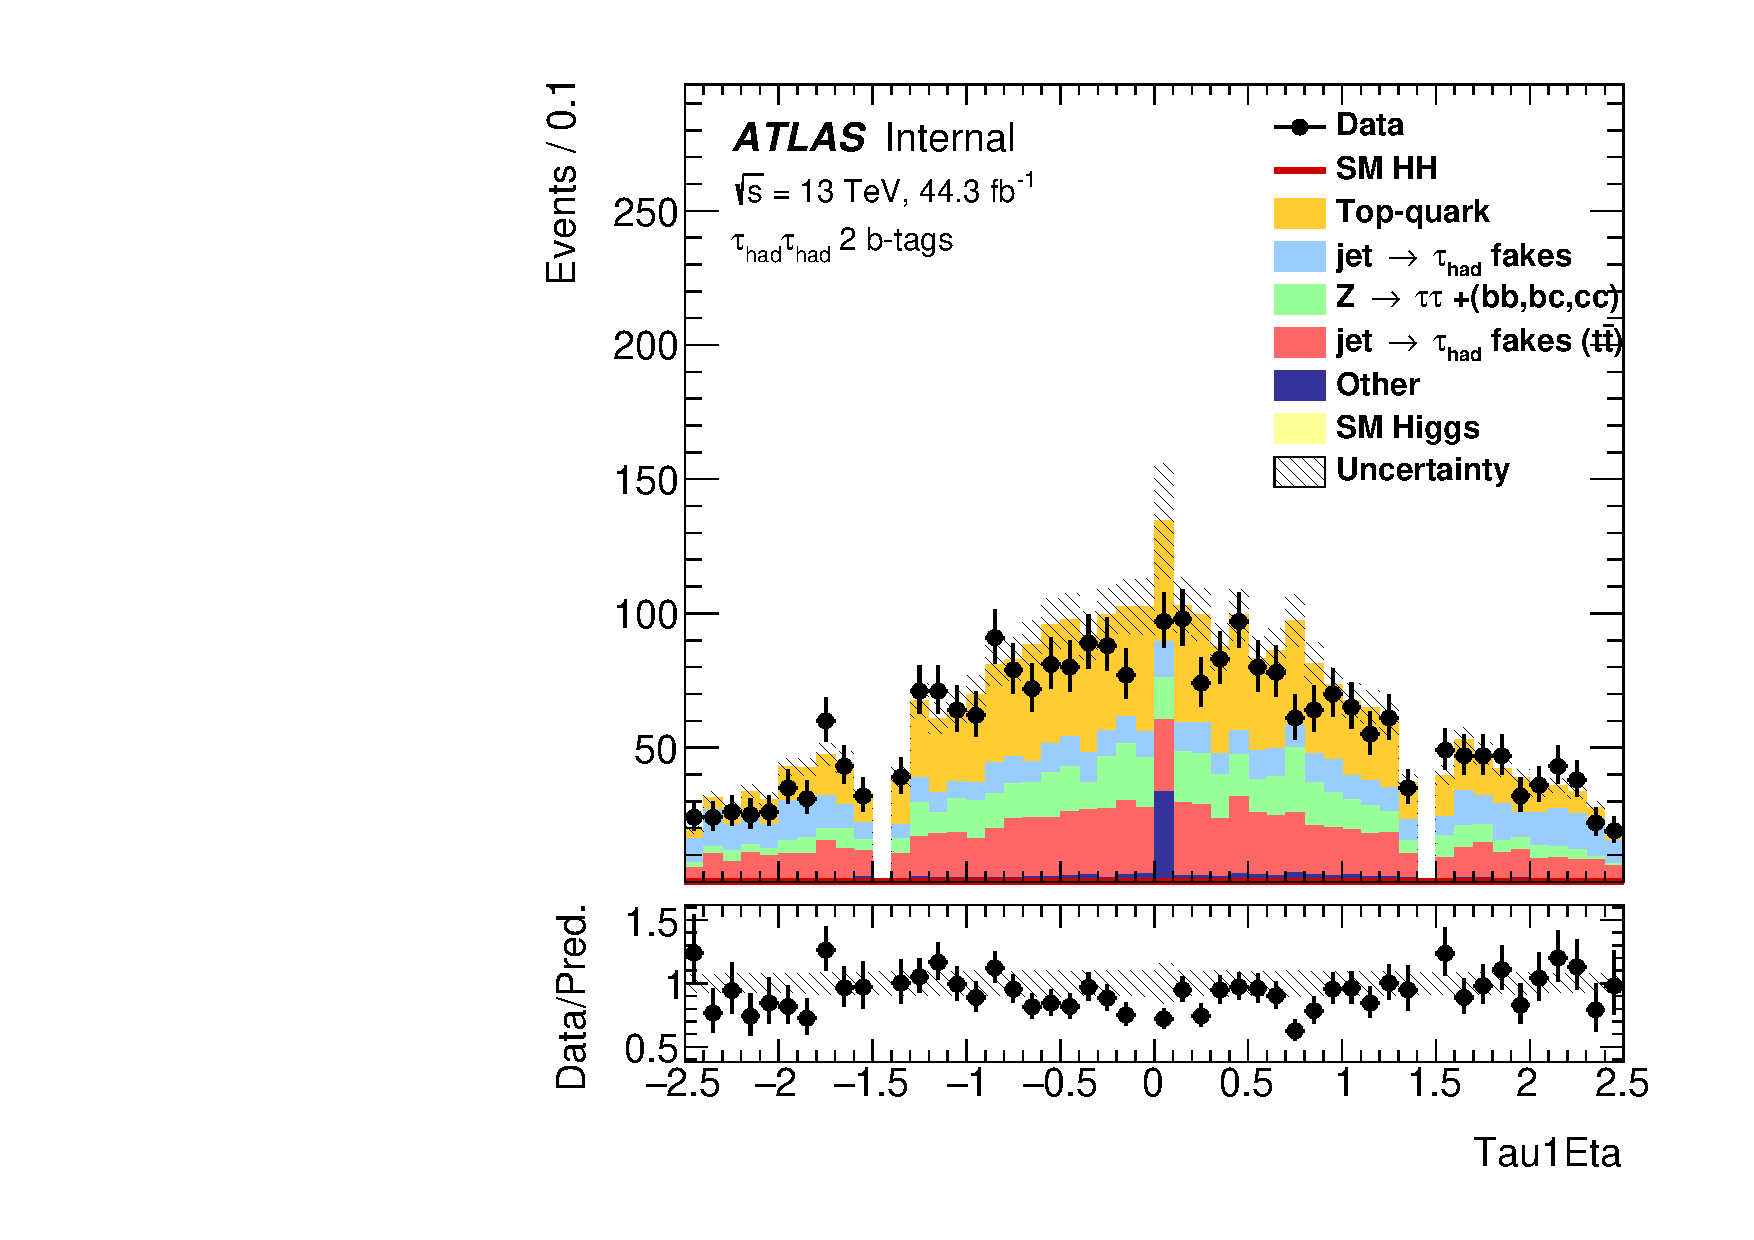
\includegraphics[width=.45\textwidth]{figures/selection/HadHad_HH/Plots2017/Region_BMin0_incJet1_distTau1Eta_J2_Y2015_DLLOS_T2_SpcTauHH_L0_Prefit.pdf}\\
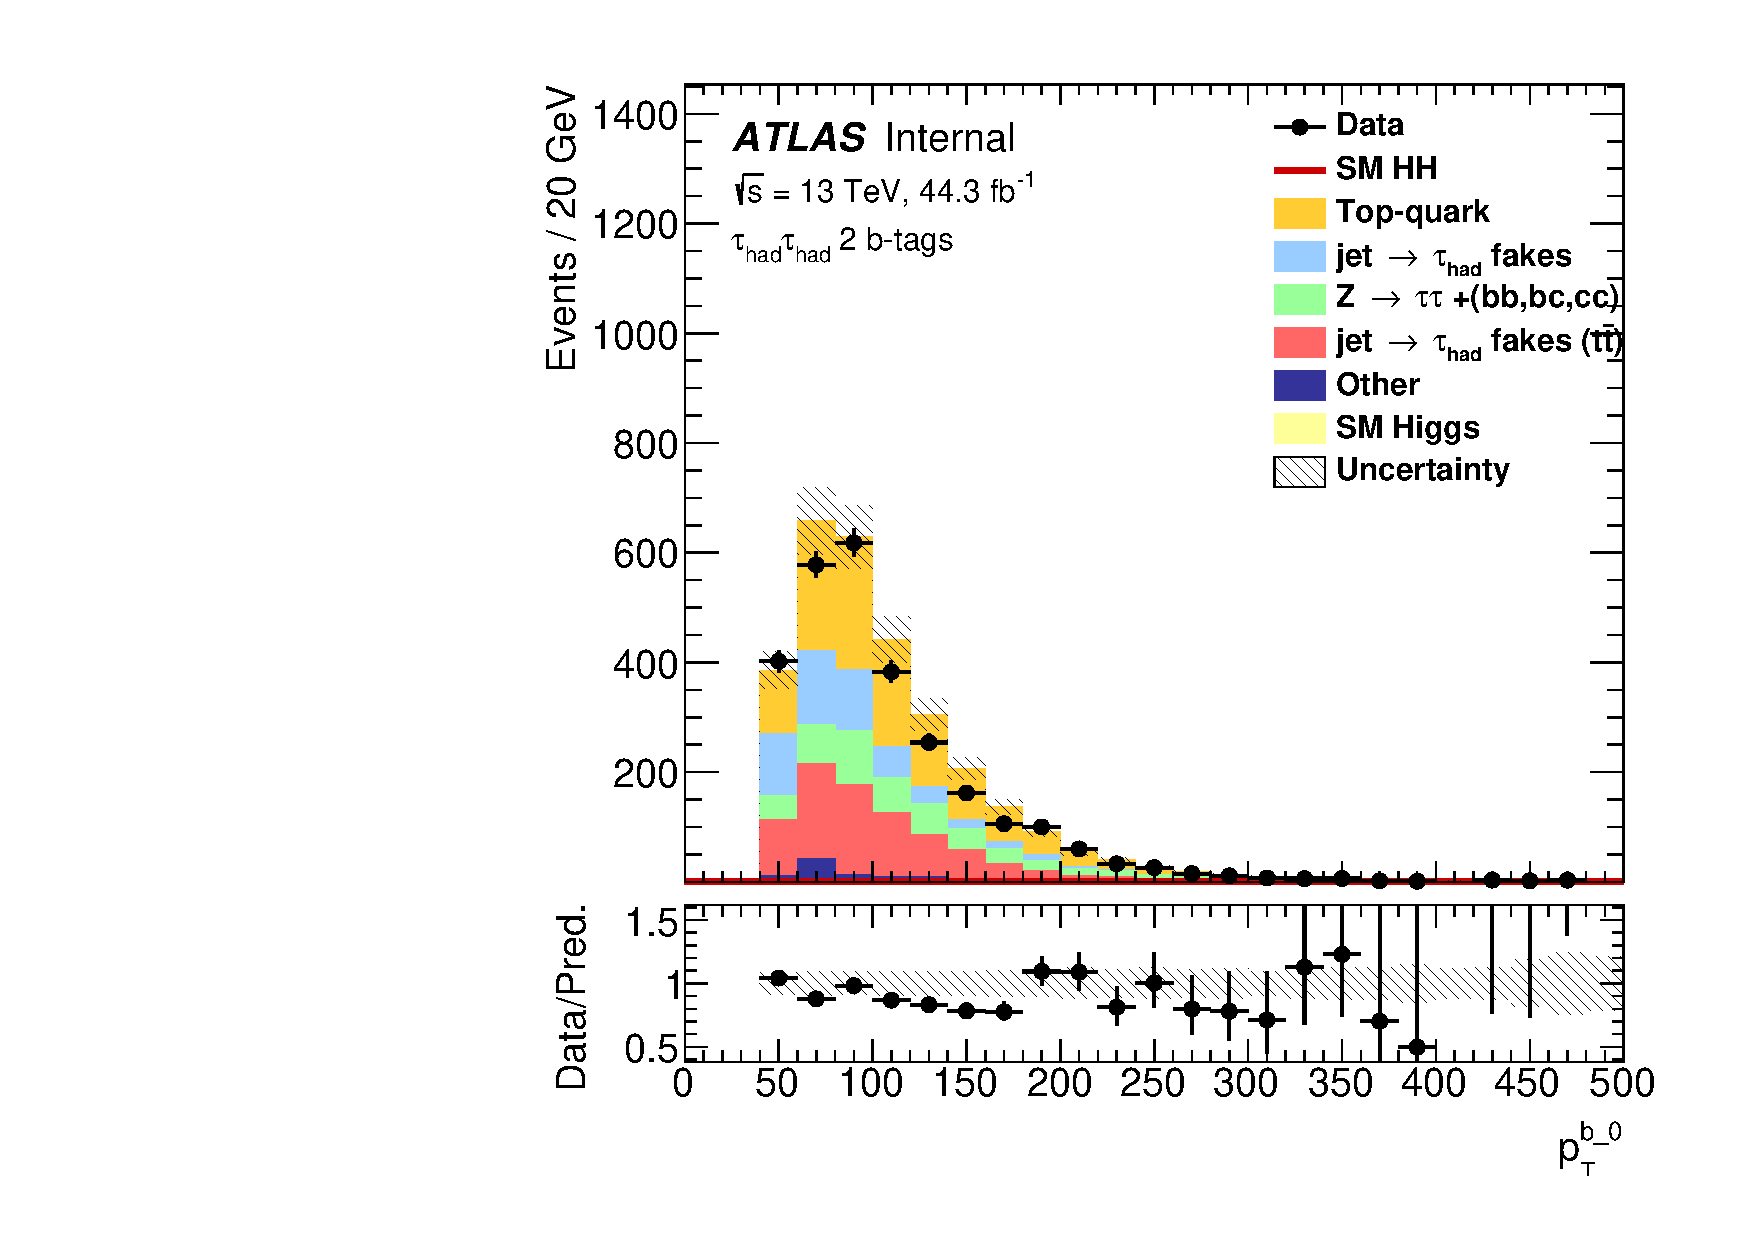
\includegraphics[width=.45\textwidth]{figures/selection/HadHad_HH/Plots2017/Region_BMin0_incJet1_distJet0Pt_J2_Y2015_DLLOS_T2_SpcTauHH_L0_Prefit.pdf}
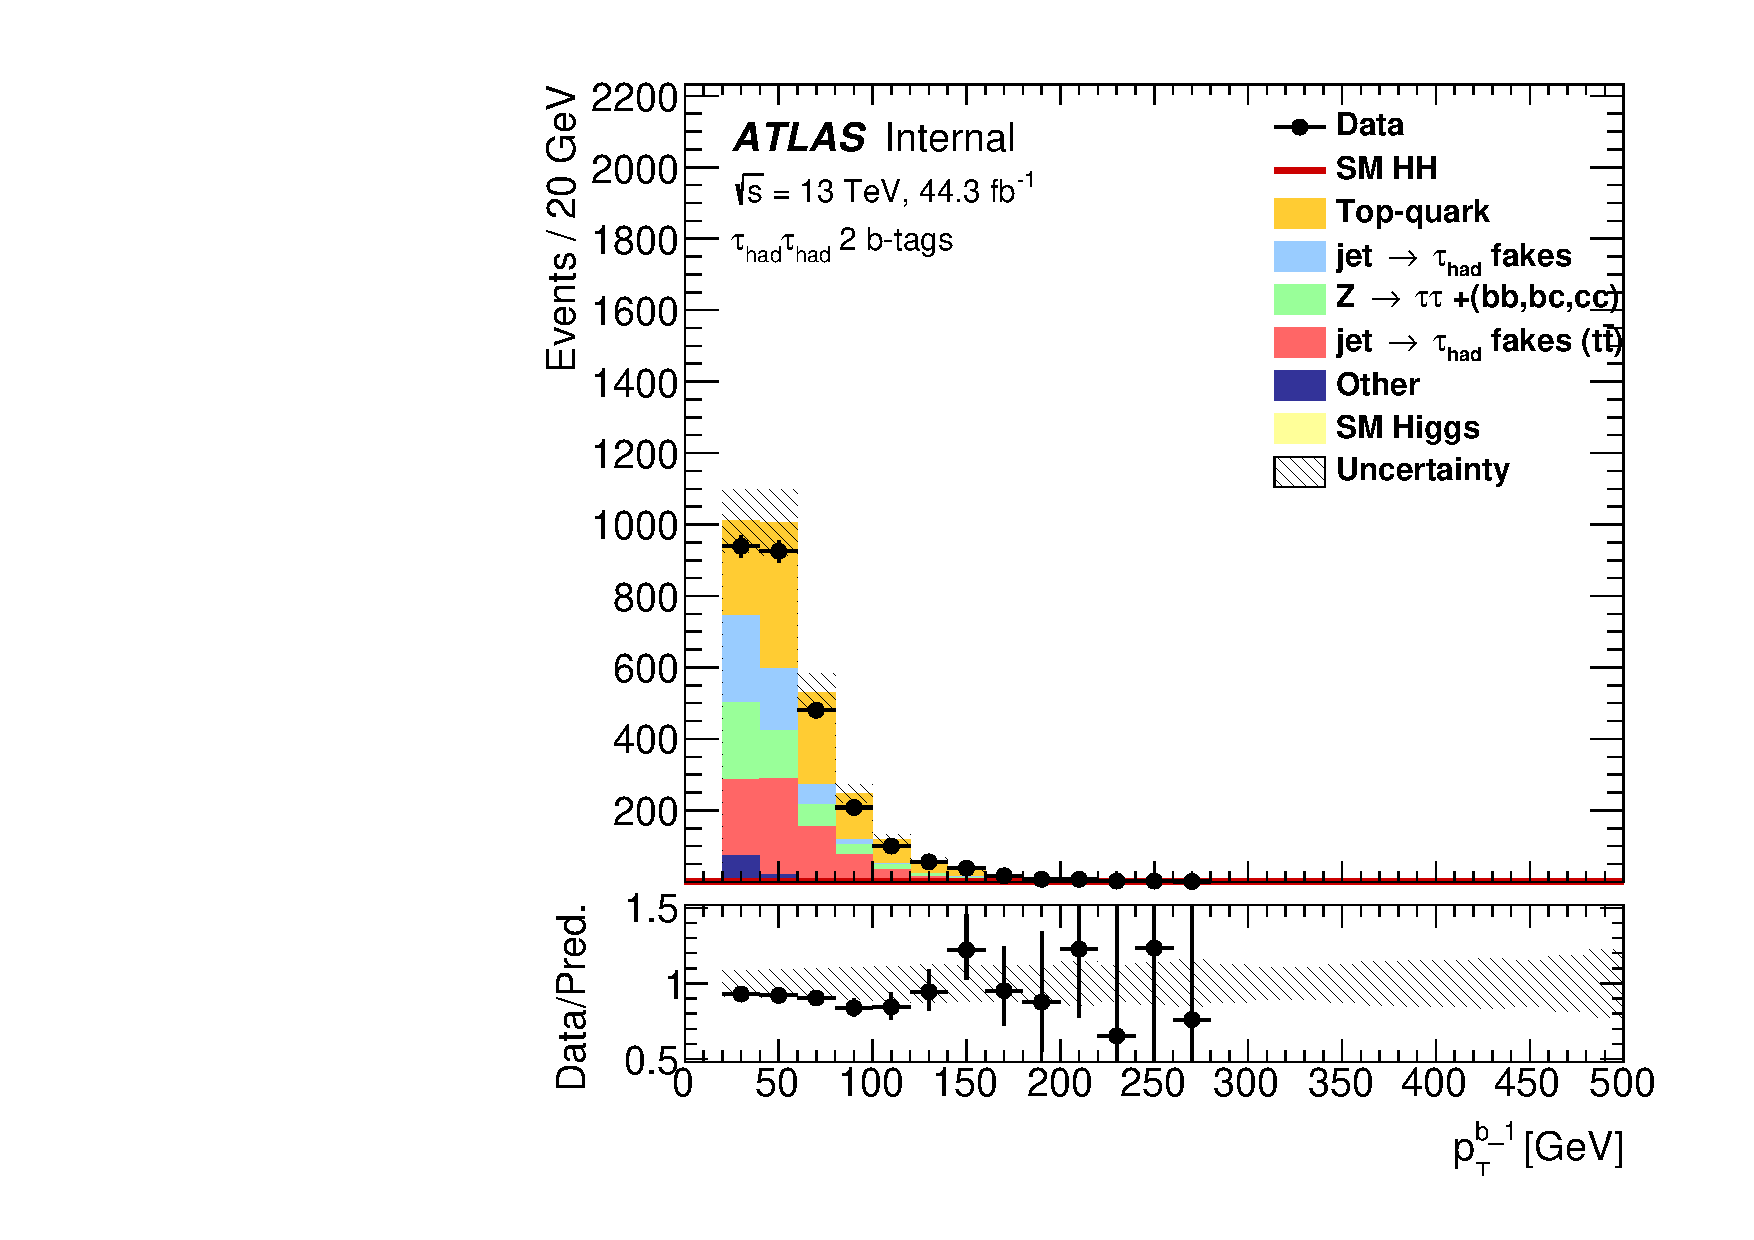
\includegraphics[width=.45\textwidth]{figures/selection/HadHad_HH/Plots2017/Region_BMin0_incJet1_distJet1Pt_J2_Y2015_DLLOS_T2_SpcTauHH_L0_Prefit.pdf}
\caption{Leading and sub-leading $\tau_{had}$ \pt and $\eta$ and $b$-jet \pt pre-fit
  distributions in the di-Higgs \hadhad signal region for the 2017 data-taking period. (Inputs from 2021\_01\_15)}
\label{fig:HadHadPreselectionPtDistributions2017}
\end{figure}

\begin{figure}
\centering
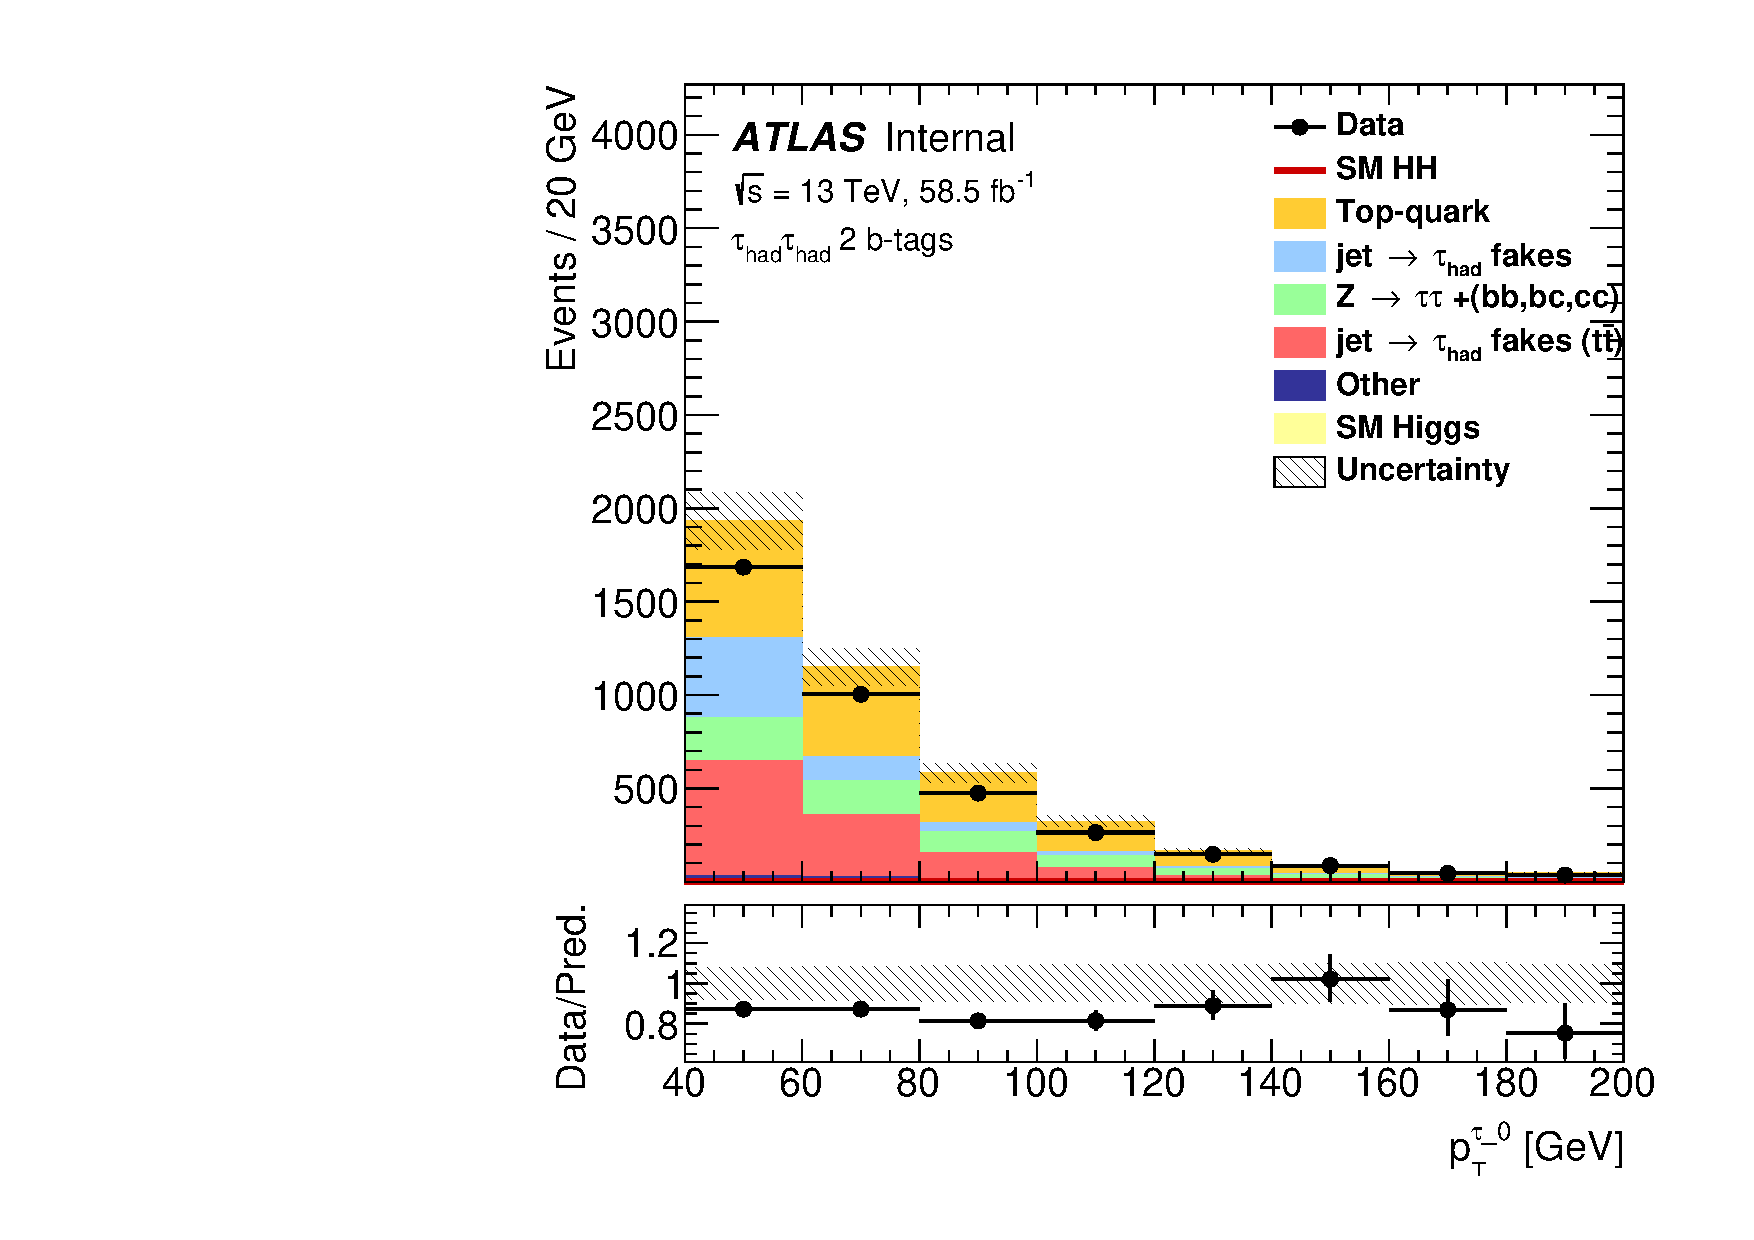
\includegraphics[width=.45\textwidth]{figures/selection/HadHad_HH/Plots2018/Region_BMin0_incJet1_distTau0Pt_J2_Y2015_DLLOS_T2_SpcTauHH_L0_Prefit.pdf}
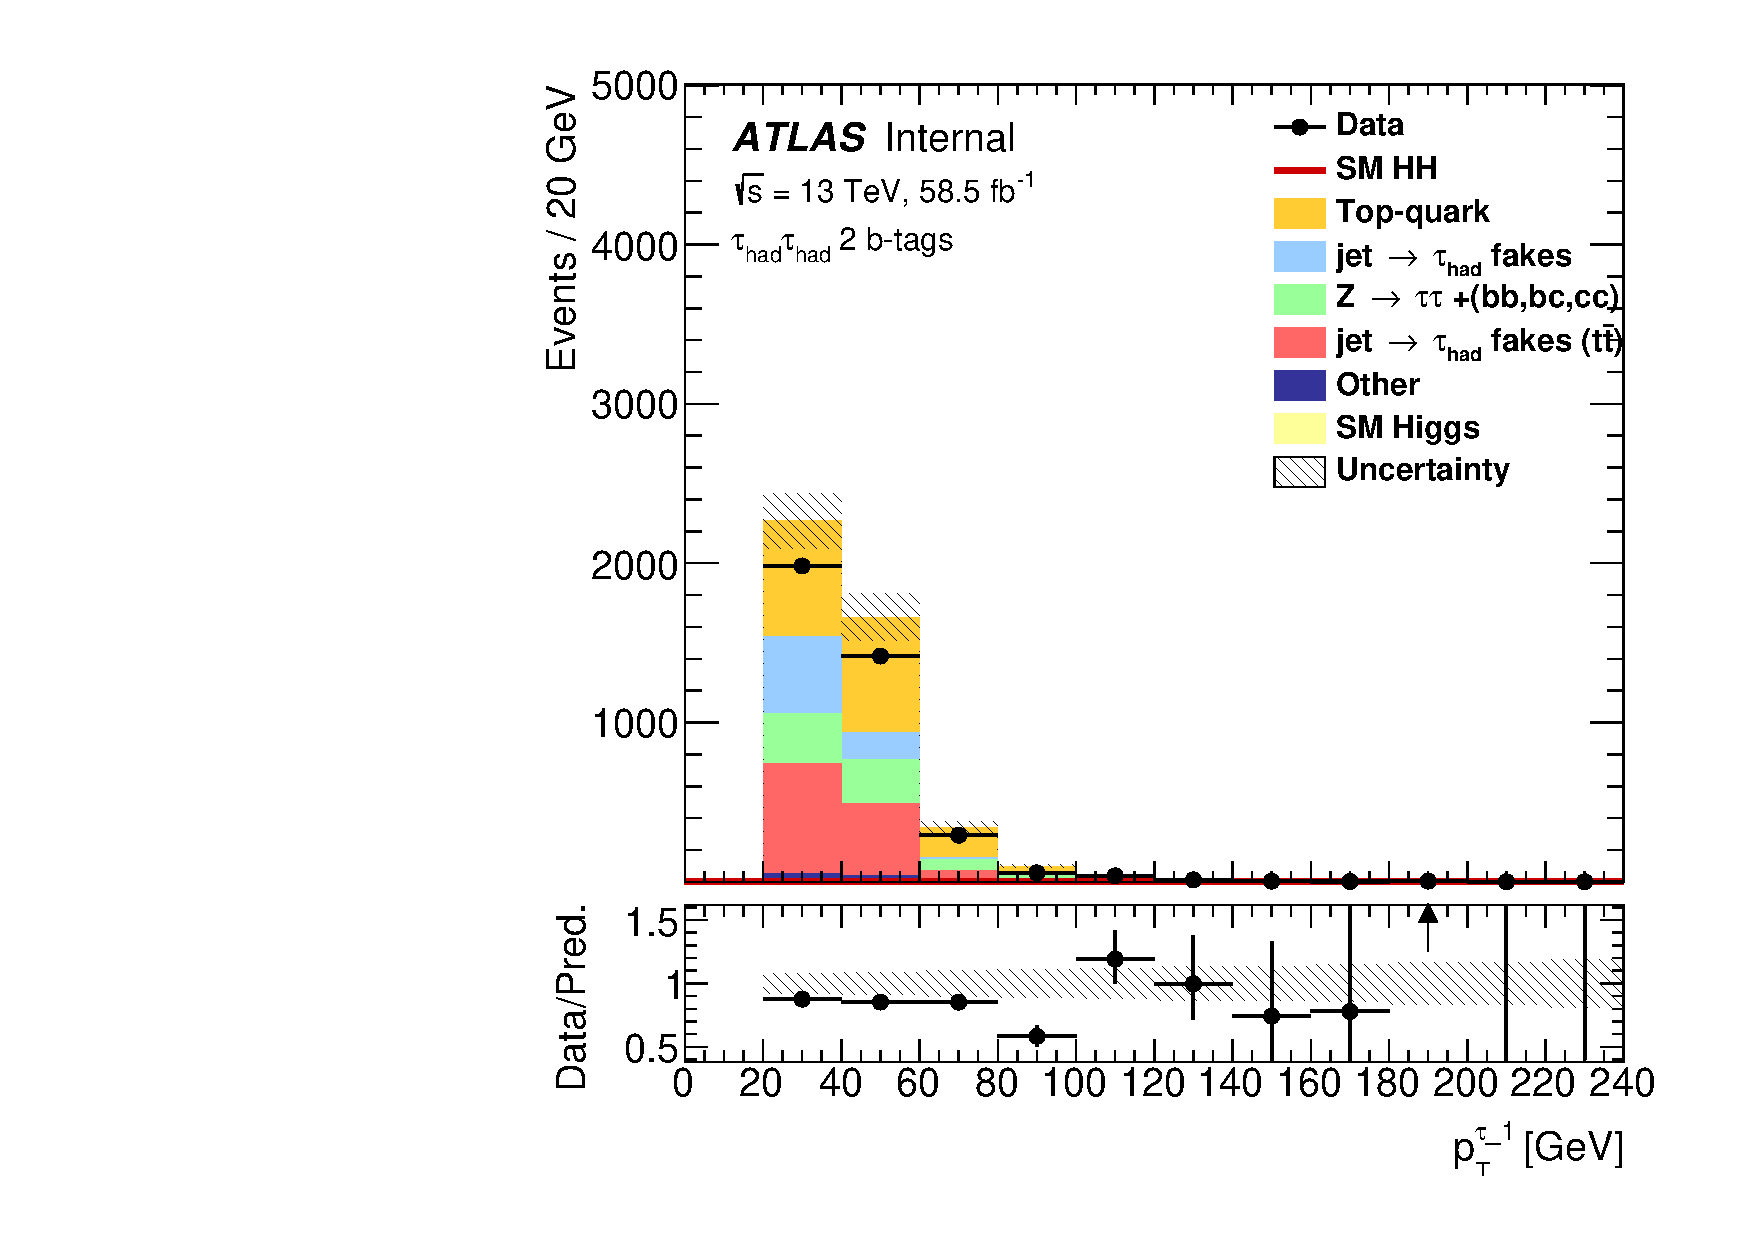
\includegraphics[width=.45\textwidth]{figures/selection/HadHad_HH/Plots2018/Region_BMin0_incJet1_distTau1Pt_J2_Y2015_DLLOS_T2_SpcTauHH_L0_Prefit.pdf}\\
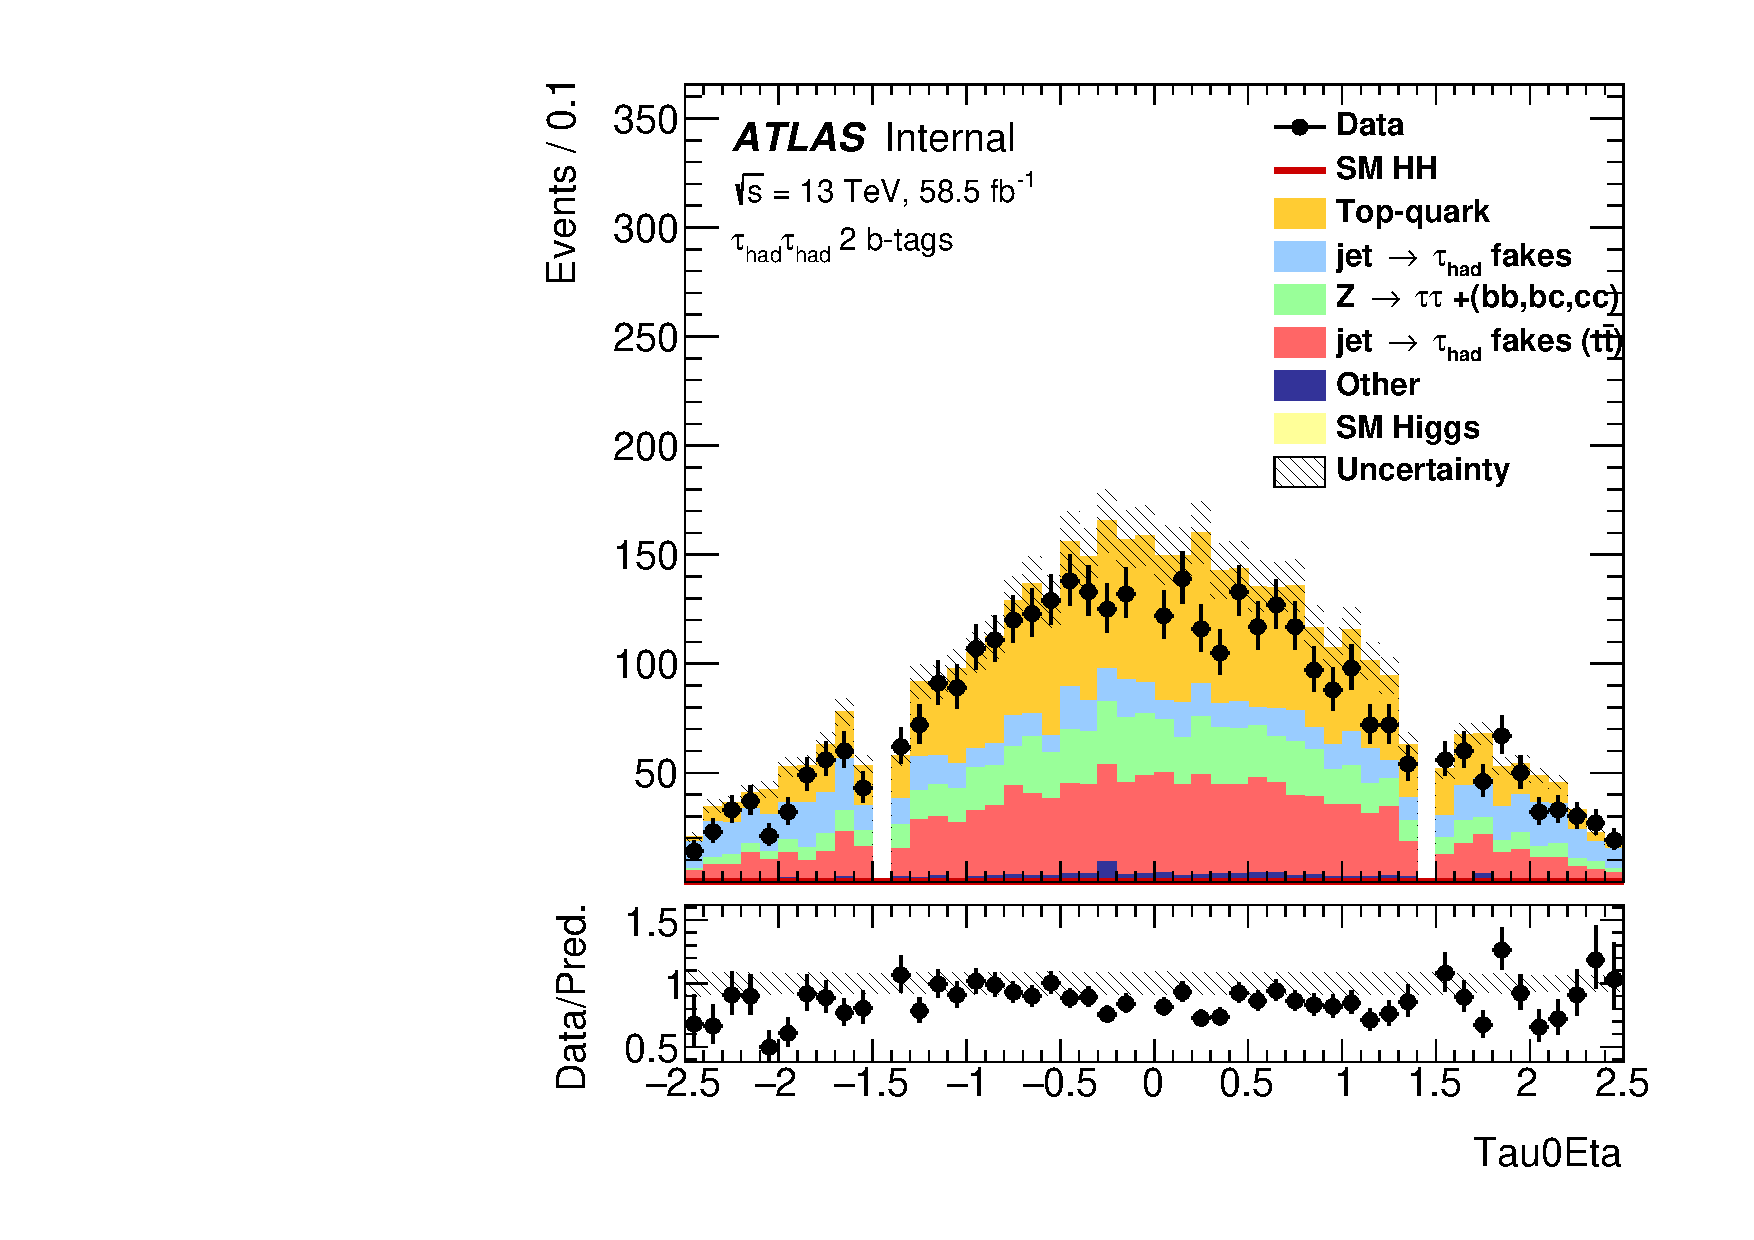
\includegraphics[width=.45\textwidth]{figures/selection/HadHad_HH/Plots2018/Region_BMin0_incJet1_distTau0Eta_J2_Y2015_DLLOS_T2_SpcTauHH_L0_Prefit.pdf}
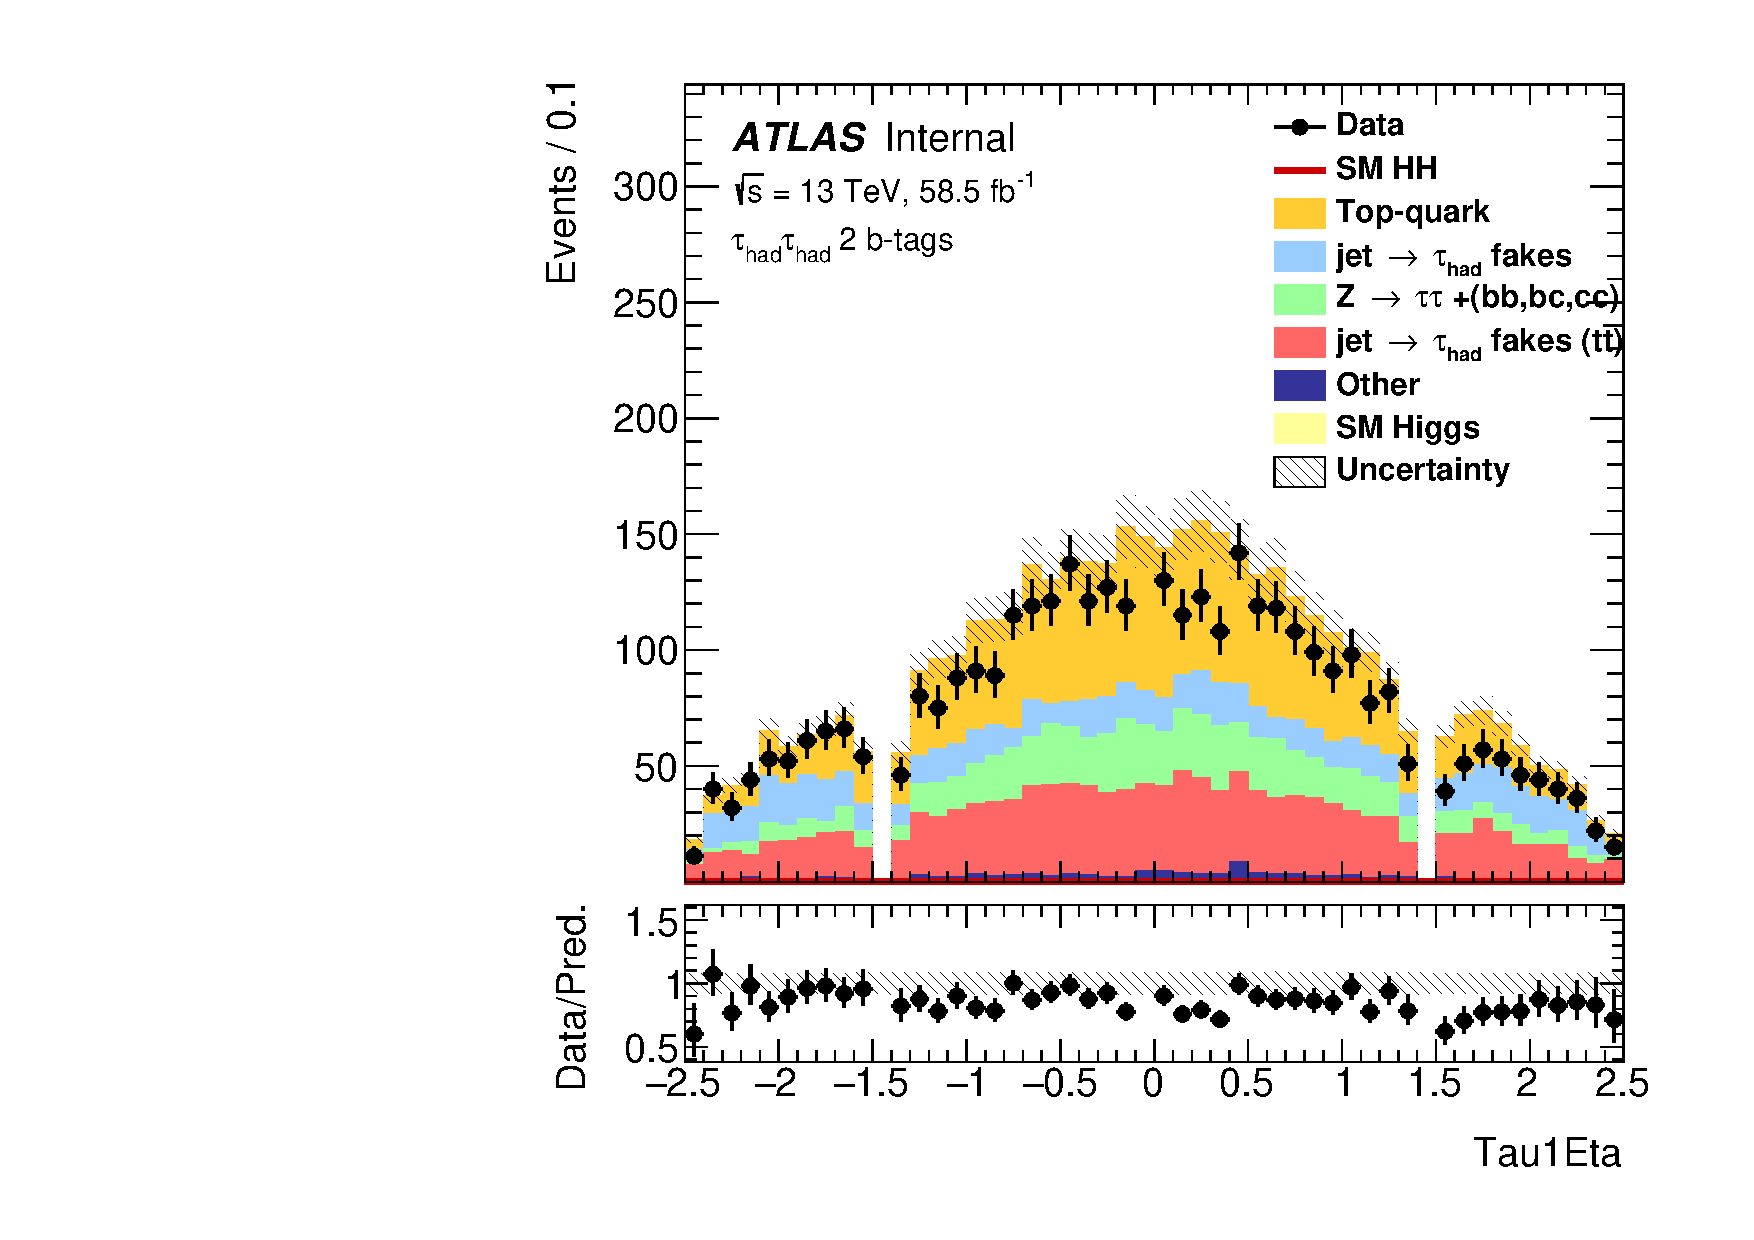
\includegraphics[width=.45\textwidth]{figures/selection/HadHad_HH/Plots2018/Region_BMin0_incJet1_distTau1Eta_J2_Y2015_DLLOS_T2_SpcTauHH_L0_Prefit.pdf}\\
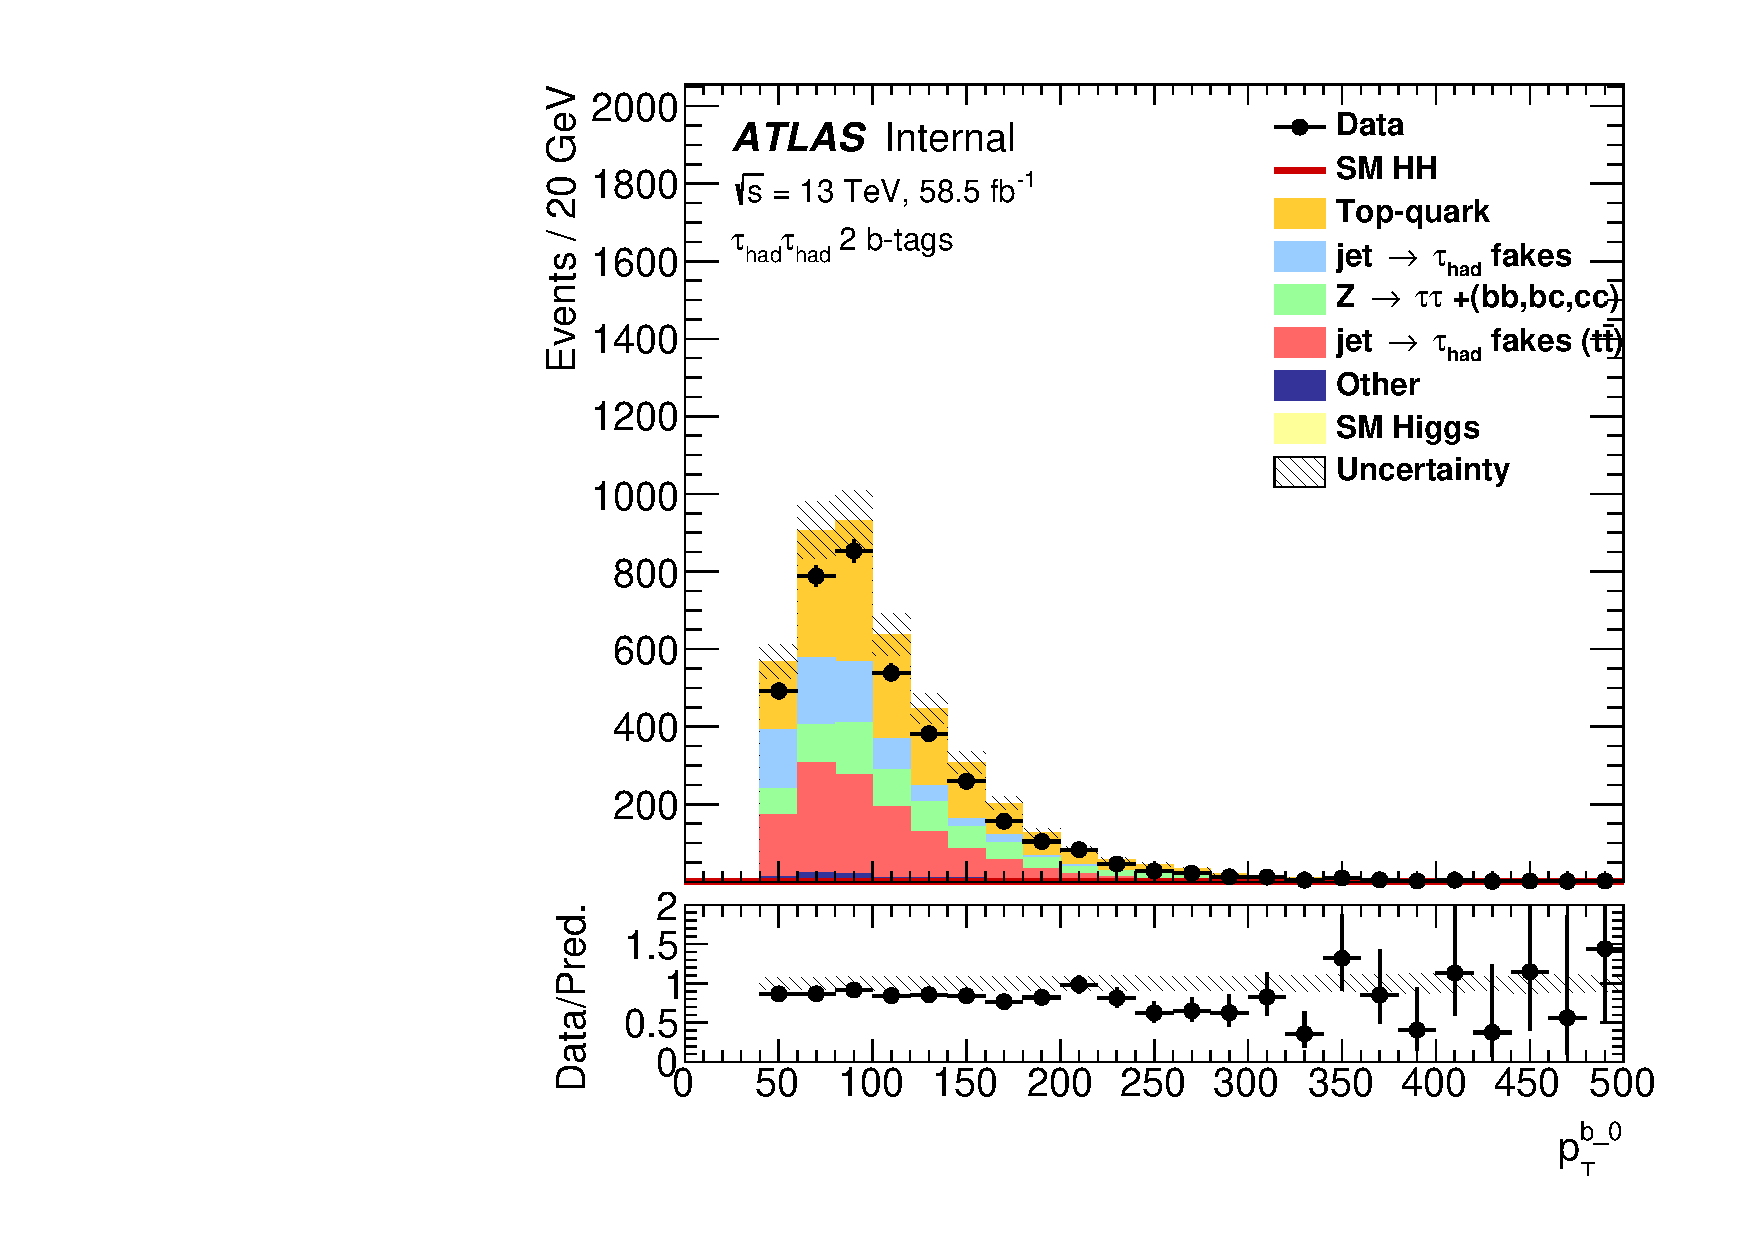
\includegraphics[width=.45\textwidth]{figures/selection/HadHad_HH/Plots2018/Region_BMin0_incJet1_distJet0Pt_J2_Y2015_DLLOS_T2_SpcTauHH_L0_Prefit.pdf}
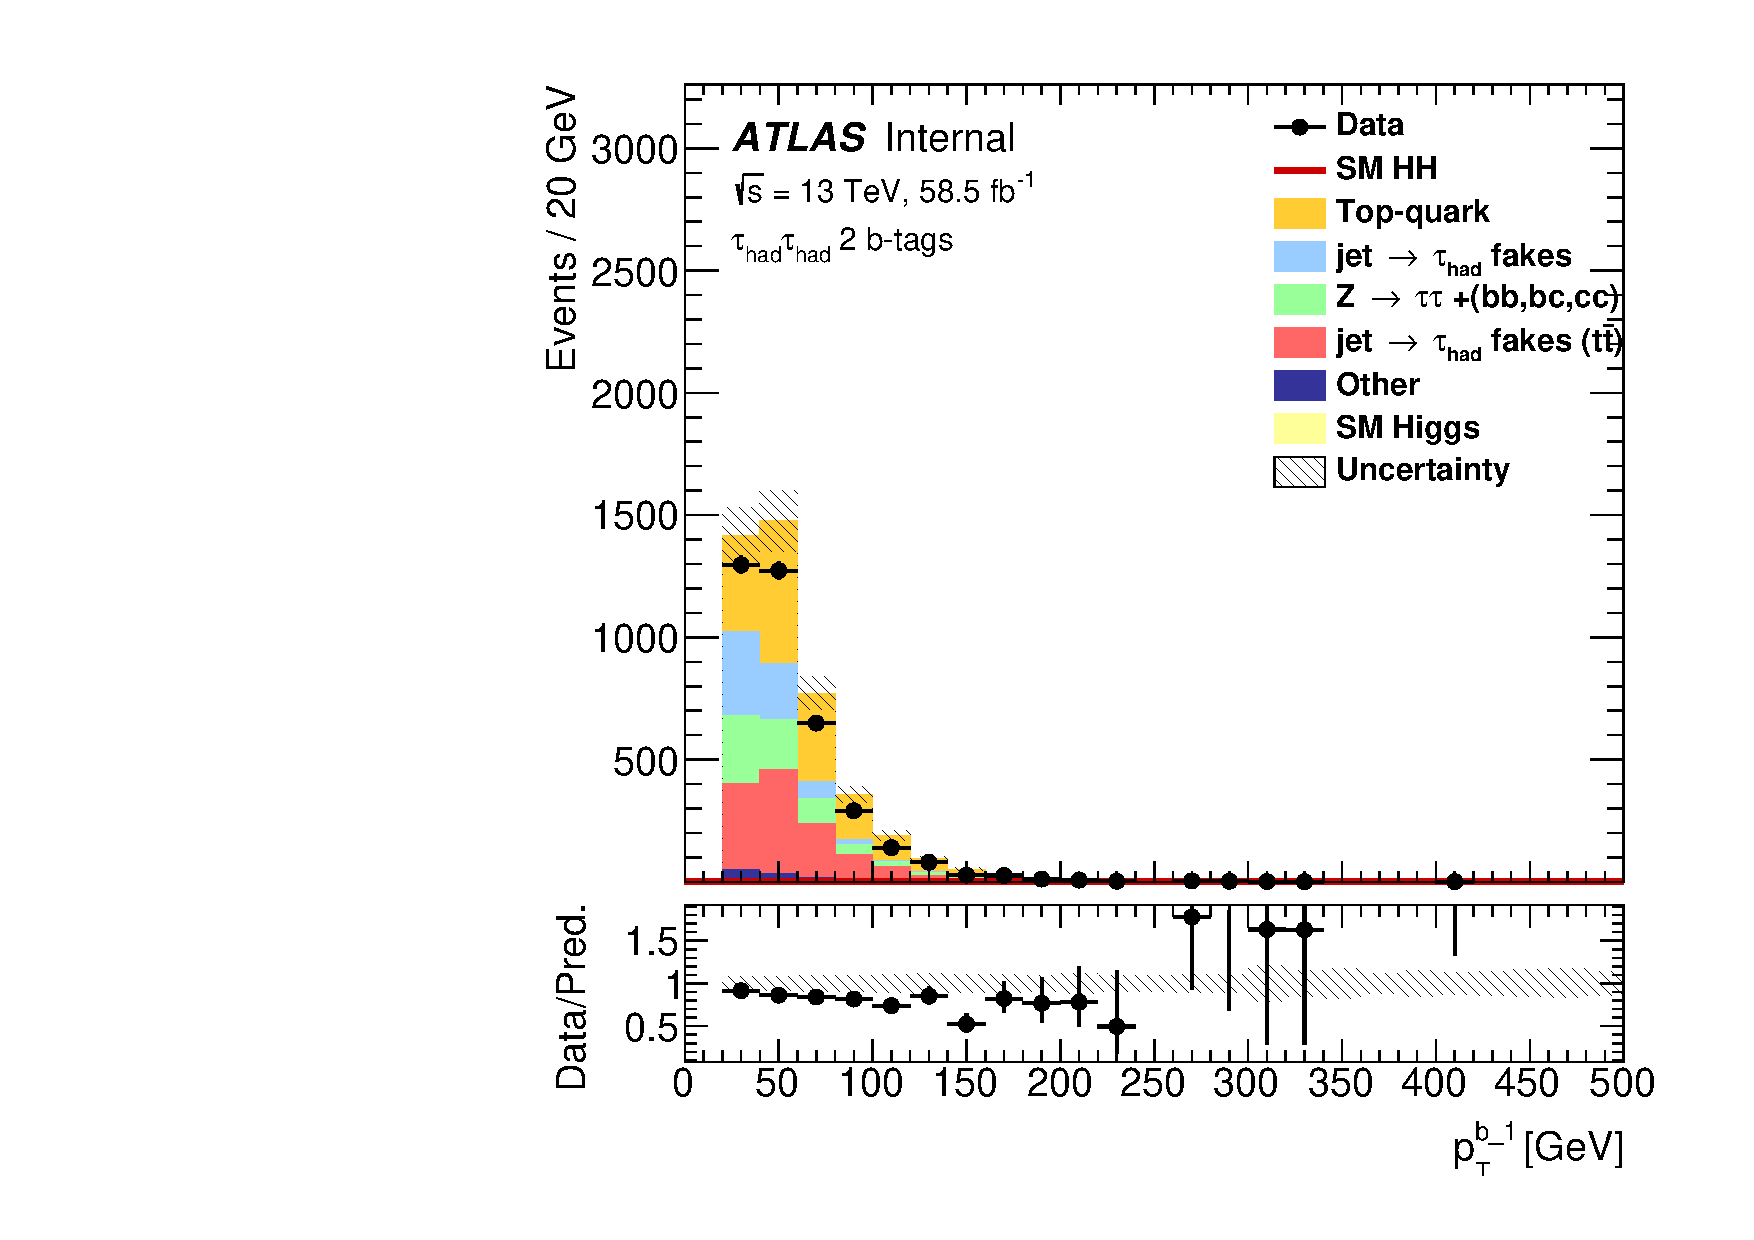
\includegraphics[width=.45\textwidth]{figures/selection/HadHad_HH/Plots2018/Region_BMin0_incJet1_distJet1Pt_J2_Y2015_DLLOS_T2_SpcTauHH_L0_Prefit.pdf}
\caption{Leading and sub-leading $\tau_{had}$ \pt and $\eta$ and $b$-jet \pt pre-fit
  distributions in the di-Higgs \hadhad signal region for the 2018 data-taking period. (Inputs from 2021\_01\_15)}
\label{fig:HadHadPreselectionPtDistributions2018}
\end{figure}

Table~\ref{tab:HadHadYields} reports the event yields after applying the $bb\hadhad$ event selection.

Figure~\ref{fig:HadHadPreselectionSignalAcceptance} shows the acceptance times efficiency of the \hadhad channel selection for the di-Higgs resonant signals as a function of the resonance mass. The acceptance times efficiency of the \hadhad channel selection for the non-resonant SM ggF di-Higgs signal is 4.08 \%. For the VBF production of the non-resonant di-Higgs signal, the acceptance times efficiency is 2.26 \%.

Comparison of the acceptance times efficiency in this channel of this new analysis to the old analysis explaining the improvements is given in Appendix~\ref{subsec:appendix_selection_sigacc_hadhad}.

\begin{figure}
\centering
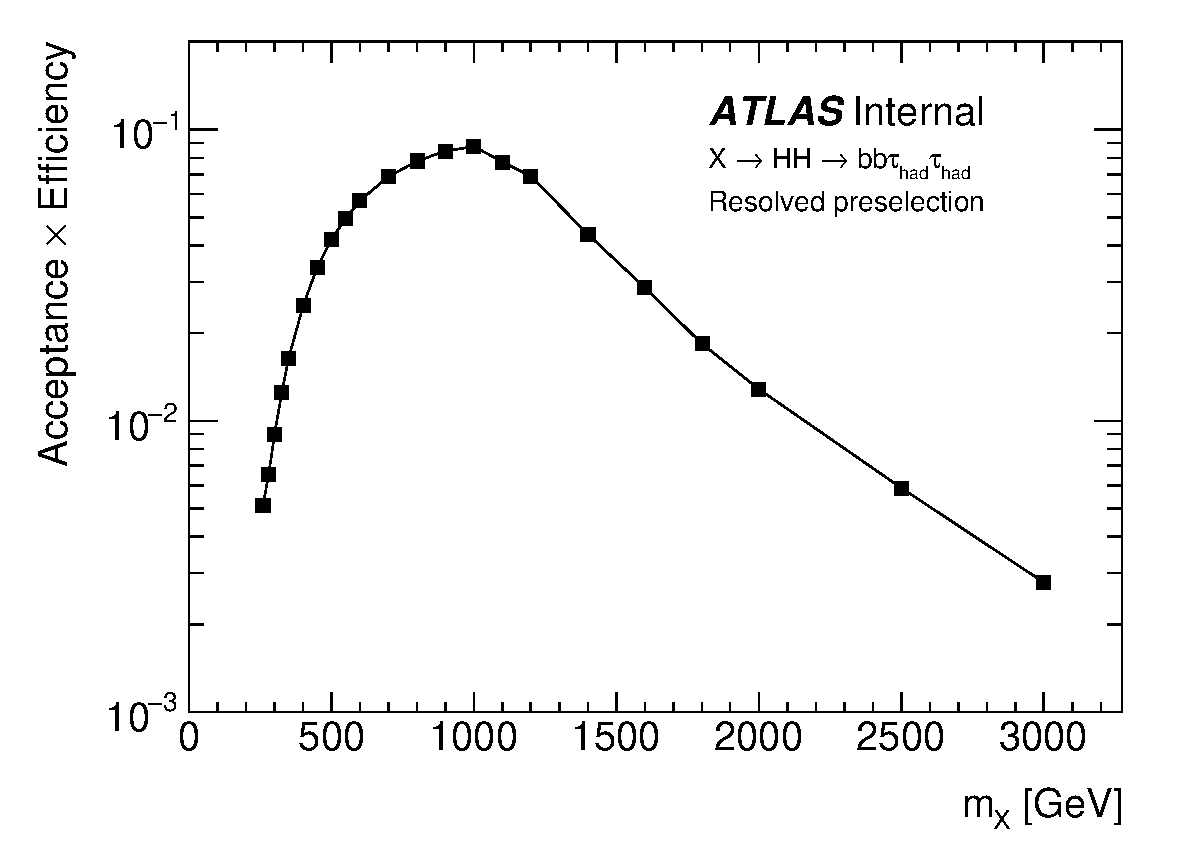
\includegraphics[width=.65\textwidth]{figures/selection/HadHad_HH/acc_times_eff}
\caption{Acceptance times efficiency of the \hadhad channel selection for the di-Higgs resonant signals as a function of the resonance mass.}
\label{fig:HadHadPreselectionSignalAcceptance}
\end{figure}


\begin{table}[]
  \centering
  \scriptsize
\begin{tabular}{|c|c|c|c|c|}
\hline
Samplename      & Entries       & Integral      & Error         & Error/Integ. \\
\hline
Hhhbbtautau1600 & 6783          & 151.606       & 1.89591       & 0.0125055 \\
Hhhbbtautau1400 & 10335         & 228.557       & 2.31767       & 0.0101405 \\
Hhhbbtautau1200 & 16458         & 356.701       & 2.86756       & 0.00803913 \\
Hhhbbtautau1100 & 34553         & 396.142       & 2.21483       & 0.00559099 \\
Hhhbbtautau1000 & 39095         & 437.269       & 2.29697       & 0.00525299 \\
Hhhbbtautau900  & 38406         & 425.43        & 2.25069       & 0.00529038 \\
Hhhbbtautau800  & 46730         & 393.532       & 1.97188       & 0.00501073 \\
Hhhbbtautau700  & 42324         & 349.682       & 1.83682       & 0.00525283 \\
Hhhbbtautau600  & 35859         & 289.018       & 1.64761       & 0.00570073 \\
Hhhbbtautau550  & 32183         & 254.681       & 1.53096       & 0.00601127 \\
Hhhbbtautau500  & 28147         & 216.619       & 1.39304       & 0.00643082 \\
Hhhbbtautau450  & 29693         & 174.027       & 1.03694       & 0.0059585 \\
Hhhbbtautau400  & 22998         & 128.518       & 0.870567      & 0.0067739 \\
Hhhbbtautau375  & 19397         & 106.977       & 0.790256      & 0.00738715 \\
Hhhbbtautau350  & 25720         & 84.6505       & 0.54268       & 0.00641083 \\
Hhhbbtautau325  & 20369         & 64.58         & 0.465808      & 0.00721288 \\
Hhhbbtautau300  & 15098         & 45.8639       & 0.383928      & 0.00837103 \\
Hhhbbtautau280  & 14485         & 33.5209       & 0.286617      & 0.00855039 \\
Hhhbbtautau260  & 11709         & 25.815        & 0.246017      & 0.00952999 \\
Hhhbbtautau251  & 12621         & 27.2638       & 0.250045      & 0.00917132 \\
hhttbbVBFSM     & 37974         & 0.166899      & 0.000882937   & 0.00529025 \\
hhttbbggFSM     & 111552        & 5.40058       & 0.0193445     & 0.00358194 \\
\hline
Fake            & 119664        & 1354.66       & 25.8309       & 0.0190681 \\
ttbarSFFF       & 1510          & 358.921       & 10.1382       & 0.0282464 \\
ttbarSFFT       & 5468          & 698.522       & 10.2809       & 0.0147181 \\
ttbarSFTF       & 9223          & 1433.95       & 16.0457       & 0.0111899 \\
ttbar           & 22937         & 3580.69       & 24.734        & 0.00690762 \\
stopWt          & 1828          & 239.007       & 5.85533       & 0.0244986 \\
stopt           & 138           & 31.4158       & 3.04587       & 0.0969535 \\
stops           & 58            & 1.66692       & 0.231854      & 0.139092 \\
Zbb             & 30            & 1.23201       & 0.253941      & 0.20612 \\
Zbc             & 4             & 0.211169      & 0.129463      & 0.613078 \\
Zbl             & 0             & 0     & 0     & 0 \\
Zcc             & 0             & 0     & 0     & 0 \\
Zcl             & 0             & 0     & 0     & 0 \\
Zl              & 1             & 0.391639      & 0.391639      & 1 \\
Zttbb           & 27512         & 1332.46       & 16.4981       & 0.0123817 \\
Zttbc           & 2375          & 140.201       & 5.80802       & 0.0414263 \\
Zttbl           & 1544          & 54.8843       & 3.0808        & 0.0561327 \\
Zttcc           & 719           & 89.8517       & 12.1893       & 0.13566 \\
Zttcl           & 431           & 30.4873       & 3.82835       & 0.125572 \\
Zttl            & 195           & 23.8278       & 36.69         & 1.5398 \\
Wtt             & 457           & 52.269        & 6.50357       & 0.124425 \\
W               & 12            & 0.864665      & 0.292456      & 0.338231 \\
VBFHtautau      & 763           & 1.64109       & 0.0622571     & 0.0379364 \\
ggFHtautau      & 1155          & 14.054        & 0.542865      & 0.0386271 \\
ZHtautau        & 1729          & 8.01903       & 0.204466      & 0.0254976 \\
WHtautau        & 48            & 0.410149      & 0.0630599     & 0.153749 \\
ZHbb            & 62251         & 14.6234       & 0.216057      & 0.0147748 \\
WHbb            & 218           & 0.164501      & 0.0175373     & 0.106609 \\
WW              & 10            & 1.91138       & 0.728729      & 0.381258 \\
WZ              & 373           & 8.8442        & 0.743756      & 0.0840954 \\
ZZ              & 2382          & 33.2378       & 1.23828       & 0.0372553 \\
ttW             & 4850          & 13.6032       & 0.299571      & 0.0220222 \\
ttZ             & 34755         & 32.3468       & 0.482682      & 0.0149221 \\
ttH             & 25696         & 34.6773       & 0.249151      & 0.00718483 \\
\hline
bkg:            & 328336        & 9589.05  &&\\
data            & 8380          & 8380 && \\
\hline
\end{tabular}
\caption{Pre-fit event yields in the di-Higgs $bb\hadhad$ signal
  region. Here, Zttjj represents the processes as $Z\rightarrow\tau\tau + jj$,
whereas Zjj represents  $Z\rightarrow ee/\mu\mu + jj$. The yields for Zttbb, Zttbc and Zttcc are scaled by 1.3. (Inputs from 2021\_06\_17)}
\label{tab:HadHadYields}
\end{table}

The cutflows for non-resonant \hadhad SM ggF and VBF signal, as well as for resonant signals at various mass points are shown in Table~\ref{tab:SMHH_hadhad_cutflow} to Table~\ref{tab:X1000_hadhad_cutflow}.
% ggF SM HH
\begin{landscape}
\begin{table}
\centering

\begin{tabular}{|c|cc|cc|cc|}
\hline
Description & \multicolumn{2}{c|}{Number of events} & \multicolumn{2}{c|}{Efficiency [\%]} & \multicolumn{2}{c|}{Relative Efficiency [\%] }\\
\hline
& STT & DTT & STT &  DTT &  STT &  DTT \\
\hline
$HH$ & \multicolumn{2}{c|}{4314.87} & \multicolumn{2}{c|}{x} & \multicolumn{2}{c|}{x} \\
$HH\rightarrow bb\tau\tau$ & \multicolumn{2}{c|}{315.23} & \multicolumn{2}{c|}{x} & \multicolumn{2}{c|}{x} \\
$HH\rightarrow bb\tau_{h}\tau_{h}$ & \multicolumn{2}{c|}{132.32} & \multicolumn{2}{c|}{100.00} & \multicolumn{2}{c|}{100.00} \\
Generator filter & \multicolumn{2}{c|}{102.78} & \multicolumn{2}{c|}{77.68} & \multicolumn{2}{c|}{77.68} \\
Derivation skimming & \multicolumn{2}{c|}{88.28} & \multicolumn{2}{c|}{66.72} & \multicolumn{2}{c|}{85.89} \\
Object preselection & \multicolumn{2}{c|}{40.44} & \multicolumn{2}{c|}{30.56} & \multicolumn{2}{c|}{45.81} \\
\hline
Trigger selection (online+offline) & \multicolumn{2}{c|}{17.30} & \multicolumn{2}{c|}{13.08} & \multicolumn{2}{c|}{42.79} \\
Trigger category & 1.95 & 15.35 & 1.48 & 11.60 & 11.29 & 88.71 \\
\hline
Random $\tau$ selection & 1.93 & 15.31 & 1.46 & 11.57 & 99.03 & 99.78 \\
Object selection ($n_\tau=2$, further requirements on jets and tau-jet OLR) & 1.86 & 14.12 & 1.40 & 10.67 & 95.92 & 92.19 \\
Pileup Correction & 1.91 & 14.40 & 1.44 & 10.88 & x & x \\
2 Loose $\tau$s (one Loose $\tau$ already required in derivation) & 1.37 & 11.64 & 1.04 & 8.80 & 71.95 & 80.84 \\
Subleading $\tau$ \pt>25 GeV& 1.21 & 11.64 & 0.91 & 8.80 & 87.74 & x \\
\hline
MMC > 60 GeV& 1.15 & 11.40 & 0.87 & 8.62 & 95.40 & 97.98 \\
At least one jet with $\pT > 45$ GeV & 1.15 & 11.17 & 0.87 & 8.44 & 99.63 & 97.95 \\
DTT offline jet cuts & 1.15 & 9.95 & 0.87 & 7.52 & x & 89.05 \\
Scale Factors & 1.16 & 10.48 & 0.87 & 7.92 & x &x \\
Opposite charge sign & 1.14 & 10.34 & 0.86 & 7.82 & 98.14 & 98.71 \\
Both jets are b-tagged & 0.57 & 4.83 & 0.43 & 3.65 & 49.86 & 46.74 \\
\hline
\end{tabular}
\caption{Non-resonant \hadhad SM ggF signal cutflow (Powheg+Pythia8).}
\label{tab:SMHH_hadhad_cutflow}
\end{table}
\end{landscape}


% VBF SM HH
\begin{landscape}
\begin{table}
\centering

\begin{tabular}{|c|cc|cc|cc|}
\hline
Description & \multicolumn{2}{c|}{Number of events} & \multicolumn{2}{c|}{Efficiency [\%]} & \multicolumn{2}{c|}{Relative Efficiency [\%] }\\
\hline
& STT & DTT & STT &  DTT &  STT &  DTT \\
\hline
$HH$ & \multicolumn{2}{c|}{239.85} & \multicolumn{2}{c|}{x} & \multicolumn{2}{c|}{x} \\
$HH\rightarrow bb\tau\tau$ & \multicolumn{2}{c|}{17.52} & \multicolumn{2}{c|}{x} & \multicolumn{2}{c|}{x} \\
$HH\rightarrow bb\tau_{h}\tau_{h}$ & \multicolumn{2}{c|}{7.36} & \multicolumn{2}{c|}{100.00} & \multicolumn{2}{c|}{100.00} \\
Generator filter & \multicolumn{2}{c|}{5.00} & \multicolumn{2}{c|}{67.99} & \multicolumn{2}{c|}{67.99} \\
Derivation skimming & \multicolumn{2}{c|}{4.24} & \multicolumn{2}{c|}{57.61} & \multicolumn{2}{c|}{84.73} \\
Object preselection & \multicolumn{2}{c|}{1.89} & \multicolumn{2}{c|}{25.69} & \multicolumn{2}{c|}{44.59} \\
\hline
Trigger selection (online+offline) & \multicolumn{2}{c|}{0.74} & \multicolumn{2}{c|}{10.11} & \multicolumn{2}{c|}{39.36} \\
Trigger category & 0.06 & 0.69 & 0.79 & 9.32 & 7.82  & 92.18 \\
\hline
Random $\tau$ selection & 0.06 & 0.68 & 0.78 & 9.28 & 98.64 & 99.55 \\
Object selection ($n_\tau=2$, further requirements on jets and tau-jet OLR) & 0.05 & 0.59 & 0.72 & 7.99 & 92.33 & 86.07 \\
Pileup Correction & 0.05 & 0.60 & 0.74 & 8.13 & x	  & x\\
2 Loose $\tau$s (one Loose $\tau$ already required in derivation) & 0.04 & 0.48 & 0.56 & 6.54 & 74.81 & 80.37 \\
Subleading $\tau$ \pt>25 GeV& 0.04 & 0.48 & 0.49 & 6.54 & 88.41 & x\\
\hline
MMC > 60 GeV& 0.03 & 0.47 & 0.47 & 6.37 & 95.60 & 97.52 \\
At least one jet with $\pT > 45$ GeV & 0.03 & 0.45 & 0.46 & 6.07 & 98.65 & 95.26 \\
DTT offline jet cuts & 0.03 & 0.35 & 0.46 & 4.80 & x	  & 78.99 \\
Scale Factors & 0.03 & 0.37 & 0.47 & 5.03 & x	  & x\\
Opposite charge sign & 0.03 & 0.36 & 0.46 & 4.94 & 97.86 & 98.19 \\
Both jets are b-tagged & 0.01 & 0.15 & 0.20 & 2.07 & 42.67 & 41.98 \\
\hline
\end{tabular}
\caption{Non-resonant \hadhad SM VBF signal cutflow.}
\label{tab:SMVBFHH_hadhad_cutflow}
\end{table}
\end{landscape}


% X300
\begin{landscape}
\begin{table}
\centering

\begin{tabular}{|c|cc|cc|cc|}
\hline
Description & \multicolumn{2}{c|}{Number of events} & \multicolumn{2}{c|}{Efficiency [\%]} & \multicolumn{2}{c|}{Relative Efficiency [\%] }\\
\hline
& STT & DTT & STT &  DTT &  STT &  DTT \\
\hline
$HH$ & \multicolumn{2}{c|}{138965.16} & \multicolumn{2}{c|}{x} & \multicolumn{2}{c|}{x} \\
$HH\rightarrow bb\tau\tau$ & \multicolumn{2}{c|}{10152.27} & \multicolumn{2}{c|}{x} & \multicolumn{2}{c|}{x} \\
$HH\rightarrow bb\tau_{h}\tau_{h}$ & \multicolumn{2}{c|}{4261.66} & \multicolumn{2}{c|}{100.00} & \multicolumn{2}{c|}{100.00} \\
Generator filter & \multicolumn{2}{c|}{2652.79} & \multicolumn{2}{c|}{62.25} & \multicolumn{2}{c|}{62.25} \\
Derivation skimming & \multicolumn{2}{c|}{2168.46} & \multicolumn{2}{c|}{50.88} & \multicolumn{2}{c|}{81.74} \\
Object preselection & \multicolumn{2}{c|}{924.99} & \multicolumn{2}{c|}{21.70} & \multicolumn{2}{c|}{42.66} \\
\hline
Trigger selection (online+offline) & \multicolumn{2}{c|}{278.89} & \multicolumn{2}{c|}{6.54} & \multicolumn{2}{c|}{30.15} \\
Trigger category & 0.63 & 278.26 & 0.01 & 6.53 & 0.23   & 99.77  \\
\hline
Random $\tau$ selection & 0.63 & 277.68 & 0.01 & 6.52 & 99.55  & 99.79  \\
Object selection ($n_\tau=2$, further requirements on jets and tau-jet OLR) & 0.58 & 251.00 & 0.01 & 5.89 & 92.79  & 90.39  \\
Pileup Correction & 0.65 & 256.04 & 0.02 & 6.01 & x      & x \\
2 Loose $\tau$s (one Loose $\tau$ already required in derivation) & 0.43 & 200.67 & 0.01 & 4.71 & 66.48  & 78.38  \\
Subleading $\tau$ \pt>25 GeV& 0.32 & 200.67 & 0.01 & 4.71 & 74.60  & x \\
\hline
MMC > 60 GeV& 0.32 & 198.33 & 0.01 & 4.65 & 98.85  & 98.83  \\
At least one jet with $\pT > 45$ GeV & 0.29 & 179.85 & 0.01 & 4.22 & 90.34  & 90.68  \\
DTT offline jet cuts & 0.29 & 104.73 & 0.01 & 2.46 & x      & 58.23  \\
Scale Factors & 0.28 & 106.45 & 0.01 & 2.50 & x      & x \\
Opposite charge sign & 0.28 & 105.04 & 0.01 & 2.46 & 100.00 & 98.68  \\
Both jets are b-tagged & 0.13 & 45.73  & 0.00 & 1.07 & 47.49  & 43.54  \\
\hline
\end{tabular}
\caption{300~GeV resonant \hadhad signal cutflow. Assuming $\sigma(pp\rightarrow X\rightarrow HH)=1$~pb}
\label{tab:X300_hadhad_cutflow}
\end{table}
\end{landscape}


% X500
\begin{landscape}
\begin{table}
\centering

\begin{tabular}{|c|cc|cc|cc|}
\hline
Description & \multicolumn{2}{c|}{Number of events} & \multicolumn{2}{c|}{Efficiency [\%]} & \multicolumn{2}{c|}{Relative Efficiency [\%] }\\
\hline
& STT & DTT & STT &  DTT &  STT &  DTT \\
\hline
$HH$ & \multicolumn{2}{c|}{138965.16} & \multicolumn{2}{c|}{x} & \multicolumn{2}{c|}{x} \\
$HH\rightarrow bb\tau\tau$ & \multicolumn{2}{c|}{10152.27} & \multicolumn{2}{c|}{x} & \multicolumn{2}{c|}{x} \\
$HH\rightarrow bb\tau_{h}\tau_{h}$ & \multicolumn{2}{c|}{4261.66} & \multicolumn{2}{c|}{100.00} & \multicolumn{2}{c|}{100.00} \\
Generator filter & \multicolumn{2}{c|}{3256.65} & \multicolumn{2}{c|}{76.42} & \multicolumn{2}{c|}{76.42} \\
Derivation skimming & \multicolumn{2}{c|}{2843.20} & \multicolumn{2}{c|}{66.72} & \multicolumn{2}{c|}{87.30} \\
Object preselection & \multicolumn{2}{c|}{1364.93} & \multicolumn{2}{c|}{32.03} & \multicolumn{2}{c|}{48.01} \\
\hline
Trigger selection (online+offline) & \multicolumn{2}{c|}{645.23} & \multicolumn{2}{c|}{15.14} & \multicolumn{2}{c|}{47.27} \\
Trigger category & 56.96 & 588.27 & 1.34 & 13.80 & 8.83  & 91.17  \\
\hline
Random $\tau$ selection & 56.56 & 587.17 & 1.33 & 13.78 & 99.29 & 99.81  \\
Object selection ($n_\tau=2$, further requirements on jets and tau-jet OLR) & 54.37 & 551.63 & 1.28 & 12.94 & 96.13 & 93.95  \\
Pileup Correction & 53.43 & 576.13 & 1.25 & 13.52 & x     & x \\
2 Loose $\tau$s (one Loose $\tau$ already required in derivation) & 38.26 & 474.59 & 0.90 & 11.14 & 71.60 & 82.38  \\
Subleading $\tau$ \pt>25 GeV& 31.28 & 474.59 & 0.73 & 11.14 & 81.76 & x \\
\hline
MMC > 60 GeV& 30.09 & 465.55 & 0.71 & 10.92 & 96.20 & 98.09  \\
At least one jet with $\pT > 45$ GeV & 29.85 & 460.32 & 0.70 & 10.80 & 99.18 & 98.88  \\
DTT offline jet cuts & 29.85 & 434.24 & 0.70 & 10.19 & x     & 94.33  \\
Scale Factors & 29.65 & 452.56 & 0.70 & 10.62 & x     & x \\
Opposite charge sign & 28.98 & 446.93 & 0.68 & 10.49 & 97.71 & 98.76  \\
Both jets are b-tagged & 13.37 & 203.25 & 0.31 & 4.77  & 46.13 & 45.48  \\
\hline
\end{tabular}
\caption{500~GeV resonant \hadhad signal cutflow. Assuming $\sigma(pp\rightarrow X\rightarrow HH)=1$~pb}
\label{tab:X500_hadhad_cutflow}
\end{table}
\end{landscape}


% X1000
\begin{landscape}
\begin{table}
\centering

\begin{tabular}{|c|cc|cc|cc|}
\hline
Description & \multicolumn{2}{c|}{Number of events} & \multicolumn{2}{c|}{Efficiency [\%]} & \multicolumn{2}{c|}{Relative Efficiency [\%] }\\
\hline
& STT & DTT & STT &  DTT &  STT &  DTT \\
\hline
$HH$ & \multicolumn{2}{c|}{138965.16} & \multicolumn{2}{c|}{x} & \multicolumn{2}{c|}{x} \\
$HH\rightarrow bb\tau\tau$ & \multicolumn{2}{c|}{10152.27} & \multicolumn{2}{c|}{x} & \multicolumn{2}{c|}{x} \\
$HH\rightarrow bb\tau_{h}\tau_{h}$ & \multicolumn{2}{c|}{4261.66} & \multicolumn{2}{c|}{100.00} & \multicolumn{2}{c|}{100.00} \\
Generator filter & \multicolumn{2}{c|}{3750.86} & \multicolumn{2}{c|}{88.01} & \multicolumn{2}{c|}{88.01} \\
Derivation skimming & \multicolumn{2}{c|}{3330.25} & \multicolumn{2}{c|}{78.14} & \multicolumn{2}{c|}{88.79} \\
Object preselection & \multicolumn{2}{c|}{1753.58} & \multicolumn{2}{c|}{41.15} & \multicolumn{2}{c|}{52.661} \\
\hline
Trigger selection (online+offline) & \multicolumn{2}{c|}{1232.55} & \multicolumn{2}{c|}{28.92} & \multicolumn{2}{c|}{70.29} \\
Trigger category & 779.77 & 452.78 & 18.30 & 10.62 & 63.26 & 36.74 \\
\hline
Random $\tau$ selection & 774.73 & 451.99 & 18.18 & 10.61 & 99.35 & 99.83 \\
Object selection ($n_\tau=2$, further requirements on jets and tau-jet OLR) & 761.35 & 437.79 & 17.87 & 10.27 & 98.27 & 96.86 \\
Pileup Correction & 774.49 & 450.27 & 18.17 & 10.57 & x     & x\\
2 Loose $\tau$s (one Loose $\tau$ already required in derivation) & 587.02 & 384.98 & 13.77 & 9.03  & 75.80 & 85.50 \\
Subleading $\tau$ \pt>25 GeV& 555.91 & 384.98 & 13.04 & 9.03  & 94.70 & x\\
\hline
MMC > 60 GeV& 530.45 & 371.21 & 12.45 & 8.71  & 95.42 & 96.42 \\
At least one jet with $\pT > 45$ GeV & 530.07 & 369.78 & 12.44 & 8.68  & 99.93 & 99.62 \\
DTT offline jet cuts & 530.07 & 353.30 & 12.44 & 8.29  & x     & 95.54 \\
Scale Factors & 531.29 & 373.62 & 12.47 & 8.77  & x     & x\\
Opposite charge sign & 520.97 & 367.95 & 12.22 & 8.63  & 98.06 & 98.48 \\
Both jets are b-tagged & 263.95 & 173.31 & 6.19  & 4.07  & 50.67 & 47.10 \\
\hline
\end{tabular}
\caption{1000~GeV resonant \hadhad signal cutflow. Assuming $\sigma(pp\rightarrow X\rightarrow HH)=1$~pb}
\label{tab:X1000_hadhad_cutflow}
\end{table}
\end{landscape}




\FloatBarrier
